% Options for packages loaded elsewhere
\PassOptionsToPackage{unicode}{hyperref}
\PassOptionsToPackage{hyphens}{url}
\PassOptionsToPackage{dvipsnames,svgnames,x11names}{xcolor}
%
\documentclass[
  12pt,
  a4paper, twoside]{book}
\usepackage{amsmath,amssymb}
\usepackage{iftex}
\ifPDFTeX
  \usepackage[T1]{fontenc}
  \usepackage[utf8]{inputenc}
  \usepackage{textcomp} % provide euro and other symbols
\else % if luatex or xetex
  \usepackage{unicode-math} % this also loads fontspec
  \defaultfontfeatures{Scale=MatchLowercase}
  \defaultfontfeatures[\rmfamily]{Ligatures=TeX,Scale=1}
\fi
\usepackage{lmodern}
\ifPDFTeX\else
  % xetex/luatex font selection
\fi
% Use upquote if available, for straight quotes in verbatim environments
\IfFileExists{upquote.sty}{\usepackage{upquote}}{}
\IfFileExists{microtype.sty}{% use microtype if available
  \usepackage[]{microtype}
  \UseMicrotypeSet[protrusion]{basicmath} % disable protrusion for tt fonts
}{}
\makeatletter
\@ifundefined{KOMAClassName}{% if non-KOMA class
  \IfFileExists{parskip.sty}{%
    \usepackage{parskip}
  }{% else
    \setlength{\parindent}{0pt}
    \setlength{\parskip}{6pt plus 2pt minus 1pt}}
}{% if KOMA class
  \KOMAoptions{parskip=half}}
\makeatother
\usepackage{xcolor}
\usepackage{longtable,booktabs,array}
\usepackage{calc} % for calculating minipage widths
% Correct order of tables after \paragraph or \subparagraph
\usepackage{etoolbox}
\makeatletter
\patchcmd\longtable{\par}{\if@noskipsec\mbox{}\fi\par}{}{}
\makeatother
% Allow footnotes in longtable head/foot
\IfFileExists{footnotehyper.sty}{\usepackage{footnotehyper}}{\usepackage{footnote}}
\makesavenoteenv{longtable}
\usepackage{graphicx}
\makeatletter
\def\maxwidth{\ifdim\Gin@nat@width>\linewidth\linewidth\else\Gin@nat@width\fi}
\def\maxheight{\ifdim\Gin@nat@height>\textheight\textheight\else\Gin@nat@height\fi}
\makeatother
% Scale images if necessary, so that they will not overflow the page
% margins by default, and it is still possible to overwrite the defaults
% using explicit options in \includegraphics[width, height, ...]{}
\setkeys{Gin}{width=\maxwidth,height=\maxheight,keepaspectratio}
% Set default figure placement to htbp
\makeatletter
\def\fps@figure{htbp}
\makeatother
\setlength{\emergencystretch}{3em} % prevent overfull lines
\providecommand{\tightlist}{%
  \setlength{\itemsep}{0pt}\setlength{\parskip}{0pt}}
\setcounter{secnumdepth}{5}
\ifLuaTeX
\usepackage[bidi=basic]{babel}
\else
\usepackage[bidi=default]{babel}
\fi
\babelprovide[main,import]{finnish}
% get rid of language-specific shorthands (see #6817):
\let\LanguageShortHands\languageshorthands
\def\languageshorthands#1{}
\usepackage{booktabs}
\usepackage[T1]{fontenc}
\usepackage{color}
\usepackage{xspace}
\usepackage{tikz-cd}
\usepackage{mathtools}
\usepackage{mathrsfs}
\usepackage{comment}
\usepackage{commath}
\usepackage{pict2e}
\usepackage{float}
\usepackage{array, makecell}
\usepackage{amsthm}														% 
\usepackage{amsmath}
%\usepackage[tagpdf]{axessibility} 
\usepackage[ruled,vlined,shortend]{algorithm2e} 
\usepackage{graphicx}
\usepackage{multicol}
\usepackage{gensymb}
%\usepackage[a-3b]{pdfx}
\graphicspath{ {./images/} }
\usetikzlibrary{shapes.geometric,arrows}
\def\TikZ{Ti\emph{k}Z\ }
\renewcommand{\algorithmcfname}{Algoritmi}
\usepackage{babel}
  \addto{\captionsfinnish}{\renewcommand{\bibname}{Lähteet}}
\usepackage{geometry}
\usepackage{afterpage}
\geometry{
    a4paper,
    total={150mm,237mm},
    left=30mm,
    top=30mm,
    }
\usepackage[numbers]{natbib}
\newcommand{\tekija}{{Lasse Rintakumpu}}
\newcommand{\titteli}{{}} 
\newcommand{\otsikko}{{Hiukkassuodin- ja hiukkassiloitinalgoritmit sekä niiden soveltaminen AoA-menetelmään perustuvassa Bluetooth-sisätilapaikannuksessa}} 
\newcommand{\tutkielma}{{Pro gradu }}
\newcommand{\aika}{{Lokakuu 2024}} 
\newcommand{\paaaine}{{Tilastotiede}} 
\newcommand{\ohjaaja}{{Ohjaajan titteli (Prof./Dos./FT) ja nimi }} %
\newcommand{\tarkastaja}{{Toisen tarkastajan titteli (Prof./Dos./FT) ja nimi}} 
\ifLuaTeX
  \usepackage{selnolig}  % disable illegal ligatures
\fi
\usepackage[]{natbib}
\bibliographystyle{plainnat}
\IfFileExists{bookmark.sty}{\usepackage{bookmark}}{\usepackage{hyperref}}
\IfFileExists{xurl.sty}{\usepackage{xurl}}{} % add URL line breaks if available
\urlstyle{same}
\hypersetup{
  pdflang={fi},
  colorlinks=true,
  linkcolor={blue},
  filecolor={Maroon},
  citecolor={blue},
  urlcolor={blue},
  pdfcreator={LaTeX via pandoc}}

\author{}
\date{\vspace{-2.5em}}

\begin{document}

\pagenumbering{roman}
\pagestyle{empty}

\begin{center}

\includegraphics[width=10cm]{UTU_logo_FI}
\end{center}

\vspace{3.0cm}
\begin{center}\large
{\sc \otsikko} 
\end{center}

\vspace{0.5cm}
\begin{center}
\titteli \tekija
\end{center}

\vspace{0.5cm}
\begin{center}
\tutkielma -tutkielma\\
\aika
\end{center}

\vspace{2.5cm}
\begin{center}
\begin{tabular}{l}
Tarkastajat:\\
\ohjaaja \\
\tarkastaja
\end{tabular}
\end{center}

\vspace{2.5cm}
\begin{center}
MATEMATIIKAN JA TILASTOTIETEEN LAITOS
\end{center}

\newpage\null

\vspace{22cm}

\noindent Turun yliopiston laatujärjestelmän mukaisesti tämän julkaisun alkuperäisyys on tarkastettu Turnitin OriginalityCheck-järjestelmällä

\cleardoublepage

\noindent
TURUN YLIOPISTO \newline
Matematiikan ja tilastotieteen laitos\newline

\noindent \textsc{\tekija}: \otsikko \newline
\tutkielma-tutkielma, 81 s. \newline
\paaaine \newline
\aika
\par\noindent{\rule{\textwidth}{.2mm}} \newline


\vspace{4mm}\noindent Tutkielmassa esitetään hiukkassuodin- ja hiukkassiloitinalgoritmien teoria Bayesilaisessa tilastotieteellisessä viitekehyksessä. Lisäksi tutkielmassa käsitellään lyhyesti hiukkassuotimien varianssin estimointia.

\vspace{4mm}\noindent Empiirisenä esimerkkinä tutkielmassa tarkastellaan hiukkassuodin- ja hiukkassiloitinalgoritmien käyttöä AoA-teknologiaan perustuvassa Bluetooth-sisätilapaikannusratkaisussa.

\vspace{4mm}\noindent Asiasanat: SMC-menetelmät, Monte Carlo -menetelmät, sekventiaalinen Monte Carlo, suodinongelma, hiukkassuodin, hiukkassiloitin, SIR-algoritmi, sisätilapaikannus, BLE, AoA, triangulaatio, Bayesilainen päättely

\cleardoublepage

\cleardoublepage

\pagestyle{plain} 
\pagenumbering{arabic} 

{
\hypersetup{linkcolor=blue}
\setcounter{tocdepth}{2}
\tableofcontents
}
\setlength\parindent{24pt}
\setlength\parskip{3pt}

\chapter{Johdanto}

Hiukkassuotimet ovat joukko Monte Carlo -algoritmeja, joiden avulla voidaan ratkaista ns. suodinongelma, kun ongelma on epälineaarinen ja/tai ongelmaan liittyvä kohina ei noudata normaalijakaumaa. Hiukkassuotimille on lukuisia sovellutuksia esimerkiksi Bayesilaisessa tilastotieteessä, fysiikassa ja robotiikassa.

Tämän tutkielman tavoitteena on esittää pääpiirteittään hiukkassuotimien sekä näihin läheisesti liittyvien hiukkassiloittimien teoria. Lisäksi tutkielmassa käsitellään joitakin menetelmäperheeseen kuuluvia algoritmeja ja sovelletaan näitä sisätilapaikannuksessa.

Tutkielman ensimmäisessä luvussa kuvataan yleisellä tasolla sekä suodinongelma että sen ratkaisujen historiaa. Lisäksi esitetään joitakin Monte Carlo -menetelmiin liittyviä yleisiä tuloksia sekä Bayesilainen viitekehys suodinongelmalle. Toisessa luvussa kuvataan kaksi hiukkassuodinalgoritmia, saapasremmisuodin sekä SIR-algoritmi ja käsitellään hiukkassuotimen varianssin estimointia. Kolmannessa luvussa tarkastellaan siloitteluongelmaa ja esitetään hiukkassiloitinalgoritmeja ongelman ratkaisemiseksi. Neljäs luku keskittyy hiukkassuotimen käyttöön empiirisessä BLE/AoA-teknologiaan perustuvassa sisätilapaikannussovelluksessa. Luvussa käsitellään lisäksi sisätilapaikannuksessa hyödynnettävää karttasovitusalgoritmia.

Hiukkassuodin- ja hiukkassiloitinalgoritmien osalta tutkielman esitykset seuraavat erityisesti Särkän kirjaa \textit{Bayesian Filtering and Smoothing} (2013) \citep{sarkka-2013}, Gustafssonin artikkelia ``Particle Filter Theory and Practice with Positioning Applications'' (2010) \citep{gustafsson-2010} sekä Cappén, Godsillin ja Moulines'n artikkelia ``An overview of existing methods and recent advances in sequential Monte Carlo'' (2007) \citep{cappe-2007}. Hiukkassuotimien varianssin estimointi seuraa Whiteleyn ja Leen artikkelia ``Variance estimation in the particle filter'' (2018) \citep{Lee-2018} sekä Doucin ja Olssonin artikkelia ``Numerically stable online estimation of variance in particle filters'' (2019) \citep{olsson-2019}.

\section{Notaatioista}

Tutkielmassa käytetään seuraavia yleisiä notaatioita. Hiukkassuotimien vektoreita merkitään pienellä kursivoidulla kirjaimella \(x\), \(y\) ja \(w\). Hiukkassuotimen hiukkaset sisältäviä vektoreita merkitään \(x_k^i\), missä alaindeksi viittaa aika-askeleeseen \(k=\{1,\ldots,T\}\) ja yläindeksi partikkeliin \(i\), missä \(i=\{1,\ldots,N\}\). Vastaavasti aika-askeleiden \(k, k=\{1,\ldots,T\}\) havainnot sisältäviä vektoreita merkitään \(\{y_1,\ldots,y_k\}\) ja painovektoreita \(w_k\).

Pienin kursivoiduin kirjaimin viitataan myös funktioihin ja reaaliarvoisiin skalaareihin. Pienet kirjaimet \(f\), \(h\), \(g\), \(p\) ja \(q\) on varattu ensisijaisesti funktioille, \(p\) ja \(q\) erityisesti tiheysfunktioille. Skalaareihin viitataan myös isoilla kursivoiduilla kirjaimilla, esimerkiksi \(T\) ja \(N\). Joukkoihin viitataan niin ikään isoilla kursivoiduilla kirjaimilla, esimerkiksi \(S\). Se, käytetäänkö isoa kursivoitua kirjainta ilmaisemaan skalaaria vai joukkoa ilmenee asiayhteydestä. Matriiseja merkitään isolla lihavoidulla kirjaimella, esimerkiksi \(\mathbf{X}\). Prosesseihin viitataan alaindeksoidulla isolla kirjaimella, esimerkiksi \(X_k\). Taulukossa \ref{tab:notaatiot} esitetään tarkemmin tutkielman keskeisimmät merkinnät. Taulukossa \ref{tab:lyhenteet-ja-symbolit} esitetään tutkielmassa käytetyt lyhenteet.

\begin{table}

\caption{\label{tab:notaatiot}Symbolit ja notaatiot}
\centering
\begin{tabular}[t]{ll}
\toprule
Merkintä & Selitys\\
\midrule
$1:k$ & $1,\ldots,k$\\
$k$ & Aika-askel, skalaari, $k={1,\ldots,T}$\\
$N$ & Hiukkassuotimen käyttämä partikkelien lukumäärä / otoskoko\\
$x^i_k$ & \makecell[l]{Hiukkassuotimen hiukkaset sisältävä vektori,\\alaindeksi $k$ määrittää aika-askeleen,\\yläindeksi $i={1,\ldots,N}$ partikkelin}\\
$y_k$ & Havainnot sisältävä vektori, $k$ määrittää aika-askeleen\\
\addlinespace
$w^i_k$ & Hiukkassuotimen painovektori, indeksit kuten hiukkasvektorissa\\
$p(x), q(x)$ & $x$:n tiheysfunktioita\\
$\hat{p}(x), \hat{q}(x)$ & $x$: tiheysfunktion estimaatteja\\
$p(x|y)$ & $x$:n tiheysfunktio ehdolla $y$\\
$x_{k|k-1}$ & $x_k$:n arvo ehdollistettuna arvoilla aika-askeleeseen $k-1$ asti\\
\addlinespace
$\mathbb{E}[x]$ & $x$:n odotusarvo\\
$\mathbb{E}[x|y]$ & $x$:n ehdollinen odotusarvo ehdolla y\\
$\mathbf{X}$ & Matriisi\\
$\mathbf{X}^\top$ & Matriisin $\mathbf{X}$ transpoosi\\
$\mathbf{\Sigma}$ & Kovarianssimatriisi\\
\addlinespace
$\text{tr}(\mathbf{X})$ & Matriisin $\mathbf{X}$ jälki\\
$\delta(x)$ & Diracin deltafunktio\\
$\text{log}(x)$ & Luonnollinen logaritmifunktio\\
$\text{Var}(x)$ & Varianssifunktio\\
$\text{id}(x)$ & Identiteettifunktio\\
\addlinespace
$\text{erf}(x)$ & Virhefunktio\\
$\mathcal{O}(\cdot)$ & \makecell[l]{Algoritmin asymptoottisen suoritusajan Ordo-notaatio,\\suoritusajan mielessä pahin mahdollinen tapaus}\\
$\mathcal{N}(\mu, \sigma^2)$ & Normaalijakauma, keskiarvoparametri $\mu$, varianssiparametri $\sigma^2$\\
$\mathcal{U}(a, b)$ & Jatkuva tasajakauma, välin rajaavat parametrit $a$ ja $b$\\
$X_k$ & Dynaaminen prosessi\\
\addlinespace
$\hat{X}_k$ & Dynaamisen prosessin estimaatti\\
$\int f(x)dx$ & Funktion $f(x)$ Lebesguen integraali yli $\mathbb{R}^n$\\
$\mathbb{P}(X)$ & Todennäköisyysfunktio $\mathcal{A}\rightarrow\mathbb{R}$\\
$\mathcal{A}$ & $\sigma$-algebra\\
$\mathbb{R}$ & Reaalilukujen joukko\\
\addlinespace
$\mathbb{R}^n$ & n-ulotteinen vektoriavaruus\\
$\mathcal{B}(X)$ & Borel-mitta, pienin $X$:n avoimet joukot sisältävä $\sigma$-algebra\\
$\propto$ & Yhtäsuuruus normalisoivaa vakiota huomioimatta\\
$\emptyset$ & Tyhjä joukko\\
$\Omega_k$ & Painot aika-askeleella $k$ normalisoiva tekijä\\
\bottomrule
\end{tabular}
\end{table}

\begin{table}

\caption{\label{tab:lyhenteet-ja-symbolit}Lyhenteet}
\centering
\begin{tabular}[t]{ll}
\toprule
Lyhenne & Selitys\\
\midrule
ALvar & Adaptive-Lag variance\\
AoA & Angle-of-Arrival\\
BLE & Bluetooth Low Energy\\
BS-PS & Backwards simulation particle smoother\\
CLE & Chan and Lai estimate\\
\addlinespace
CR & Lithium Rechargable\\
CSI & Channel State Information\\
EKF & Extended Kalman filter\\
GFSK & Gaussian frequency-shift keying\\
GIS & Geographic information system\\
\addlinespace
GPS & Global Positioning System\\
IMU & Inertial measurement unit\\
IoT & Internet of Things\\
IQ, I/Q & In-phase / Quadrature\\
Lidar & Light detection and ranging\\
\addlinespace
LPDDR & Low-Power Double Data Rate\\
MAC & Medium access control address\\
MC & Monte Carlo\\
MUSIC, MuSiC & MUltiple SIgnal Classification\\
OD & Olsson and Douc\\
\addlinespace
OSCU & On-site computing unit\\
PCB & Printed circuit board\\
PKF & Position Kalman filter\\
RSS(I) & Received signal strength (indicator)\\
RTSS & Rauch-Turn-Striebel smoother\\
\addlinespace
SIR & Sequential Importance Resampling\\
SIS & Sequential Importance Sampling\\
SLF & Statistically linearized Kalman filter\\
SMC & Sequential Monte Carlo\\
SNR & Signal-to-noise ratio\\
\addlinespace
TDoA & Time Difference of Arrival\\
ToA & Time of Arrival\\
ToTal & Three object Triangulation algorithm\\
UKF & Unscented Kalman filter\\
WB & Walkbase\\
\addlinespace
WGS & World Geodetic System\\
\bottomrule
\end{tabular}
\end{table}

\section{Suodinongelma}

Stokastisten prosessien teoriassa suodinongelmaksi kutsutaan tilannetta, jossa halutaan muodostaa keskineliövirheen mielessä paras mahdollinen estimaatti jonkin järjestelmän tilan arvoille, kun ainoastaan osa tiloista voidaan havaita ja/tai havaintoihin liittyy kohinaa. Tavoitteena on toisin sanoen laskea jonkin prosessin posteriorijakauma kyseisten havaintojen perusteella. Ongelmaa havainnollistaa kaavio \ref{mallikaavio}.

\begin{equation}\label{mallikaavio}
\begin{tikzcd}
x_1 \arrow[d] \arrow[r] & x_2 \arrow[d] \arrow[r] & x_3 \arrow[d] \arrow[r] & \ldots & \makebox[\widthof{$ \text{havainnot}$}]{$\text{piilossa olevat tilat}$} \\
y_1  & y_2  & y_3  & \ldots & \makebox[\widthof{$ \text{havainnot}$}]{$\text{havainnot}$}
\end{tikzcd}
\end{equation}

Tässä tutkielmassa keskitytään erityisesti epälineaarisen, ns. Markovin piilomallin posteriorijakauman Bayesilaiseen ratkaisuun. Ongelmassa tiedetään, miten havaitut muuttujat \(y_k\) kytkeytyvät ``piilossa oleviin'' tilamuuttujiin \(x_k\) sekä osataan sanoa jotain tilamuuttujien todennäköisyyksistä. Oletetaan myös, että piilossa oleville tiloille \(X_k\) pätee Markov-ominaisuus, jolloin kutakin hetkeä seuraava tila \(x_{k+1}\) riippuu menneistä tiloista \(x_{1:k-1}\) ainoastaan tilan \(x_k\) välityksellä. Lisäksi havaittu tila \(y_k\) riippuu tiloista \(x_{k}\) ainoastaan jonkin \(x_k\):n funktion kautta. Kun aika-avaruus on diskreetti ja aika-askeleella \(k=\{1,\ldots,T\}\) piilossa olevan prosessin tilaa merkitään \(x_k\) ja havaittua prosessia \(y_k\), saadaan ongelma kuvattua malleilla

\begin{align}
&\label{malli-1} x_{k+1} = f(x_k, \nu_k),\\
&\label{malli-2} y_{k} = h(x_k)+e_k.
\end{align}

Lisäksi tiedetään prosessin alkuhetken jakauma \(x_0 \sim p_{x_{0}}\), tähän liittyvän kohinaprosessin jakauma \(\nu_k \sim p_{\nu_{k}}\) sekä malliin \(y_k\) liittyvä kohina \(e_k \sim p_{e_k}\). Koska hiukkassuodinalgoritmit pyrkivät ratkaisemaan juurikin epälineaarisen, ei-Gaussisen suodinongelman, voivat funktiot \(f(\cdot)\) ja \(h(\cdot)\) olla epälineaarisia eikä kohinan tarvitse olla normaalijakautunutta.

Mallit voidaan esittää myös yleisemmässä jakaumamuodossa

\begin{align}
&\label{malli-3} x_{k+1} \sim p(x_{k+1}|x_k),\\
&\label{malli-4} y_{k} \sim p(y_k|x_k).
\end{align}

\noindent Tutkielman teoriaosassa käytetään ensisijaisesti yhtälöiden (\ref{malli-3}) ja (\ref{malli-4}) muotoilua. Empiirisessä osassa palataan yhtälöiden (\ref{malli-1}) ja (\ref{malli-2}) muotoiluun.

Suodinongelmaa lähellä on myös ns. siloitteluongelma (\emph{smoothing problem}), jossa ollaan kiinnostuneita prosessin \(x_k\) posteriorijakaumasta \(p(x_k|y_k)\) jokaisella aika-askeleella \(\{1,\ldots,k\}\), ei ainoastaan tietyllä aika-askeleella \(k\). Hiukkassuodinalgoritmit näyttävät ratkaisevan siloitteluongelman ilmaiseksi, mutta tähän liittyy kuitenkin joidenkin mallien kohdalla mahdollista epätarkkuutta, joten tarvittaessa tasoitusongelma pitää ratkaista erikseen. Tähän ongelmaan palataan tutkielman luvussa 3. Kuva \ref{fig:suodin_vs_siloitin} selittää suodin- ja siloitteluongelmien eron. Kuva mukailee Särkkää (2013) \citep{sarkka-2013}.

\begin{figure}[H]
\centering
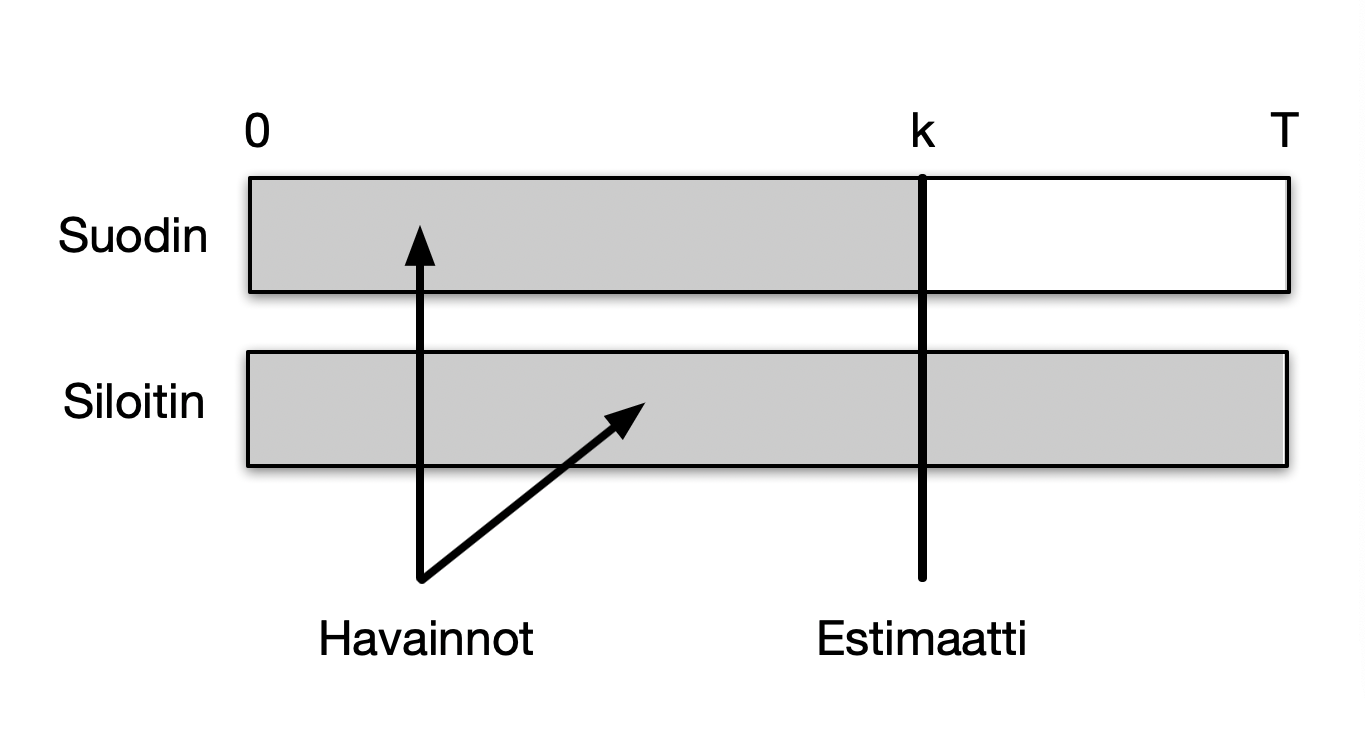
\includegraphics[width=9cm]{suodin_vs_siloitin_cropped}
\caption{Suodin- ja siloitteluongelma}
\label{fig:suodin_vs_siloitin}
\end{figure}

\section{Suodin- ja siloitteluongelmien historiaa}

Tämä alaluku esittää pääpiirteittään suodinongelmalle esitettyjen ratkaisujen historian. Lineaarisen suodinongelman osalta alaluku noudattaa Crisanin artikkelia ``The stochastic filtering problem: a brief historical account'' (2014) \citep{crisan-2014} sekä Grewalin ja Andrewsin artikkelia ``Applications of Kalman Filtering in Aerospace 1960 to the Present'' (2010) \citep{Grewal-2010}. Hiukkassuotimien osalta lähteenä toimii Cappé \&al (2007) \citep{cappe-2007}.

Suodinongelma nousi esille insinööritieteiden sekä sotateollisuuden käytännön ongelmista 2. maailmansodan aikana, vaikkakin suodinongelman diskreetin ajan ratkaisut juontavat jo Andrei N. Kolmogorovin 30-luvun artikkeleihin. Jatkuvan ajan tilanteessa ensimmäisen optimaalisen, kohinan sallivan suotimen esitti kybernetiikan kehittäjä, matemaatikko Norbert Wiener. Wiener-suotimena tunnettua ratkaisuaan varten Wiener muotoili seuraavat kolme ominaisuutta, jotka prosessin \(X_k\) estimaatin \(\hat{X}_k\) pitää toteuttaa.

\begin{enumerate}
\vspace{\baselineskip}
\item \textit{Kausaliteetti}: $X_k$ tulee estimoida käyttäen arvoja $Y_s$, missä $s \leq k$.
\item \textit{Optimaalisuus}: $X_k$:n estimaatin $\hat{X}_k$ tulee minimoida keskineliövirhe $\mathbb{E}[(X-\hat{X}_k)^2]$.
\item \textit{On-line-estimointi}: Estimaatin $\hat{X}_k$ tulee olla saatavissa jokaisella aika-askeleella $k$. 
\vspace{\baselineskip}
\end{enumerate}

Wiener sovelsi ratkaisussaan stationaaristen prosessien spektriteoriaa. Tulokset julkaistiin salaisina Yhdysvaltojen asevoimien tutkimuksesta vastanneen National Defense Research Committeen (NDRC) raportissa vuonna 1942. Tutkimus tunnettiin sodan aikana lempinimellä ``Keltainen vaara'', sekä painopaperinsa värin että vaikeaselkoisuutensa vuoksi. Myöhemmin Wiener esitti tuloksensa julkisesti kirjassaan \textit{Extrapolation, Interpolation and Smoothing of Stationary Time Series} (1949). Wienerin alkuperäiset kolme perusperiaatetta päteveät edelleen kaikille suodinongelman ratkaisuille, myös hiukkassuotimille.

Kenties tärkein ja varmasti tunnetuin lineaariseen suodinongelman ratkaisu on Kalman-suodin. Suotimen kehittivät R.E. Kalman ja R.S. Bucy 1950- ja 60-lukujen taitteessa Yhdysvaltain kylmän sodan kilpavarustelutarpeisiin perustetussa Research Institute for Advanced Studies -tutkimuslaitoksessa (RIAS). Kalman-suodin on suodinongelman diskreetin ajan ratkaisu, kun taas Kalman-Bucy-suodin on jatkuvan ajan ratkaisu. Kohinan ollessa normaalijakautunutta on Kalman-suodin Wiener-suotimen tavoin lineaarisen suodinongelman optimaalinen ratkaisu. Wiener-suotimella ja Kalman-suotimella on kuitenkin erilaiset oletukset, minkä vuoksi erityisesti säätö- ja paikannussovelluksissa Kalman-suotimen käyttö on luontevampaa. Suotimien oletuksia ja oletusten välisiä eroja ei käsitellä tässä tutkielmassa, mutta alaluvussa \ref{kf-yhteydet-erot} käsitellään Kalman-suotimen formaalia yhteyttä hiukkassuotimiin.

Kalman-suodinta voidaan soveltaa myös epälineaarisessa tapauksessa, kunhan suodinongelman funktiot \(f(\cdot)\) ja \(h(\cdot)\) ovat derivoituvia ja niihin liittyvä kohina oletetaan normaalijakautuneeksi. Tätä ratkaisua kutsutaan laajennetuksi Kalman-suotimeksi (\emph{extended Kalman filter}, EKF). Suodin kehitettiin 60-luvulla NASA:n Apollo-ohjelman tarpeisiin, vaikkakin itse avaruusalusten laitteistot hyödynsivät lentoratojen laskennassa Kalman-suotimen perusversiota. Laajennetun Kalman-suotimen toimintaperiaate perustuu epälineaaristen funktioiden linearisointiin Taylorin kehitelmän avulla kulloisenkin estimaatin ympärillä. Laajennettu Kalman-suodin on erityisesti paikannussovellusten \textit{de facto} -suodinstandardi, mutta suodin ei kuitenkaan ole epälineaarisen ongelman optimaalinen estimaattori.

Kalman-suotimesta on lisäksi olemassa lukuisia muita epälineaarisiin ongelmiin soveltuvia laajennuksia, muun muassa paikkaratkaisun Kalman-suodin (\emph{position Kalman filter}, PKF), hajustamaton Kalman-suodin (\emph{unscented Kalman filter}, UKF) sekä tilastollisesti linearisoitu Kalman-suodin (\emph{statistically linearized Kalman filter}, SLF). Kuitenkin jos prosessin \(X_t\) mallia ei tunneta tarkasti tai kohinaa ei voida olettaa normaalijakautuneeksi, ovat hiukkassuotimet eli sekventiaaliset Monte Carlo -menetelmät Kalman-suotimen johdannaisia parempia ratkaisuja. Vaikka tila-avaruuden dimensioiden kasvaessa kasvaa myös hiukkassuotimien vaatima laskentateho, ovat hiukkassuotimet aina sitä parempia mitä epälineaarisempia mallit ovat ja mitä kauempana normaalijakaumasta kohina on. Viimeisten vuosikymmenten aikana laskennan teho on kasvanut merkittävästi samalla kun laskennan hinta on vastaavasti romahtanut, mikä puoltaa Monte Carlo -menetelmien käyttöä entistä useammissa ongelmissa.

Joitakin suodinongelman rekursiivisia Monte Carlo -ratkaisuja löytyy jo 1950\textendash 70-luvuilta, erityisesti säätöteoriaan piiristä. Olennainen nykyalgoritmeihin periytynyt oivallus varhaisissa suodinalgoritmeissa oli tärkeytysotannan käyttö halutun jakaumaestimaatin laskennassa. Tärkeytysotanta-algoritmiin voidaan turvautua, kun emme pysty suoraan tekemään havaintoja jostakin jakaumasta \(p\) ja teemme sen sijaan havaintoja jakaumasta \(q\), jota painotamme niin, että tuloksena saadaan jakauman \(p\) harhaton estimaatti. Algoritmi on kuvattu tarkemmin tutkielman luvussa \ref{hiukkassuotimet}.

Tärkeytysotantaa käyttävä suodinongelman ratkaiseva SIS-algoritmi (\emph{sequential importance sampling}) ei kuitenkaan vielä 70-luvulla löytänyt suurta käytännön suosiota. Osin tämä johtui puutteellisesta laskentatehosta, mutta algoritmi kärsi myös otosten ehtymisenä (\emph{sample impoverishment}) tunnetusta ongelmasta. Monissa ongelmissa SIS-algoritmia käytettäessä suuri osa painoista päätyy vain tietyille partikkeleille, jolloin vastaavasti suuri osa partikkeleista ei enää estimoi haluttua jakaumaa. Tähän ongelmaan palataan myöhemmin tutkielmassa.

Merkittävän ratkaisun ehtymisongelmaan esittivät Gordon, Salmond ja Smith artikkelissaan ``Novel approach to nonlinear/non-Gaussian Bayesian state estimation'' (1993) \citep{Gordon-1993}. Artikkelin ratkaisu kulki nimellä \emph{bootstrap filter}, saapasremmisuodin. Saapasremmisuodin vältti otosten ehtymisen uudellenotannalla, jossa matalapainoiset partikkelit korvattiin otoksilla korkeapainoisemmista partikkeleista. Ratkaisussa painot eivät myöskään riippuneet partikkelien aiemmista poluista vaan ainoastaan havaintojen uskottavuusfunktiosta. Vastaavaa ratkaisua käytetään tämän tutkielman uudemmassa SIR-algoritmissa (\emph{sampling importance resampling}), jossa myös uudelleenotantaan sovelletaan tärkeytysotantaa.

Sekventiaalisissa Monte Carlo -menetelmissä stokastisen prosessin posteriorijakauman esittämiseen käytettyjä otoksia kutsutaan partikkeleiksi tai hiukkasiksi ja menetelmiä siten hiukkassuotimiksi. Erityisesti myöhemmin esitettävää SIR-algoritmia kutsutaan usein hiukkassuotimeksi. Termiä hiukkassuodin käytti ensimmäisen kerran Del Moral artikkelissa ``Nonlinear Filtering: Interacting Particle Resolution'' (1996) \citep{DelMoral-1996}, SMC-menetelmät termiä Liu ja Chen artikkelissa ``Sequential Monte Carlo Methods for Dynamic Systems'' (1998) \citep{Liu-1998}. Tässä tutkielmassa käytetään yleisemmin käytettyä termiä hiukkassuotimet.

\section{Monte Carlo -menetelmistä}

Tässä alaluvussa kuvataan lyhyesti hiukassuotimissa käytettävien Monte Carlo -menetelmien perusperiaate todennäköisyysjakauman estimoinnissa. Lisäksi esitetään tärkeytysotanta-algoritmi (\emph{importance sampling}), jonka tarkoituksena on estimoida harhattomasti jakaumaa \(p(x|y_{1:k})\), josta emme voi suoraan tehdä otoksia, mutta jota voimme approksimoida toisella jakaumalla \(q\). Esitykset noudattavat Särkkää (2013) \citep{sarkka-2013}.

\subsection{Monte Carlo -approksimaatio}

Bayesilaisessa päättelyssä ollaan yleisesti kiinnostuttu laskemaan johonkin posterioritiheysjakaumaan \(p\) liittyvää odotusarvoa

\begin{align}
\mathbb{E}[g(x)|y_{1:k}]=\int g(x)p(x|y_{1:k})dx,
\end{align}

\noindent missä \(g\) on tila-avaruuden mielivaltainen funktio ja \(p(x|y_{1:k})\) on havaintoihin \(\{y_1,\ldots,y_k\}\) liittyvä \(x\):n posterioritiheysjakauma. Odotusarvo on laskettavissa suljetussa muodossa vain harvoissa tapauksissa, suodinongelman kohdalla silloin, kun kyseessä on lineaarinen ja Gaussinen malli. Odotusarvoa voidaan kuitenkin approksimoida niin sanoituilla Monte Carlo -menetelmillä. Menetelmien perusperiaate on tehdä riippumattomia otoksia estimoitavasta jakaumasta ja laskea haluttu odotusarvo otosten avulla. Jos tehdään \(N\) otosta jakaumasta \(x^i\sim p(x|y_{1:k})\), missä \(i=\{1,\ldots,N\}\) saadaan näiden otosten avulla laskettua odotusarvon estimaatti

\begin{align}
\mathbb{E}[g(x)|y_{1:k}]\simeq\frac{1}{N}\sum_{i=1}^N g(x^i).
\end{align}

Monte Carlo -estimaatti konvergoi keskeisen raja-arvolauseen nojalla ja sen estimointivirheen voidaan osoittaa olevan luokkaa \(\mathcal{O}(\frac{1}{\sqrt{N}})\) riippumatta tilamuuttujan \(x\) dimensiosta. Hiukassuotimet hyödyntävät Monte Carlo -estimointia sekventiaalisesti, jolloin estimaatti lasketaan rekursiivisesti kullekin aika-askeleelle \(k=\{1,\ldots, T\}\). Tähän palataan luvuissa \ref{hiukkassuotimet} ja \ref{paikannusesimerkki}.

\subsection{Tärkeytysotanta}

Tilanteessa, jossa Monte Carlo -otoksia ei voida tehdä suoraan jakaumasta \(p\), voidaan hyödyntää jakaumaa \(p\) approksimoivaa tärkeytys- tai ehdotusjakaumaa \(q(x|y_{1:k})\) sekä ns. tärkeytysotantaa. Oletetaan, että tunnetaan priorijakauma \(p(x)\) ja on olemassa havaintomalli \(p(y_{1:k}|x)\) sekä valittu ehdotusjakauma \(q(x|y_{1:k})\), josta voidaan tehdä otoksia. Ehdotusjakaumalta edellytetään lisäksi, että sen kantaja on suurempi tai yhtä suuri kuin jakauman \(p(x|y_{1:k})\) ja että se saa nollasta poikkeavia arvoja kaikkialla missä \(p(x|y_{1:k})\) saa nollasta poikkeavia arvoja. Kirjoitetaan halutun posteriorijakauman odotusarvo integraalina

\begin{align}
\int g(x)p(x|y_{1:k})dx=\int g(x)\frac{p(x|y_{1:k})}{q(x|y_{1:k})}q(x|y_{1:k})dx,
\end{align}

\noindent jolle voidaan muodostaa Monte Carlo -approksimaatio tekemällä \(N\) otosta jakaumasta \(x^i \sim q(x|y_{1:k})\).

Muodostetaan näin odotusarvo

\begin{align}
\mathbb{E}[g(x)|y_{1:k}]\simeq\frac{1}{N}\sum_{i=1}^N\frac{p(x^i|y_{1:k})}{q(x^i|y_{1:k})}g(x^i)=\sum_{i=1}^Nw^ig(x^i),
\end{align}

\noindent missä \(g(x)\) on jokin estimoinnissa hyödyllinen, mielivaltainen funktio. Tutkielmassa käytetty notaatio \(x_k^i\) viittaa aika-askeleen \(k\) partikkeliin \(i\), missä \(i=\{1,\ldots,N\}\). Tärkeytysotantaa kuvaa nyt algoritmi \ref{tarkeytysotanta-algo}. Kun posteriorijakauman estimaatti muodostetaan kyseisellä algoritmilla voidaan tulos kirjoittaa

\begin{align}
\hat{p}(x|y_{1:k})=\sum_{i=1}^{N}w^i \delta(x-x^i),
\end{align}

\noindent missä \(\delta(x)\) on Diracin deltafunktio.

\begin{algorithm}[H]
\label{tarkeytysotanta-algo}
\DontPrintSemicolon
\Begin{
  \For{$i=1,2,\ldots,N$}{
    \Begin{Otetaan $N$ otosta ehdotusjakaumasta $x^i \sim q(x|y_{1:k}).$}
    \Begin{Lasketaan normalisoimattomat painot $w_*^i= p(y_{1:k}|x^i)p(x^i)/q(x^i|y_{1:k}).$ \newline ja normalisoidut painot $w^i=w_*^i/\sum_{j=1}^Nw_*^j$.}
    \Begin{Estimoidaan $p$ laskemalla tiheydelle approksimaatio $\mathbb{E}[g(x)|y_{1:k}]\simeq\sum_{i=1}^Nw^ig(x^i)$.}
    } 
  }  
\caption{Tärkeytysotanta}
\end{algorithm}

\section{Bayesilainen suodin} \label{bayesilainen-suodin}

Suodinongelmassa ollaan kiinnostuttu tilavektorin posteriorijakauman \(p(x_k|y_{1:k})\) estimoinnista. Tässä alaluvussa käydään läpi yleinen rekursiivinen, Bayesilainen posteriorijakauman laskenta. Tällaista suodinongelman ratkaisua kutsutaan myös Bayesilaiseksi suotimeksi. Koska epälineaarisessa, ei-normaalijakautuneessa tilanteessa rekursiota ei voida laskea analyyttisesti, pitää estimoinnissa käyttää numeerisia menetelmiä. Hiukkassuotimissa tämä tarkoittaa jakauman sekventiaalista Monte Carlo -approksimointia ja sen käytännön toteutus esitetään luvun \ref{paikannusesimerkki} algoritmissa. Molemmat esitykset noudattavat Gustafssonia (2010) \citep{gustafsson-2010}.

Bayesilainen ratkaisu tilavektorin posteriorijakauman estimaatille \(\hat{p}(x_k|y_{1:k})\) saadaan seuraavalla rekursiolla (käydään läpi jokaisella aika-askeleella \(k=\{1,\ldots,T\}\)). Lasketaan ensin

\begin{align}\label{bayes-paivitys}
p(x_k|y_{1:k}) = \frac{p(y_k|x_k)p(x_k|y_{1:k-1})}{p(y_k|y_{1:k-1})},
\end{align}

\noindent joka saadaan suoraan Bayesin kaavasta \(\mathbb{P}(A|B)=\mathbb{P}(B|A)\mathbb{P}(A)/\mathbb{P}(B)\). Normalisointivakio lasketaan integraalina

\begin{align}\label{bayes-normalisointi}
p(y_k|y_{1:k-1})=\int_{\mathbb{R}^{n_x}}p(y_k|x_k)p(x_k|y_{1:k-1})\mathop{dx_k},
\end{align}

\noindent joka saadaan kokonaistodennäköisyyskaavasta \(\mathbb{P}(A)=\mathbb{E}[\mathbb{P}(A|X)]=\int_{-\infty}^{\infty}\mathbb{P}(A|X=x)f_X(x)\mathop{dx}\). Merkintä \(\mathbb{R}^{n_x}\) vastaa tässä piilossa olevan tilavektorin dimensiota \(n\).

Lopuksi lasketaan päivitysaskel ajalle, joka saadaan edelleen kokonaistodennäköisyydellä

\begin{align}\label{bayes-aikapaivitys}
p(x_{k+1}|y_{1:k})=\int_{\mathbb{R}^{n_x}}p(x_{k+1}|x_k)p(x_k|y_{1:k})\mathop{dx_k}.
\end{align}

\noindent Rekursion avulla voimme laskea jakauman \(p(x_k|y_{1:k})\) estimaatin käymällä rekursion läpi \(k\) kertaa.

\section{Kalman-suotimen ja hiukkassuotimen yhteydestä ja eroista} \label{kf-yhteydet-erot}

Tässä alaluvussa käsitellään lyhyesti Kalman-suotimen yhteyttä hiukkassuotimeen edellä estitetyn teorian valossa. Esitys noudattaa Särkkää (2013) \citep{sarkka-2013}. Merkitään kuten edellä dynaamista mallia \(x_k\) ja havaintomallia \(y_k\) ja oletataan toisin kuin edellä, että nämä ovat lineaarisia ja noudattavat normaalijakaumaa. Koska mallit ovat lineaarisia, voidaan ne nyt kirjoittaa muotoon

\begin{align}
&\label{kalman-malli1}x_k=\mathbf{A}_{k-1}x_{k-1}+q_{k-1},\\
&\label{kalman-malli2}y_k=\mathbf{H}_k x_k + r_k,
\end{align}

\noindent missä \(\mathbf{A}_{k-1}\) on dynaamisen mallin tilasiirtymään kuvaava matriisi ja \(\mathbf{H}_k\) on havaintojen mallimatriisi. Normaalisuusoletuksesta seuraa, että sekä mallin että prosessin kohinavektorit noudattavat normaalijakaumia \(q_{k-1} \sim \mathcal{N}(0, \mathbf{Q}_{k-1})\) ja \(r_k \sim \mathcal{N}(0, \mathbf{R}_k)\), missä \(\mathbf{Q}_{k-1}\) ja \(\mathbf{R}_k\) ovat kovarianssimatrsiiseja. Lisäksi oletetaan, että prosessin priorijakauma on normaali eli \(x_0 \sim \mathbb{N}(m_0, \mathbf{P_0})\). Mallit voidaan nyt kirjoittaa tiheysfunktiomuodossa

\begin{align}
&\label{kalman-malli-pdf1}p(x_k|x_{k-1})=\mathcal{N}(x_k|\mathbf{A}_{k-1}x_{k-1},\mathbf{Q}_{k-1}),\\
&\label{kalman-malli-pdf2}p(y_k|x_k)=\mathcal{N}(y_k|\mathbf{H}_{k}x_{k},\mathbf{R}_{k}),
\end{align}

\noindent joista voidaan edelleen johtaa suodinongelman mallit

\begin{align}
&\label{kalman-malli-suodin1}p(x_k|y_{1:k-1})=\mathcal{N}(x_k|m_k^* ,\mathbf{P}_k^*),\\
&\label{kalman-malli-suodin2}p(x_k|y_{1:k})=\mathcal{N}(x_k|m_k ,\mathbf{P}_k),\\
&\label{kalman-malli-suodin3}p(y_k|y_{1:k-1})=\mathcal{N}(y_k|\mathbf{H}_k m_k^* ,\mathbf{S}_k)
\end{align}

\noindent ja ongelma ratkaista näin algoritmilla \(\ref{kf}\).

\begin{algorithm}[H]
\label{kf}
\DontPrintSemicolon
\SetAlgoShortEnd
\KwResult{Posteriorijakauman $p(x_{1:k}|y_{1:k})$ estimaatti.\;}
\KwData{Havainnot $y_k$. Priorijakauman $x_0$ keskiarvovektori $m_0$ ja kovarianssimatriisi $\mathbf{P}_0$.\;}
\Begin{
  \For{$k=\{1,2,\ldots,T\}$}{
    \Begin{Ennusteaskel. \newline $m_k^*= \mathbf{A}_{k-1}m_{k-1}$\;}
    \If{$k < t$}{\Begin{Päivitysaskel. \newline $v_k = y_k - \mathbf{H}_k m_k^*$
    \newline $\mathbf{S}_k = \mathbf{H}_k \mathbf{P}_k^* \mathbf{H}_k^\top + \mathbf{R}_k$
    \newline\ $\mathbf{K}_k = \mathbf{P}_k^* \mathbf{H}_k^\top \mathbf{S}_k^{-1}$
    \newline\ $m_k = m_k^* \mathbf{K}_k v_k$
    \newline\ $\mathbf{P}_k = \mathbf{P}_k^* - \mathbf{K}_k \mathbf{S}_k \mathbf{K}_k^\top$;}}
  }  
}
\caption{Kalman-suodin}
\end{algorithm}

Esitetty algoritmi on ns. Kalman-suodin, joka selkeästi toimii suodinongelman ratkaisuna, kun mallit ovat haluttua lineaarista normaalimuotoa. Jos tämä oletus ei täyty, on Kalman-suotimesta kehitetty useita versioita, joissa ei-lineaarinen malli voidaan linearisoida tiettyjen ehtojen vallitessa.

Tämän alaluvun tarkoituksena oli esittää, että Kalman-suotimessa ongelma on samaa muotoa kuin hiukkassuotimessa, joten linearisoituja Kalman-suotimia ei tässä käsitellä. Hiukkassuodin myös ratkaisee suodinongelman mille hyvänsä epälineaariselle mallille.

\chapter{Hiukkassuotimet} \label{hiukkassuotimet}

\section{SIR-algoritmi}

Tässä alaluvussa esitetään epälineaarisen suodinongelman ratkaisemiseksi SIR-hiukkassuodinalgoritmi. Algoritmi on numeerinen toteutus luvussa \ref{bayesilainen-suodin} kuvatusta Bayesilaisesta suotimesta. Esitetty algoritmi perustuu Gustafssoniin (2010) \citep{gustafsson-2010}. Ilman uudelleenotantavaihetta kyseessä olisi SIS-algoritmi.

Algoritmi alustetaan jakaumasta \(x_1^i\sim p_{x_0}\) generoiduilla \(N\) kappaleella partikkeleita. Jokaiselle partikkelille annetaan alustuksessa sama paino \(w_{1|0}^i=1/N\). Algoritmi suoritetaan jokaiselle partikkelille \(i=\{1,2,\ldots,N\}\) jokaisella aika-askeleella \(k=\{1,2,\ldots,T\}\).

Algoritmin ensimmäisessä vaiheessa päivitetään painot yhtälön (\ref{painopaivitys}) mukaan.

\begin{align}\label{painopaivitys}
w^i_{k|k}=\frac{1}{c_k}w^i_{k|k-1}p(y_k|x^i_k).
\end{align}

\noindent Tämä vastaa edellä esitetyn Bayes-suotimen päivitysvaihetta (\ref{bayes-paivitys}). Normalisointipaino \(c_k\) lasketaan puolestaan yhtälöstä (\ref{normalisointi}), mikä vastaa Bayes-suotimen normalisointivakion laskemista (\ref{bayes-normalisointi}) ja asettaa painojen summaksi \(\sum_{i=1}^Nw^i_{k|k}=1\).

\begin{align}\label{normalisointi}
c_k=\sum_{i=1}^{N}w_{k|{k-1}}^ip(y_k|x_k^i).
\end{align}

\noindent Seuraavassa vaiheessa estimoidaan \(p\) laskemalla tiheyden \(p(x_{1:k}|y_{1:k})\) Monte Carlo -estimaatti yhtälön (\ref{p-estimaatti}) perusteella

\begin{align}\label{p-estimaatti}
\hat{p}(x_{1:k}|y_{1:k})=\sum_{i=1}^{N}w_{k|k}^i \delta(x_{1:k}-x_{1:k}^i).
\end{align}

Tämän jälkeen suoritetaan valinnainen uudelleenotanta. Uudelleenotanta voidaan tehdä jokaisella askeleella tai efektiivisen otoskoon perusteella alla kuvatun kynnysarvoehdon \(\hat{N}_{eff}< N_{th}\) täyttessä, jolloin uudelleenotantaa kutsutaan adaptiiviseksi uudelleenotannaksi. Tällaista uudelleenotantaa hyödynnetään esitetyssä algoritmissa (\ref{sir}). Lopuksi päivitetään aika-askel (jos \(k < T\)), luodaan uudet ennusteet partikkeleille ehdotusjakaumasta (\ref{ehdotusjakauma})

\begin{align}\label{ehdotusjakauma}
x_{k+1}^i\sim q(x_{k+1}|x_k^i,y_{k+1})
\end{align}

\noindent ja päivitetään partikkelien painot tärkeytysotannalla (\ref{tarkeytys}) sen mukaan kuinka todennäköisiä partikkelien ennusteet ovat

\begin{align}\label{tarkeytys} w_{k+1|k}^i=w_{k|k}^i\frac{p(x_{k+1}^i|x_k^i)}{q(x_{k+1}^i|x_k^i,y_{k+1})}.
\end{align}

\noindent Vaiheet (\ref{ehdotusjakauma}) ja (\ref{tarkeytys}) vastaavat Bayes-suotimen aikapäivitystä (\ref{bayes-aikapaivitys}).

Alla käsitellään algoritmiin liittyvän uudelleenotantamenetelmän, partikkelien määrän ja ehdotusjakauman valinta. Lopuksi esiteetään algoritmin konvergenssia, marginaalijakaumaa sekä aikakompleksisuutta koskevia tuloksia ja käsitellään algoritmin tuottaman jakaumaestimaatin varianssin estimointia.

\begin{algorithm}[H]
\label{sir}
\DontPrintSemicolon
\SetAlgoShortEnd
\KwResult{Posteriorijakauman $p(x_{1:k}|y_{1:k})$ estimaatti.\;}
\KwData{Havainnot $y_k$. Generoitu $x_1^i\sim p_{x_0}$ missä $i=\{1,\ldots,N\}$ ja jokainen partikkeli saa saman painon $w_{1|0}^i=1/N$.\;}
\Begin{
  \For{$k=\{1,2,\ldots,T\}$}{
    \For{$i=\{1,2,\ldots,N\}$}{
      \Begin{Päivitetään painot $w_{k|k}.$\;}
      \Begin{Estimoidaan $p$ laskemalla tiheydelle approksimaatio $\hat{p}(x_{1:k}|y_{1:k})=\sum_{i=1}^{N}w_{k|k}^i \delta(x_{1:k}-x_{1:k}^i)$.\;}
    }
    \Begin{Lasketaan efektiivinen otoskoko $\hat{N}_{eff}$.\;}
    \If{$\hat{N}_{eff}< N_{th}$}{\Begin{Otetaan uudet $N$ otosta palauttaen joukosta $\{x_{1:k}^i\}_{i=1}^N$, missä otoksen $i$ todennäköisyys on $w^i_{k|k}$.\;}
    \Begin{Asetetaan painot $w^i_{k|k}=1/N$.\;}}
    \If{$k < T$}{\Begin{Aikapäivitys. \newline Luodaan ennusteet partikkeleille ehdotusjakaumasta $x_{k+1}^i\sim q(x_{k+1}|x_k^i,y_{k+1})$, \newline päivitetään partikkelien painot tärkeytysotannalla.\;}}
  }  
}
\caption{SIR}
\end{algorithm}

\subsection{Suunnitteluparametrien valinta}

Ennen algoritmin suorittamista valitaan ehdotusjakauma \(q(x_{k+1}|x_{1:k},y_{k+1})\), uudelleenotantamenetelmä sekä partikkelien määrä \(N\). Ehdotusjakauman ja uudelleenotantamenetelmän valinnassa tärkeimpänä päämääränä on välttää otosten ehtymistä, kun taas partikkelien määrä säätelee kompromissia algoritmin suorituskyvyn ja sen tarkkuuden sekä varianssin välillä.

\subsubsection{Otoskoon $N$ valinta}

Yleispätevää sääntöä otoskoon/partikkelien lukumäärän \(N\) valinnalle on vaikeaa antaa, sillä vaadittava estimointitarkkuus riippuu usein käsillä olevasta ongelmasta. Gordon \&al.~(1993) \citep{Gordon-1993} esittävät kuitenkin kolme tekijää, jotka vaikuttavat partikkelien lukumäärän valintaan

\begin{enumerate}
\def\labelenumi{\alph{enumi}.}
\tightlist
\item
  tila-avaruuden ulottuvuuksien lukumäärä \({n_x}\),
\item
  tyypillinen päällekäisyys priorin ja uskottavuuden välillä
\item
  sekä tarvittava aika-askelten lukumäärä.
\end{enumerate}

Ensimmäisen tekijän vaikutus on selvä. Mitä useammassa ulottuvuudessa otantaa tarvitsee tehdä, sen korkeammaksi on \(N\) asetettava, jotta jokainen ulottuvuus pystytään kattamaan tehokkaasti. Tekijät (\textit{b}) ja (\textit{c}) puolestaan seuraavat uudelleenotannasta. Jos se osa tila-avaruutta, jossa uskottavuus \(p(y_k|x_k)\) saa merkittäviä arvoja on pieni verrattuna siihen osaan, jossa priorijakauma \(p(x_k|y_{1:k-1})\) saa merkittäviä arvoja, suuri osa partikkeleista saa pieniä painoja eikä näin valikoidu uudelleenotantaan.

Yleisesti ottaen \(N\) kannattaa asettaa sellaiseksi, että se paitsi tuottaa riittävän tarkan estimaatin, on se myös käytettävissä olevan laskentatehon sekä vaadittavan laskentanopeuden kannalta järkevä. Tähän palataan tutkielman empiirisessä paikannusesimerkissä.

\subsubsection{Uudelleenotantamenetelmän valinta} \label{uudelleenotantamenetelman-valinta}

Ilman uudelleenotantaa on mahdollista, että algoritmi alkaa kärsiä SIS-algoritmille tyypillisestä otosten ehtymisestä. Toisin sanoen kaikki painot alkavat keskittyä vain muutamalle partikkelille eikä algoritmi enää approksimoi tehokkaasti haluttua jakaumaa. Uudelleenotanta tarjoaa osittaisen ratkaisun tähän ongelmaan, mutta hävittää samalla informaatiota ja lisää siten satunnaisotantaan liittyvää epävarmuutta. Yleisesti ottaen uudelleenotanta kannattaa aloittaa vasta siinä vaiheessa algoritmin suorittamista, kun siitä on otosten ehtymisen kannalta hyötyä, esimerkiksi efektiivisen otoskoon pudottua jonkin kynnysarvon alapuolelle (adaptiivinen uudelleenotanta). Efektiivinen otoskoko saadaan laskettua variaatiokertoimesta \(c_\nu\) kaavalla

\begin{align}\label{N-eff}
N_{eff}= \frac{N}{1+c_\nu^2(w^i_{k|k})} = \frac{N}{1+\frac{\text{Var}(w^i_{k|k})}{(\mathbb{E}[w^i_{k|k}])^2}} =\frac{N}{1+N^2\text{Var}(w^i_{k|k})}.
\end{align}

Näin laskettu efektiivinen otoskoko maksimoituu (\(N_{eff}=N\)), kun kaikille painoille pätee \(w^i_{k|k}=1/N\) ja minimoituu (\(N_{eff}=1\)), kun \(w^i_{k|k}=1\) todennäköisyydellä \(1/N\) ja \(w^i_{k|k}=0\) todennäköisyydellä \((N-1)/N\). Normalisoitujen painojen avulla saadaan efektiiviselle otoskoolle aika-askeleella \(k\) laskennallinen approksimaatio

\begin{align}\label{N-hat-eff}
\hat{N}_{eff}=\frac{1}{\sum_{i=1}^N(w^i_{k|k})^2}.
\end{align}

Määritelmille (\(\ref{N-eff}\)) ja (\(\ref{N-hat-eff}\)) pätee \(1 \leq \hat{N}_{eff} \leq N\). Yläraja saavutetaan, kun jokaisen partikkelin paino on sama. Alarajalle päädytään, kun kaikki paino keskittyy yksittäiselle partikkelille. Tästä saadaan määriteltyä algoritmille SIR-uudelleenotantaehto \(\hat{N}_{eff}< N_{th}\). Gustafsson (2010) \citep{gustafsson-2010} esittää uudelleenotannan kynnysarvoksi esimerkiksi \(\hat{N}_{th}=2N/3\).

Uudelleenotanta ei muuta approksimoitavan jakauman \(p\) odotusarvoa, mutta se lisää jakauman Monte Carlo -varianssia. On kuitenkin olemassa esimerkiksi osittamiseen perustuvia uudelleenotantamenetelmiä, jotka pyrkivät minimoimaan varianssin lisäyksen. Varianssin pienennysmenetelmät jätetään tämän tutkielman ulkopuolelle.

\subsubsection{Ehdotusjakauman valinta}

Yksinkertaisin muoto ehdotusjakaumalle on \(q(x_{1:k}|y_{1:k})\) eli jokaisella algoritmin suorituskerralla käydään läpi koko aikapolku \(1\):\(k\). Tämä ei kuitenkaan ole tarkoituksenmukaista, erityisesti jos kyseessä on reaaliaikainen sovellutus. Kirjoitetaan sen sijaan ehdotusjakauma muodossa

\begin{align}\label{proposal-factorization}
q(x_{1:k}|y_{1:k})=q(x_k|x_{1:k-1},y_{1:k})q(x_{1:k-1}|y_{1:k}).
\end{align}

Jos yhtälöstä (\ref{proposal-factorization}) poimitaan ehdotusjakaumaksi ainoastaan termi \(q(x_k|x_{1:k-1},y_{1:k})\), voidaan tämä kirjoittaa edelleen Markov-ominaisuuden nojalla muotoon \(q(x_k|x_{k-1},y_{k})\). Tämä on suodinongelman kannalta riittävää, koska olemme kiinnostuneita posteriorijakaumasta ja arvosta \(x\) ainoastaan aika-askeleella \(k\) (siloitinongelmassa tarvitsisimme koko polun \(x_{1:k}\)). Alla tarkastellaan edelleen Gustafssonia (2010) \citep{gustafsson-2010} seuraten kahta ehdotusjakauman valintatapaa, prioriotantaa (\emph{prior sampling}) sekä uskottavuusotantaa (\emph{likelihood sampling}).

Ennen ehdotusjakauman tarkastelua määritellään mallille signaali-kohinasuhde uskottavuuden maksimin ja priorin maksimin välisenä suhteena

\begin{align}\label{SNR}
\text{SNR}\propto \frac{\text{max}_{x_k}p(y_k|x_k)}{\text{max}_{x_k}p(x_k|x_{k-1})}. 
\end{align}

\noindent Yhdistetään lisäksi ehdotusjakaumia varten yhtälöt (\ref{painopaivitys}) ja (\ref{normalisointi}), jolloin saadaan painojen päivitys muotoon

\begin{align}\label{painopaivitys-propto}
w^i_{k|k} \propto w^i_{k-1|k-1}\frac{p(y_k|x^i_k)p(x_k|x^{k-1})}{q(x_k|x^i_{k-1},y_k)}.
\end{align}

Kun suhde (\ref{SNR}) on matala, on prioriotanta luonnollinen valinta. Tässä käytetään ehdotusjakaumana tilavektorin ehdollista prioria eli

\begin{align}\label{prioriotanta-q}
q(x_k|x_{1:k-1},y_{k})=p(x_k|x^i_{k-1}).
\end{align}

\noindent Yhtälön (\ref{prioriotanta-q}) perusteella saadaan edelleen prioriotannan painoiksi

\begin{align}\label{prioriotanta-w}
w^i_{k|k} = w^i_{k|k-1}p(y_k|x^i_k) = w^i_{k-1|k-1}p(y_k|x^i_k).
\end{align}

Kun signaali-kohinasuhde on kohtalainen tai korkea, on parempi käyttää ehdotusjakaumana skaalattua uskottavuusfunktiota (\ref{uskottavuusotanta-q}). Tarkastellaan ensin tekijöihin jakoa

\begin{align}\label{uskottavuusotanta-factorization}
p(x_k|x^i_{k-1},y_k)=p(y_k|x_k)\frac{p(x_k|x^i_{k-1})}{p(y_k|x^i_{k-1})}.
\end{align}

\noindent Kun SNR on korkea ja uskottavuusfunktio on integroituva pätee \(p(x_k|x^i_{k-1},y_{k}) \propto p(y_k|x_k)\), jolloin voidaan asettaa

\begin{align}\label{uskottavuusotanta-q}
q(x_k|x^i_{k-1},y_{k}) \propto p(y_k|x_k).
\end{align}

\noindent Yhtälön (\ref{uskottavuusotanta-q}) perusteella saadaan edelleen uskottavuusotannan painoiksi

\begin{align}\label{uskottavuusotanta-w}
w^i_{k|k} = w^i_{k-1|k-1}p(x^i_k|x^i_{k-1}).
\end{align}

\subsection{Konvergenssituloksia}

Alla esitetään kolme SIR-algoritmiin liittyvää konvergenssitulosta. Se, kuinka hyvin esitetyllä algoritmilla arvioitu posterioritiheys \(\hat{p}(x_{1:k}|y_{1:k})\) approksimoi todellista tiheysfunktiota \(p(x_{1:k}|y_{1:k})\), se mikä on approksimaation keskineliövirhe sekä keskeinen raja-arvolause. Tulokset 1\textendash 2 noudattavat Crisanin ja Doucet'n artikkeleita ``Convergence of Sequential Monte Carlo Methods'' (2000) \citep{crisan-2000} ja ``A Survey of Convergence Results on Particle Filtering Methods for Practitioners'' (2002) \citep{crisan-2002}, tulos 3 Chopinin artikkelia ``Central limit theorem for sequential Monte Carlo methods and its application to Bayesian inference'' (2004) \citep{chopin-2004}.

\textit{Konvergenssitulos 1}: Kun \(N \to \infty\) algoritmille pätee kaikille aika-askeleille \(k\) tulos (\ref{jakaumakonvergenssi}).

\begin{align}\label{jakaumakonvergenssi}
\hat{p}(x_{1:k}|y_{1:k}) \xrightarrow{a.s.} p(x_{1:k}|y_{1:k}).
\end{align}

\textit{Konvergenssitulos 2}: Keskineliövirheelle pätee asymptoottinen konvergenssi (\ref{MSE-konvergenssi}).

\begin{align}\label{MSE-konvergenssi}
\mathbb{E}\left[\hat{g}(x_k)-\mathbb{E}\left[g(x_k)\right]\right]^2\leq\frac{p_k\norm{g(x_k)}}{N},
\end{align}

\noindent missä \(g\) on mikä hyvänsä piilossa olevan tila-avaruuden rajoitettu Borel-mitallinen funktio (\(g \in \mathcal{B}(\mathbb{R}^{n_x})\)), \(\norm{g(\cdot)}\) kyseisen funktion supremum-normi ja \(p_k\) jokin äärellinen vakio, jolle pätee ajanhetkestä \(k\) riippumatta \(p_k=p<\infty\).

\textit{Konvergenssitulos 3}: Keskeinen raja-arvolause (\ref{CLT}).

\begin{align}\label{CLT}
\text{Kun } N \to \infty: \sqrt{N} \left\{ \frac{1}{N} \sum_{i=1}^N \hat{g}(x_k^i) -\mathbb{E}\left[g(x_k^i)\right] \right\} \xrightarrow{D} \mathcal{N}(0,\sigma^2 < \infty),
\end{align}

\noindent missä \(g\) on jälleen mikä hyvänsä piilossa olevan tila-avaruuden rajoitettu Borel-mitallinen funktio (\(g \in \mathcal{B}(\mathbb{R}^{n_x})\)). Konvergenssituloksia ei tämän tutkielman puitteissa todisteta.

\subsection{Marginaalijakauma}

Edellä kuvattu algoritmi \ref{sir} tuottaa approksimaation koko prosessin posteriorijakaumalle \(p(x_{1:k}|y_{1:k})\). Jos halutaan tietää ainoastaan posteriorijakauman \(p(x_k|y_{1:k})\) estimaatti, voidaan käyttää yksinkertaisesti viimeisestä tilasta \(x_k\) laskettua estimaattia

\begin{align}
\hat{p}(x_{k}|y_{1:k})=\sum_{i=1}^{N}w_{k|k}^i \delta(x_{k}-x_{k}^i).
\end{align}

Toinen, tarkempi vaihtoehto on käyttää laskennassa tärkeytyspainoa

\begin{align}\label{marginaalitarkeytys}
w_{k+1|k}^i=\frac{\sum_{j=1}^{N}w_{k|k}^jp(x_{k+1}^i|x_k^j)}{q(x_{k+1}^i|x_k^i,y_{k+1})}
\end{align}

\noindent painon (\ref{tarkeytys}) sijaan. Tällöin jokaisella aikapäivitysaskeleella lasketaan painot kaikkien mahdollisten tila-aika-avaruuspolkujen yli. Samoin kuin uudelleenotanta tämä pienentää painojen varianssia, mutta lisää algoritmin aikakompleksisuutta.

\subsection{Aikakompleksisuus}

Algoritmin perusmuodon aikakompleksisuus on \(\mathcal{O}(N)\). Uudelleenotantamenetelmän tai ehdotusjakauman valinta ei suoraan vaikuta aikakompleksisuuteen. Sen sijaan marginalisointi tärkeytyspainolla (\ref{marginaalitarkeytys}) lisää algoritmin aikakompleksisuutta \(\mathcal{O}(N)\rightarrow\mathcal{O}(N^2)\), koska jokaisen partikkelin kohdalla painot lasketaan jokaisen tila-aika-avaruuspolun yli. On selvää, että erityisesti isoilla otoskoon \(N\) arvoilla ei yllä esitetty marginalisointi enää ole mielekästä.

Tällaisia tilanteita varten algoritmista on olemassa \(\mathcal{O}(N\text{log}(N))\)-versioita, jotka perustuvat esimerkiksi N:n kappaleen oppimiseen (\emph{N-body learning}). Näiden algoritmien käsittely jää tämän tutkielman ulkopuolelle, mutta katsauksen algoritmeista ovat esittäneet esimerkiksi Klaas \&al.~artikkelissa ``Toward Practical \(N^2\) Monte Carlo: the Marginal Particle Filter'' (2005) \citep{klaas-2005}.

\section{Saapasremmisuodin}

Saapasremmisuodin \ref{saapasremmisuodin} eli \emph{bootstrap filter} on SIR-algoritmin muunnelma, jossa tärkeytysotannanssa (kts. \ref{tarkeytysotanta-algo}) käytetään dynaamista mallia \(p(x_k|x_{k-1})\).

\begin{algorithm}[H]
\label{saapasremmisuodin}
\DontPrintSemicolon
\SetAlgoShortEnd
\KwResult{Posteriorijakauman $p(x_{1:k}|y_{1:k})$ estimaatti.\;}
\KwData{Havainnot $y_k$. Generoitu $x_1^i\sim p_{x_0}$ missä $i=\{1,\ldots,N\}$ ja jokainen partikkeli saa saman painon $w_{1|0}^i=1/N$.\;}
\Begin{
  \For{$k=\{1,2,\ldots,T\}$}{
    \For{$i=\{1,2,\ldots,N\}$}{
      \Begin{Luodaan uudet estimaatit dynaamisesta mallista $x_{k}^i\sim p(x_{k}|x_{k-1}^i)$.;}
      \Begin{Päivitetään hiukkasten painot $w_k^i$ uskottavuusfunktion $p(y_k|x_k^i)$ mukaan.}
      \Begin{Estimoidaan $p$ laskemalla tiheydelle approksimaatio $\hat{p}(x_{1:k}|y_{1:k})=\sum_{i=1}^{N}w_{k|k}^i \delta(x_{1:k}-x_{1:k}^i)$.}
    }
    \If{$k < t$}{\Begin{Aikapäivitys. Suoritetaan uudelleenotanta kuten SIR-algoritmissa \ref{sir}.\;}}
  }  
}
\caption{Saapasremmisuodin}
\end{algorithm}

Saapasremmisuodin on edellä esitettyä SIR-algoritmia yksinkertaisempi toteuttaa, mutta epäinformatiivisen tärkeytysjakauman vuoksi algoritmi saattaa vaatia SIR-algoritmia suuremman määrän hiukkasia. Saapasremmisuodin esitetään tässä sen historiallisen tärkeyden vuoksi, sillä kyseessä oli ensimmäinen uudelleenotataantaa hyödyntävä hiukkassuodinalgoritmi. Suotimien käytännön toteutukseen palataan luvussa \ref{paikannusesimerkki}.

\section{Varianssin estimoinnista} \label{varianssin-estimointi}

Hiukkassuotimen varianssin estimoinnissa ollaan kiinnostuneita jakaumaestimaatin \(\hat{p}(x_{1:k}|y_{1:k})\) varianssista. Yksinkertaisin tapa estimoida hiukkassuodinalgoritmin varianssia on ajaa algoritmi \(M > 1\) kertaa. Koska ajot ovat toisistaan riippumattomia, voidaan estimaatin varianssi laskea kullekin aika-askeleelle \(k\) näiden ajojen \(k\)-hetken estimaattien otosvarianssina:

\begin{align}\label{MC-varianssi}
\hat{\sigma}^2_{MC} = \text{Var}(\hat{p}(x_{1:k}|y_{1:k})) = \frac{1}{M-1} \sum_{i=1}^{M}(x_k^i-\bar{x}_k)^2
,\end{align}

\noindent missä \(x_k^i\) on \(k\):nen aika-askeleen piste-estimaatti ajolle \(i=1,\ldots,M\) ja \(\bar{x}_k\) piste-estimaattien aritmeettinen keskiarvo laskettuna kaikkien \(M\) ajon yli. Tällaisen Monte Carlo -varianssin estimoiminen on kuitenkin laskennallisesti tehotonta. Monissa käytännön sovellutuksissa jo yhden hiukkassuodinalgoritmin ajaminen vaatii runsaasti laskentatehoa, jolloin Monte Carlo -varianssin laskeminen ei ole mahdollista.

Varianssia ei voida myöskään laskea analyyttisesti, mutta koska keskeisen raja-arvolauseen (\ref{CLT}) nojalla tiedetään, että asymptoottinen varianssi

\begin{align}\label{asymptoottinen-varianssi}
\lim_{N\to \infty} N \text {Var}(\hat{g}(x_k^i))
\end{align}

\noindent on olemassa, on sen estimointiin kehitetty lähivuosina joitakin approksimatiivisia menetelmiä. Alla käsitellään Chan ja Lain (2013) \citep{Chan-2013} sekä Leen ja Whitleyn (2018) ehdottamaa varianssin estimointitapaa \citep{Lee-2018}.

Ajetaan SIR-algoritmi kuten esitetty algoritmissa \ref{sir}, mutta merkitään kullakin aika-askeleella \(k=1,\ldots,T\) jokaisen partikkelin \(n=1,\ldots,N\) kohdalla indeksillä \(E_k^n\) kunkin partikkelin kantaisää eli sitä partikkelia, josta kyseinen partikkeli on uudelleenotantojen kautta polveutunut aika-askeleesta \(k=1\) lähtien. Kaavio \ref{fig:eeva-indeksit} havainnollistaa tätä partikkelien polveutumista.

\begin{figure}[H]
\centering
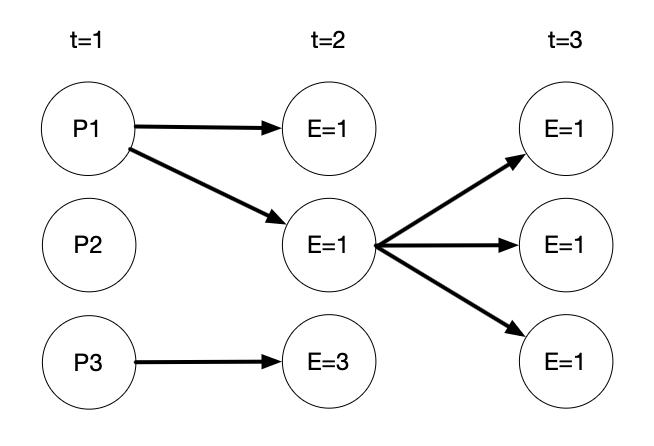
\includegraphics[width=9cm]{eevaindeksit}
\caption{Esimerkki Eeva-indekseistä, kun $T=3$ ja $N=3$.}
\label{fig:eeva-indeksit}
\end{figure}

Varianssiestimaatti voidaan laskea näiden, Leen ja Whitleyn Eeva-indekseiksi nimeämien indeksien perusteella seuraavasti. Merkitään ensin Eeva-indekseillä painotettua summaa

\begin{align}\label{CLE-sum}
\hat{\mu}_k=\sum_{i=1}^N w_k^i x_k^i[E_k]
,\end{align}

\noindent missä merkintä \(x_k^i[E_k]\) tarkoittaa, että partikkeleista \(x_k\) valitaan Eeva-indeksien osoittamat partikkelit eli ne partikkelit joille \(i=E_k^j\), kun \(j=1,\ldots,N\). Sama partikkeli voidaan luonnollisesti valita summaan useamman kerran. Tämän perusteella lasketaan edelleen varianssi

\begin{align}\label{CLE-varianssi}
\hat{\sigma}^2_{CLE} = \frac{1}{N(N-1)} \sum_{i=1}^N w_k^i (x_k^i[E_k]-\hat{\mu}_k)^2
.\end{align}

\noindent Kyseessä harhaton ja konsistentti asymptoottisen varianssin estimaatti. Tarkemmin \(N\hat{\sigma}^2_{CLE}\) konvergoi asymptoottiseen varianssiin (\ref{asymptoottinen-varianssi}). Tätä ei tutkielman puitteissa todisteta.

Yllä esitetty varianssiestimaatti saattaa kuitenkin kärsiä indeksien ehtymisestä. Toisin sanoen kun \(k \to \infty\), polveutuvat kaikki hiukkaset lopulta samasta kantaisästä eli indeksit \(E_k^i,\ldots,E_k^N\) ovat kaikki yhtäsuuria. Tämän vuoksi on mielekästä johtaa indeksit ainoastaan tietystä aiemmasta aika-askeleesta aika-askeleen \(k=1\) sijaan. Olsson ja Douc (2019) \citep{olsson-2019} ehdottavat tähän tarkoitukseen Henok-indeksiä \(E_{m,k}^n\), jossa \(m\) merkitsee aika-askeleen \(m\leq k\) partikkelia, josta kyseinen partikkeli polveutuu. Partikkelien kantaisien sukupolvi määritetään viipeellä \(\lambda\) niin, että \(m=k-\lambda\). Kaavio \ref{fig:henok-indeksit} havainnollistaa partikkelien polveutumista, kun \(\lambda=1\).

\begin{figure}[H]
\centering
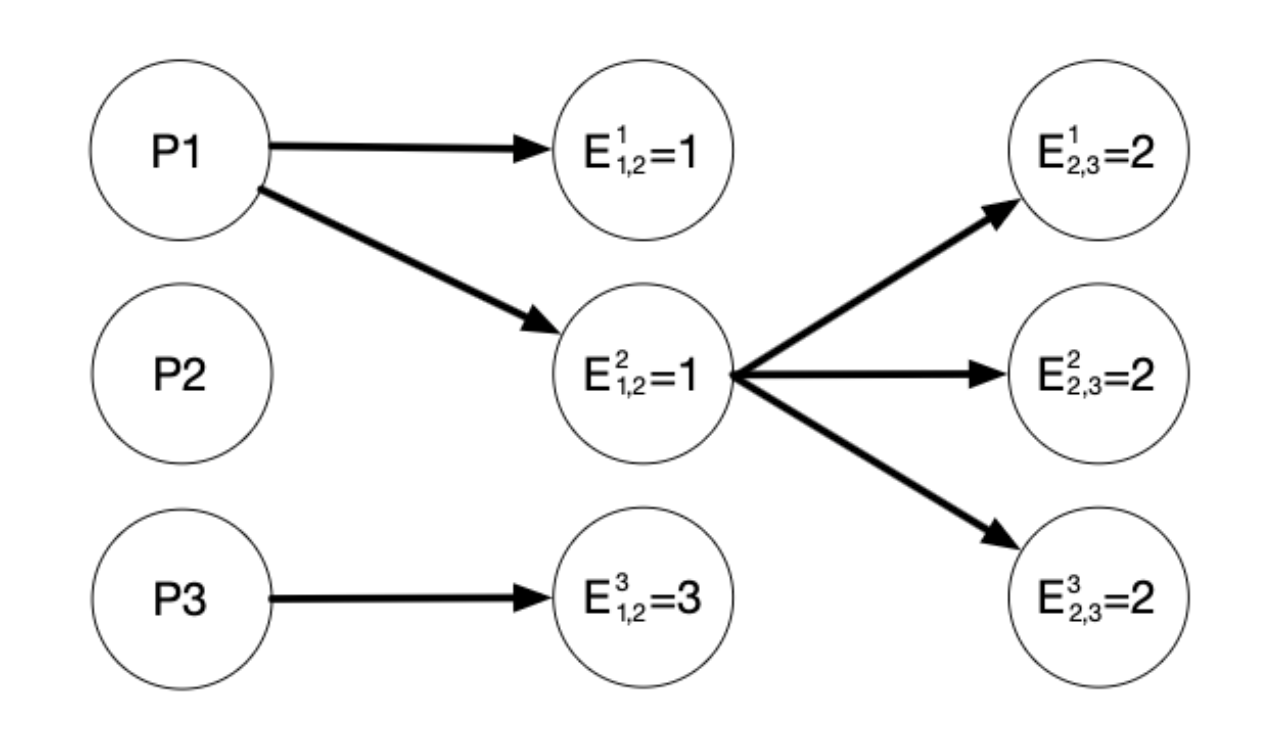
\includegraphics[width=9cm]{henokindeksit_korjattu}
\caption{Esimerkki Henok-indekseistä, kun $T=3$, $N=3$ ja $\lambda=1$.}
\label{fig:henok-indeksit}
\end{figure}

Nyt varianssi voidaan laskea kuten yhtälössä (\ref{CLE-varianssi}) edellä, mutta Eeva-indeksit korvataan Henok-indekseillä. Saadaan painotettu summa

\begin{align}\label{OD-sum}
\hat{\mu}_k=\sum_{i=1}^N w_k^i x_k^i[E_{k(\lambda)}]
\end{align}

\noindent ja varianssi

\begin{align}\label{OD-varianssi}
\hat{\sigma}^2_{OD} = \frac{1}{N-1} \sum_{i=1}^N w_k^i (x_k^i[E_{k(\lambda)}]-\hat{\mu}_k)^2
,\end{align}

\noindent missä \(k(\lambda) \vcentcolon= k-\lambda\) eli se aika-askel, jota käytetään hiukkasten kantaisänä. Viive \(\lambda\) on varianssiestimaatin suunnitteluparametri. Pienillä viipeillä estimaatti on harhainen, mutta harha laskee viipeen kasvaessa. Olsson ja Douc suosittavat viipeen ylärajaksi arvoa \(\lambda=20\), jolloin estimaattorin harha on käytännössä kokonaan hävitetty. Tätä suuremmilla viivearvoilla estimaatti voi alkaa kärsiä samasta epätarkkuudesta kuin Eeva-indekseihin perustuva CLE-estimaatti.

Mastrototaro ja Olsson (2023) \citep{Mastrototaro-2023} laajentavat estimaattia edelleen niin, että viive \(\lambda\) valitaan mukautuvasti. Mastrototaron ja Olssonin ALVar-estimaatti (\emph{Adaptive-Lag Variance}) lasketaan kuten OD-varianssi (\ref{OD-varianssi}) edellä, mutta kunkin algoritmin ajokerran jälkeen asetetaan seuraavan ajanhetken \(\lambda\) seuraavasti:

\begin{align}\label{ALVar-lambda}
\lambda_{k+1} \leftarrow \operatorname*{arg\,max}_{\lambda \in [0, \lambda_k + 1]} \hat{\sigma}^2_{k+1,\lambda}
\end{align}

\noindent ja ehtyneet Henok-indeksit määritellään niin, että indeksi on ehtynyt (so. kaikki indeksivektorin indeksit ovat yhtäsuuria), jos jompikumpi seuraavista ehdoista täyttyy:

\hfill\break
i) Henok-indeksit \(E^i_{m,k-1}\) ovat ehtyneet,\\
ii) Henok-indeksit \(E^i_{m-1,k}\) ovat ehtyneet ja on olemassa \(\lambda^\prime \in [0, \lambda-1]\), joka täyttää ehdon \(\hat{\sigma}^2_{k+1,\lambda} < \hat{\sigma}^2_{k+1,\lambda^\prime}\), koska myös ehtyneiden indeksien kantaisät ovat ehtyneitä.\\

Nyt indeksi \(\lambda_{k+1}\) voidaan valita rekursiivisesti niin, että se tuottaa suurimman varianssiestimaatin, joka on kuitenkin rajoitettu ylhäältä arvoon \(\lambda_k+1\). Tämä indeksi ei ole koskaan ehtynyt, joten se on myös parhaan varianssiestimaatin tuottava valinta.

Esitettyjä varianssiestimaatteja voidaan hyödyntää paitsi algoritmien ja parametrivalintojen vertailussa myös mukautuvan viipeen hiukkassiloittimen viipeen valinnassa (kts. luku \ref{hiukkassiloittimet}). Varianssiestimaatti lasketaan myös luvun \ref{paikannusesimerkki} empiirisessä esimerkissä.

\chapter{Hiukkassilottimet} \label{hiukkassiloittimet}

Tässä luvussa käsitellään suodinongelmaan läheisesti liittyvän siloitteluongelman ratkaisemista hiukkassiloitinalgoritmien avulla. Kuten hiukkassuotimien kohdalla, myös tässä luvussa esitetään ongelma ensin yleisessä Bayesilaisessa muodossa, jonka jälkeen siirrytään käsittelemään hiukkasmenetelmiin pohjautuvia siloitinalgoritmeja. Luvussa käsiteltävät algoritmit jaetaan kahteen pääkategoriaan, offline-algoritmeihin, joita sovelletaan hiukkassuodinalgoritmin ajon jälkeen ja online-algoritmeihin, jotka suoritetaan hiukkassuodinalgoritmin rinnalla.

Siloitinongelman esittely seuraa Särkkää (2013) \citep{sarkka-2013}. Algoritmien käsittely pohjautuu SIR- ja BS-PS-siloittimien osalta Särkkään (2013) \citep{sarkka-2013} ja SIR-siloittimen osalta Kitagawan artikkeliin ``Monte Carlo filter and smoother for non-Gaussian nonlinear state space models'' (1996) \citep{kitagawa-1996}. Kiinteän viipeen silotin seuraa niin ikään Kitagawaa (1996) \citep{kitagawa-1996}. Uudelleenpainottava siloitin perustuu Doucetin \&al.~artikkeliin ``On sequential Monte Carlo sampling methods for Bayesian filtering'' (2000) \citep{Doucet-2000}. Mukautuvan viipeen siloitin seuraa puolestaan Alenlövin ja Olssonin artikkelia ``Particle-Based Adaptive-Lag Online Marginal Smoothing in General State-Space Models'' (2019) \citep{alenlov-2019}.

\section{Bayesilainen siloitin}

Bayesilaisen siloittimen tarkoitus on laskea tilan \(x_k\) marginaaliposteriorijakauma \(p(x_k|y_{1:T})\) aika-askeleella \(k\), kun käytössä on havaintoja aika-askeleeseen \(T\) asti, missä \(T>k\). Ero Bayesilaiseen suotimeen (kts. alaluku \ref{bayesilainen-suodin}) on siinä, että suodinongelmassa havaintoja on saatavilla ainoastaan aika-askeleeseen \(k\) asti, kun taas siloitinongelmassa myös tulevat havainnot ovat saatavilla. Ajassa taaksepäin etenevät rekursiiviset yhtälöt ongelman ratkaisemiseksi voidaan esittää muodossa

\begin{align}\label{siloitin-prediktiivinen}
p(x_{k+1}|y_{1:k})=\int_{\mathbb{R}^{n_x}}p(x_{k+1}|x_k)p(x_k|y_{1:k})\mathop{dx_k}
\end{align}

ja

\begin{align}\label{siloitin-ratkaisu}
p(x_k|y_{1:T}) = p(x_k|y_{1:k}) \int \frac{p(x_{k+1}|x_k)p(x_{k+1}|y_{1:T})}{p(x_{k+1}|y_{1:k})} \mathop{dx_{k+1}},
\end{align}

\noindent missä \(p(x_k|y_{1:k})\) on suodintiheys aika-askeleella \(k\) ja \(p(x_{k+1}|y_{1:k})\) prediktiivinen jakauma ajanhetkelle \(k+1\). Kuten suodinongelman kohdalla, voidaan ongelma ratkaista suljetussa muodossa, kun mallit ovat lineaarisia. Tällöin kyseessä on Rauch-Turn-Striebel-siloitin (RTSS), josta käytetään myös nimitystä Kalman-siloitin. Samoin kuten Kalman-suotimen kohdalla, ongelma voidaan tiettyjen ehtojen vallitessa linearisoida. Näitä linearisoituja siloittimia ei käsitellä tässä tutkielmassa. Hiukkassuotimen tavoin hiukkassiloitin ratkaisee siloitteluongelman mille hyvänsä epälineaariselle mallille.

\section{Offline-algoritmit}

Tässä alaluvussa käsitellään lyhyesti muutamaa ehdotettua offline-hiukkassiloitinalgoritmia. Offline-siloittimet estimoivat siloitintiheyttä aika-askeleella \(k<T\), kun havaintodata on käytössä koko ajanjaksolta \(1 \ldots T\). Alla esitetyt algoritmit siis olettavat, että kaikki mahdollinen tuleva data on jo niiden käytössä.

\subsection{SIR-siloitin}

Kuten aiemmin mainittua, näyttävät hiukkassuodinalgoritmit, erityisesti SIR-algoritmi \ref{sir}, ratkaisevan siloitteluongelman ilmaiseksi, kunhan tallennamme aika-askeleella \(k\) koko otoshistorian \(x_{0:k}^i\). Tällöin voimme estimoida täyttä siloitteluposteriorijakaumaa seuraavasti:

\begin{align}\label{siloitin-posteriori}
p(x_{0:T}|y_{1:T}) \approx \sum_{i=1}^N w_T^i \delta (x_{0:T}-x_{0:T}^i).
\end{align}

Nyt aika-askeleen \(k\) siloitinjakauma saadaan laskettua

\begin{align}\label{siloitin-posteriori-k}
p(x_{k}|y_{1:T}) \approx \sum_{i=1}^N w_T^i \delta (x_{k}-x_{k}^i),
\end{align}

\noindent missä \(x^i_k\) on \(x^i_{0:T}\):n \(k\):s elementti. Koska uudelleenotanta hävittää otoshistorian, pitää uudelleenotanta suorittaa koko otoshistoriasta \(x_{0:k}^i = (x_{0:k-1}^i, x_{k}^i)\) pelkän aika-askeleen \(k\) otoksen \(x_{k}^i\) sijaan. Koska nyt koko otoshistoria pitää tallentaa, vaatii SIR-siloitin \(NkT\) muistia \(N\) sijaan. Vastaavasti myös uudelleenotannan aikakompleksisuus kasvaa \citep{kitagawa-1996}.

SIR-siloittimen suurin ongelma on kuitenkin sen tuottamien estimaattien epätarkkuus. Kun aika-askeleiden määrä kasvaa, johtaa koko otoshistorian uudelleenotanta kaiken painon kasautumiseen historian tietyille otoksille, jolloin SIR-siloittimen tuottamat estimaatit eivät enää estimoi haluttua (siloittelu)posteriorijakaumaa \citep{kitagawa-1996}.

\subsection{BS-PS-siloitin}

\emph{Backward-simulation particle smoother} (BS-PS) eli taaksepäin simuloiva hiukkassiloitin estimoi hiukkassuotimen tulosten perusteella tehokkaammin siloitinjakaumaa. Tässä algoritmissa hiukkasten historia simuloidaan aika-askeleesta \(T\) taaksepäin ensimmäiseen aika-askeleeseen:

\begin{algorithm}[H]
\label{BSPS}
\DontPrintSemicolon
\SetAlgoShortEnd
\KwResult{Posteriorisiloitinjakauman $p(x_{k}|y_{1:T})$ estimaatti.\;}
\KwData{Suodinjakaumia edustavat hiukkaset ja näihin liittyvät painot ${w_k^i, x_k^i}$, missä $i=1,\ldots,N$ ja $k=1,\ldots,T$.\;}
\Begin{
  \Begin{Valitaan $\tilde{x}_T=x_T^i$\;}
  \For{$k=\{T-1,\ldots,0\}$}{
    \Begin{Lasketaan uudet painot \newline $w^i_{k|k+1} \propto w_k^i p(\tilde{x}_{k+1}|x_k^i)$\;}
    \Begin{Valitaan $\tilde{x}_{k} = x_k^i$ todennäköisyydellä $w^i_{k|k+1}$.\;}
  }  
}
\caption{Taaksepäin simuloiva hiukkassiloitin}
\end{algorithm}

Nyt siloittelujakaumaa voidaan estimoida seuraavasti:

\begin{align}\label{siloitin-BSPS}
p(x_{0:T}|y_{1:T}) \approx \frac{1}{S} \sum_{i=1}^N \delta (x_{0:T}-\tilde{x}_{0:T}^j),
\end{align}

\noindent missä \(S, j=1,\ldots,S\) on algoritmin \ref{BSPS} toistokertojen määrä. Koska \(\tilde{x}_{0:T}^j\) pitää sisällään kaikki otospolut, saadaan marginaalijakauma aika-askeleella \(k\) yhtälöstä (\ref{siloitin-BSPS}) yksinkertaisesti valitsemalla sen \(k\):net elementit. Sekä algoritmin aikakompleksisuus että muistivaade on \(\mathcal{O}(STN)\).

\subsection{Uudelleenpainottava hiukkassiloitin}

Uudelleenpainottavassa hiukkassiloittimessa (tunnetaan myös nimellä marginaalihiukkassiloitin, kts. Doucet \&al.~(2000) \citep{Doucet-2000}) siloitinjakaumaa estimoidaan käyttämällä SIR-hiukkassuodinalgoritmista \ref{sir} saatuja hiukkasia, mutta ne painotetaan uudelleen käyttäen dataa aika-askeleesta \(T\) alkaen, edeten ajassa taaksepäin.

\begin{algorithm}[H]
\label{rwps}
\DontPrintSemicolon
\SetAlgoShortEnd
\KwResult{Posteriorisiloitinjakauman $p(x_{k}|y_{1:T})$ estimaatti.\;}
\KwData{Suodinjakaumia edustavat hiukkaset $x_k^i$ ja näihin liittyvät painot ${w_k^i}$, missä $i=1,\ldots,N$ ja $k=1,\ldots,T$.\;}
\Begin{
  \Begin{Asetetaan $w_{T|T}^i = w_T^i$, jokaiselle $i=1,\ldots,N$;}
  \For{$k=\{T-1,\ldots,0\}$}{
    \Begin{Lasketaan uudet painot \newline $w^i_{k|T} = \sum_j w_{k+1|T}^j  \frac{w_k^i p(x_{k+1}^j|x_k^i)}{\sum_l w_k^l p(x_{k+1}^j|x_k^l)}$\;}
  }  
}
\caption{Uudelleenpainottava hiukkassiloitin}
\end{algorithm}

Halutun siloitinjakauma estimaatti aika-askeleella \(k\) saadaan painotettuna keskiarvona \(p(x_k|y_{1:T}) \approx \sum_i w_{k|t}^i \delta (x_k-x_k^i)\). Algoritmin aikakompleksisuus on \(\mathcal{O}(N^2)\).

\section{Online-algoritmit}

Yllä esitetyt offline-algoritmit ratkaisevat siloitinongelman niin, että kaikki data ajanhetkeen \(T\) asti on saatavilla. Käytännössä siloitin siis ajetaan suodinalgoritmin jälkeen. Käytännön sovellutuksissa tämä ei ole aina mahdollista, jos siloittelujakauman pitää olla saatavilla reaaliaikaisesti. Online-siloittimet ratkaisevat siloitinongelman niin, että saatavilla on dataa aika-askeleeseen \(k+L \le T\) asti, missä \(L\) on dataan lisätty \(L\):n aika-askeleen viive. Online-algoritmit voidaan edelleen jakaa kiinteän viipeen siloittimiin (\emph{fixed-lag smoother}) ja mukautuvan viipeen siloittimiin (\emph{adaptive-lag smoother}). Nimensä mukaisesta kiinteän viipeen siloitinalgoritmeissa viive \(L\) valitaan suunnitteluparametrina, kun taas mukautuvan viipeen siloittimet pyrkivät valitsemaan optimaalisen viipeen johonkin laskennalliseen kriteeriin perustuen.

\subsection{Kiinteän viipeen siloitin}

Yksinkertaisin tapa toteuttaa kiinteän viipeen siloitin on käyttää SIR-siloitinta niin, että maksimiaika-askel \(T\) korvataan valitulla viipeellä \(k+L \le T\) \citep{kitagawa-1996}. Nyt yhtälön (\ref{siloitin-posteriori}) jakauma saadaan muotoon

\begin{align}\label{siloitin-posteriori-viive}
p(x_{0:(k+L)}|y_{1:(k+L)}) \approx \sum_{i=1}^N w_{k+L}^i \delta (x_{0:(k+L)}-x_{0:(k+L)}^i)
\end{align}

\noindent ja nykyisen aika-askeleen \(k\) siloitinjakauma lasketaan tästä jakaumasta kuten SIR-siloittimessa (kts. yhtälö (\ref{siloitin-posteriori-k})). Kiinteän viipeen siloitin välttää SIR-siloittimen approksimaatio-ongelmat. Kun viipeelle \(L\) pätee \(k+L \ll T\) parantaa viipeen pidentäminen tiettyyn pisteeseen asti jakauman approksimaatiota. Kitagawa (1996) suosittelee 10\textendash 20 aika-askeleen viivettä ja esittää 50 aika-askelta viipeen ylärajaksi \citep{kitagawa-1996}. Paremman estimaatin vastapainona pidemmän viipeen valinta lisää myös viivettä, joka dataa tuottavaan järjestelmään pitää lisätä. Siloittimien tulokset ovat saatavilla vasta \(L\):n aika-askeleen jälkeen, mikä ei aina ole käytännössä mahdollista tai haluttua. Pidempi viive myös lisää algoritmin muistivaatimuksia, joskin muistivaatimukset pysyvät aina pienempinä kuin SIR-siloittimessa.

Kiinteän viipeen siloitinta (viipeellä \(L=1\)) voidaan hyödyntää myös prediktiivisenä siloittimena, jossa siloittelujakaumaa \(p(x_{0:(k+1)}|y_{1:(k+1)})\) käytetään suodinjakauman \(p(x_{1:(k)}|y_{1:k})\) laskennassa \citep{Nyobe-2021}. Ydinajatuksena on muokata SIR-algoritmia \ref{sir} niin, että aika-askeleen \(k\) painoja \(w_k^i\) painotetaan edelleen seuraavasta aika-askeleesta \(k+1\) lasketuilla painoilla. Näin algoritmi painottaa jo nykyhetkessä niitä hiukkasia, joiden uskottavuus on seuraavalla aika-askeleella suurempi. Tämä prediktiivinen siloitin voidaan toteuttaa lisäämällä SIR-algoritmiin painotusvaiheen jälkeen seuraava ala-algoritmi:

\begin{algorithm}[H]
\label{prediktiivinen-siloitin}
\DontPrintSemicolon
\SetAlgoShortEnd
\KwResult{Prediktiivisellä siloittimella lasketut painot painotettu $\tilde{w}_{k}^i$.\;}
\KwData{Viipeen $L=1$ avulla saadut havainnot $y_{k+1}$. Partikkelit $x_k^i$ ja niitä vastaavat painot $w_k^i$.\;}
\Begin{
  \For{$i=\{1,2,\ldots,N\}$}{
      \Begin{Luodaan simuloidut hiukkaset $\tilde{x}_{k+1}^i$ ehdotusjakaumsta $q(\tilde{x}_{k+1}|x^i_k,y_{k+1})$\;}
      \Begin{Lasketaan simuloiduille hiukkasille painot $\tilde{w}_{k+1}^i$\;}
      \Begin{Päivitetään nykyiset painot $\tilde{w}_{k}^i = {w}_{k}^i \tilde{w}_{k+1}^i$\;}
    }
  \Begin{Korvataan nykyiset painot ${w}_{k}$ siloitetuilla painoilla $\tilde{w}_{k}^i.$;}
  }  
\caption{Prediktiivinen siloitin (viive=1)}
\end{algorithm}

Kun hiukkasten määrä \(N\) pysyy samana, lisää prediktiivinen siloitin suodinjakauman laskemisen tarkkuutta. Vastaavasti prediktiivinen siloitin mahdollistaa saman suodinjakauman estimaatin tarkkuuden kuin SIR-algoritmi pienemmällä määrällä hiukkasia, kuitenkin vain tuplaten uskottavuusfunktiota laskettaessa vaadittavan laskentatehon ja muistitarpeen.

\subsection{Mukautuvan viipeen siloitin}

Yllä esitetyssä kiinteän viipeen siloittimessa on valittu viive \(L\) algoritmin suunnitteluparametri. Valittu viive on aina kompromissi: liian suuri viive kasvattaa siloitinjakauman estimaatin epätarkkuutta ja hidastaa laskentaa, kun taas liian pieni viive saattaa johtaa niin ikään epätarkkuuteen. Lisäksi valittu viive ei välttämättä johda jokaisella aika-askeleella optimaaliseen tai edes hyvään laskentatulokseen. Mukautuvan viipeen siloittimet yrittävät ratkaista tämän ongelman mukauttamalla kunakin ajanhetkenä valittua viivettä johonkin laskennalliseen kriteeriin perustuen. Erään version mukautuvan viipeen siloittimesta esittävät Alenlöv ja Olsson artikkelissa ``Particle-Based Adaptive-Lag Online Marginal Smoothing in General State-Space Models'' (2019) \citep{alenlov-2019}. Siloitin hyödyntää hiukkassuotimen varianssiestimaattia viipeen valinnassa.

Yksinkertaisin versio siloittimesta on esitetty algoritmissa \ref{mukautuva-siloitin}. Perusidea on viivästyttää aika-askeleen \(k\) siloitinjakauman luomista, kunnes tarjolla on viipeet \(S=1,\ldots,s\), joiden varianssi

\begin{align}\label{siloitin-varianssi}
\sigma^2_{s|k} = \sum_{i=1}^N \frac{w_k^i}{\Omega_k}\left\{\tilde{x}_{s|k} - \sum_{j=1}^N \frac{w_k^j}{\Omega_k}\tilde{x}_{s|k} \right\}^2
\end{align}

\noindent pysyy tietyn valitun rajan \(\epsilon\) yläpuolella, missä \(\tilde{x}_{s|k}\) on kyseiselle viipeellä laskettu marginaalisiloitinjakauman painovektori (kts. algoritmi \ref{rwps}). Kun tämä ehto ei enää täyty, käytetään suurimmalle kriteerin \(\sigma^2_{s|k} < \epsilon\) täyttämälle viipeelle laskettuja painoja siloitinjakauman estimointiin kaikilla \(k^\prime \ge k\). Varianssin estimoinnista kts. alaluku \ref{varianssin-estimointi}.

\begin{algorithm}[H]
\label{mukautuva-siloitin}
\DontPrintSemicolon
\SetAlgoShortEnd
\KwResult{Siloittelujakauman estimaatti viipeellä $s$, tarkemmin $\sum_i^N w_k^i \tilde{x}_{s|k}^i \Omega_k$.\;}
\KwData{Olkoon $S$ joukko kullakin viipeellä $s$ laskettuja painoja $\tilde{x}_{s|k}^i$. Alustetaan $S \leftarrow \emptyset$.\;}
\Begin{
  \For{$k=\{1,2,\ldots,T\}$}{
      \Begin{Ajetaan SIR-algoritmi \ref{sir} aika-askeleella $k$\;}
      \Begin{Jokaiselle $s \in S$ lasketaan painovektori kuten algoritmissa \ref{rwps}.\;}
      \Begin{$S \leftarrow S \cup \{s\}$Jokaiselle $s \in S$ lasketaan painovektori kuten algoritmissa \ref{rwps}.\;}
      \Begin{Jokaiselle $s$ lasketaan varianssiestimaatti $\hat{\sigma}^2_{s|k}$. Jos $\hat{\sigma}^2_{s|k} < \epsilon$ poistetaan $s$ joukosta $S$ ja käytetään siloitinjaukauman estimaattia $\sum_i^N w_k^i \tilde{x}_{s|k}^i \Omega_k$ kaikille aika-askeleilla $k^\prime \ge k$.\;}
    }
  }  
\caption{Mukautuvan viipeen siloitin}
\end{algorithm}

Myös tähän siloittimeen liittyy suunnitteluparametrien valinta. Vaikka itse viivettä \(L\) ei valita, pitää parametri \(\epsilon\) valita. Pienempi \(\epsilon\) tuottaa suurempia viipeitä ja täten parempia estimaatteja, mutta on myös laskennallisesti sekä muistin käytöltään raskaampi. Alenlöv ja Olsson ehdottavat \(\epsilon\)-arvoja väliltä \((.5, 10^{-3})\).

\addtocontents{toc}{\protect\newpage}
\chapter{Hiukkassuodin ja -siloitin sisätilapaikannuksessa} \label{paikannusesimerkki}

Sisätilapaikannus tarkoittaa nimensä mukaisesti ihmisten tai esineiden automaattista paikantamista sisätiloissa. Koska GPS-järjestelmät toimivat sisätiloissa huonosti tai eivät lainkaan, tarvitaan rakennusympäristöihin muita paikannusratkaisuja. Tässä luvussa käydään läpi sisätilapaikannuksen yleisiä periaatteita sekä joitakin ehdotettuja ratkaisuja. Tämän jälkeen keskitytään Walkbase-ohjelmistoyrityksen sisätilapaikannusteknologian tarpeisiin kehitettyyn hiukkassuodinalgoritmiin, jonka tarkkuutta ja tehokkuutta testataan koeympäristössä.

\section{Sisätilapaikannuksesta}

Sisätilapaikannus tarkoittaa teknisiä ratkaisuja ja menetelmiä, joilla paikannetaan ihmisiä, laitteita tai esineitä sisätiloissa, joissa perinteinen GPS-signaali ei ole riittävä tai saatavilla. Sisätilapaikannuksessa hyödynnetään useita erilaisia teknologioita, kuten radiotaajuuksia, magneettikenttiä, ultraääntä ja optisia menetelmiä. Kattava esitys sisätilapaikannukseen käytettävistä teknologioista löytyy Oguntala \&al.~artikkelista ``Indoor location identification technologies for real-time IoT-based applications: An inclusive survey'' (2018) \citep{oguntala-2018}, johon myös tämä alaluku perustuu.

Optisessa paikannuksessa hyödynnetään kameroita tai muita optisia sensoreita, kuten esimerkiksi Lidar-valotutkia halutun kohteen sijainnin määrittämiseen. Magneettikenttiin perustuvat paikannusratkaisut hyödyntävät rakennusten sisäisten metallirakenteiden maapallon magneettikenttään luomia paikallisia muutoksia. Näitä muutoksia voidaan käyttää vertailutietona paikannuksessa, mittaamalla ympäröivän magneettikentän vahvuutta ja vertaamalla sitä ennalta tallennettuihin karttoihin. Ultraäänipohjainen paikannus puolestaan hyödyntää ääniaaltojen kulkuaikaa lähettimen ja vastaanottimien välillä.

Yleinen teknologiavalinta sisätilapaikannuksessa ovat erilaiset Bluetooth-standardiin tai muuhun radioteknologiaan (kuten esimerkiksi millimetriaaltoihin) perustuvat ratkaisut. Näistä suurin osa hyödyntää lähettimen ja vastaanottimen/vastaanottimien välisiä radiosignaaleja laitteiden välisen etäisyyden tai kulman mittaamiseen. Radioteknologiaan perustuvilla järjestelmillä voidaan kotuullisin kustannuksin saavuttaa sovellutuksissa jopa senttimetritason paikannustarkkuus. Radioteknologiaan perustuvat järjestelmät ovat myös yksityisyyden näkökulmasta yksinkertaisempia toteuttaa kuin esimerkiksi kameroiden avulla tapahtuvaan paikannukseen perustuvat järjestelmät.

\section{Teknologian kuvaus}

Turkulainen teknologia- ja analytiikkayritys Walkbase käyttää Bluetooth/BLE-sisätilapaikannusta asiakkaiden käyttäytymistä koskevan datan keräämiseen erityisesti ruokakaupoissa sekä tavarataloissa. Tyypillisessä asennusskenaariossa lähettimet (tagit) kiinnitetään liikkeen ostoskärryihin ja paikantimet kiinnitetään liiketilan kattoripustuksiin.

Walkbase on kehittänyt sisätilapaikannukseen oman laitteisto- ja ohjelmistoratkaisunsa, jonka tavoitteena on tarjota kaikissa ympäristöissä alle metrin paikannustarkkuus. Koska tagit kiinnitetään tunnetulle korkeudelle ostoskärryihin, riittää paikannustarkkuutta laskettaessa tarkastella ainoastaan leveys- ja pituusasteita. Kun tagin todellinen sijainti \(P_k=(P_{\text{lon}_k}, P_{\text{lat}_k})\) tiedetään diskreetillä aika-askeleella \(k\), voidaan sijaintiestimaatin \(\hat{x}_k=(\hat{x}_{\text{lon}_k}, \hat{x}_{\text{lat}_k})\) paikannusvirhe \(\epsilon_{\text{pos}_k}\) laskea

\begin{align}\label{paikannusvirhe}
\epsilon_{\text{pos}_k} = d(P_k,\hat{x}_k) = \sqrt{(P_{\text{lon}_k}-\hat{x}_{\text{lon}_k})^2+(P_{\text{lat}_k}-\hat{x}_{\text{lat}_k})^2}
,\end{align}

\noindent eli käyttää paikannusvirheenä yksinkertaisesti Euklidista etäisyyttä. Kun hyödynnetään myöhemmin alaluvussa \ref{karttaprojektioista} esitettävää lineaarista interpolaatiota, saadaan näin paikannusvirhe suoraan metreinä. Haluttu, alle metrin paikannustarkkuus saavutetaan, kun missä hyvänsä testiasetelmassa kaikkien asetelmaan liittyvien paikannusvirheiden \(50.\) persentiili on \(\leq1\)m.

Walkbasen paikannusratkaisu koostuu kolmesta eri laitteistokomponentista, AT-2-Bluetooth-lähetin-vastaanottimesta, jotka kiinnitetään ostoskärryihin, XR-2-Bluetooth-lähetin-vastaanottimista, jotka kiinnitetään tilan kattoripustuksiin sekä OSCU-laskentayksiköstä, joka luo paikkadataa XR-2-vastaanotinten tuottaman datan perusteella ja lähettää paikkadatan edelleen palvelinkeskukseen.

AT-2 on Bluetooth 5.1 (BLE) -strandardin mukainen lähetin-vastaanotin, joka toimii 2.4Ghz taajuusalueella. Walkbasen suunnitteleman laitteen PCB-kehäantenni kykenee lähettämään GFSK-moduloitua dataa 2Mbps nopeudella. Laite saa virtansa yhdestä CR-2477-paristosta. XR-2.1 on Bluetooth 5.1 (BLE) -strandardin mukainen lähetin-vastaanotin, joka toimii 2.4Ghz taajuusalueella. Walkbasen suunnitteleman laitteen 16 antennista koostuva antenniryhmä kykenee lähettämään GFSK-moduloitua dataa 2Mbps nopeudella. Laite saa virtansa ethernet-lähiverkosta 802.3af-standardin mukaisesti. Laitteen vaatima laskenta tapahtuu Raspberry Pi Compute Module 4 -piirilevytietokoneella. Lisäksi laite sisältää inertiamittausyksikön, jota voidaan käyttää asennetun laitteen kallistumis- ja nyökkäämiskulman (\emph{roll} ja \emph{pitch}) arviomiseen.

OSCU-laskentayksikkönä käytetään Ubuntu-käyttöjärjestelmällä toimivaa, paikannusjärjestelmää varten rakennettua tietokonetta. Koska OSCU-laskentayksikön laskentateho on rajallista, on paikannusalgoritmin aikakompleksisuus yksi käytettävän algoritmin ydinkriteereistä.

Tarvittavasta laskennasta vastaava ohjelmistojärjestelmä koostuu neljästä ohjelmistokomponentista. C-ohjelmointikielellä toteutettu \emph{angler} laskee AT-2-tagin lähettämän I/Q-datan perusteella signaalien tulokulman, Go-ohjelmointikielellä toteutettu \emph{moonraker} lähettää tulokulmadatan paikallisverkon yli OSCU-laskentayksikölle, jossa Go-ohjelmointikielellä toteutettu \emph{launchpad} luo siitä sijaintidataa, jonka se lähettää edelleen palvelinkeskuksen taustajärjestelmään.

Palvelinkeskuksen taustajärjestelmässä Go-ohjelmointikielellä toteutettu \emph{goldfinger} prosessoi sijaintidatan Walkbasen analytiikka-alustan käyttämään muotoon. \emph{Goldfinger} vastaa myös siitä, että kaikki \emph{launchpad}-sovelluksen vaatima metadata on \emph{launchpad}-sovelluksen käytössä. Kaavio \ref{fig:jarjestelmaarkkitehtuuri} kuvaa järjestelmän laitteisto- ja ohjelmistoarkkitehtuurit.

\begin{figure}[H]
\centering
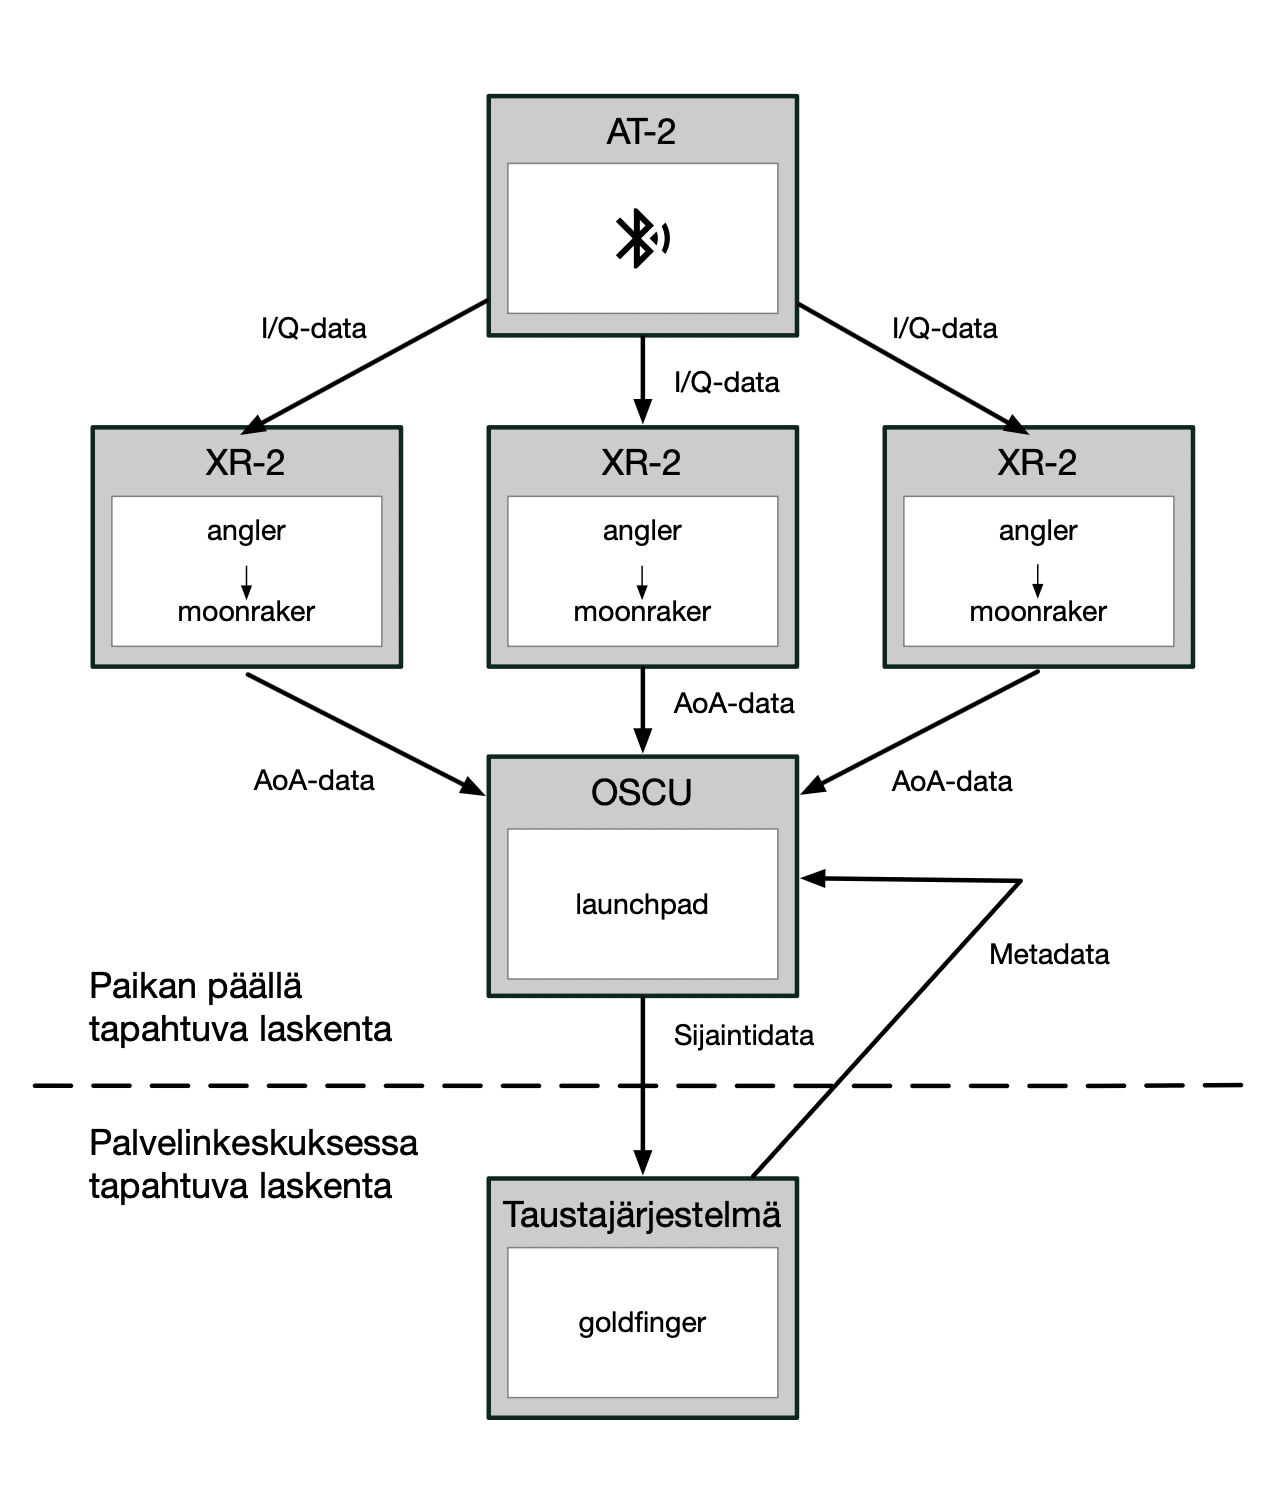
\includegraphics[width=15cm]{jarjestelmaarkkitehtuuri}
\caption{Järjestelmäarkkitehtuuri}
\label{fig:jarjestelmaarkkitehtuuri}
\end{figure}

Tässä luvussa keskitytään \emph{launchpad}-sovelluksen hyödyntämään paikannusalgoritmiin, mutta sitä ennen käsitellään lyhyesti tulokulman laskentamenetelmiä ja \emph{angler}-sovelluksen toimintaa. Immateriaalioikeussyistä tutkielmassa ei hyödynnetä Go-ohjelmointikielellä toteutettua ohjelmakoodia. Sen sijaan paikannusalgoritmi on toteutettu R-ohjelmointikielellä.

\subsection{AoA-menetelmistä} \label{aoa}

Riippuen käytetystä teknologiasta ja teknologian tuottamasta datasta, voidaan sisätilapaikannuksessa soveltaa lukuisia eri paikannustekniikkoja ja -algoritmeja. Oguntalaa (2018) \citep{oguntala-2018} mukailevassa kaaviossa \ref{fig:paikannusmenetelmat} on esitetty pääpiirteittäin sisätilapaikannusmenetelmät käytetyn datan (kaaviossa oikealla) mukaan jaoteltuna.

\begin{figure}[H]
\centering
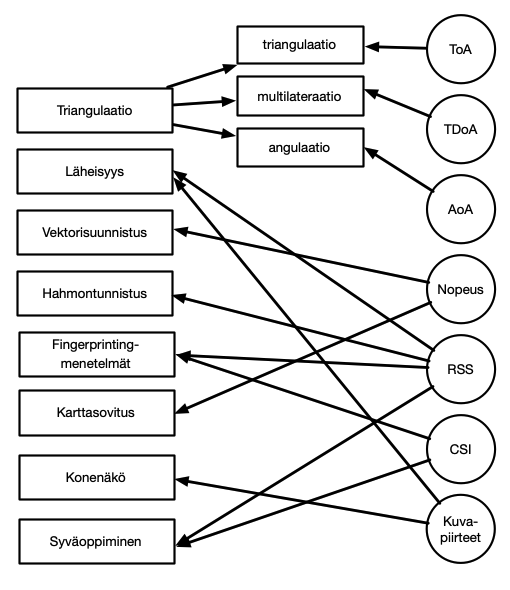
\includegraphics[width=12.5cm]{paikannusmenetelmat}
\caption{Paikannusmenetelmien luokittelu}
\label{fig:paikannusmenetelmat}
\end{figure}

Walkbasen toteuttama paikannusratkaisu perustuu AoA-menetelmään. Tämä on paikannusteknologia, joissa lähettimen ja vastaanottimen välinen kulma estimoidaan signaalin saapumiskulman perusteella. Tässä estimoinnissa hyödynnetään signaalin vaihe-eroja, kun sama signaali vastaanotetaan usealla eri antennilla.

Walkbase käyttää radiosignaalien tulokulman estimoinnissa MUSIC-algoritmia (\emph{Multiple Signal Classification}), joka arvioi tulokulmia analysoimalla signaalien autokorrelaatiomatriisia ja etsimällä sen ominaisvektoreita. Esitys MUSIC-algoritmista löytyy esimerkiksi Hayesin kirjasta \emph{Statistical Digital Signal Processing and Modeling} (1996) \citep{Hayes-1996}. Guniam \&al (2023) \citep{Gunia-2023} puolestaan esittävät artikkelissa ``Analysis and Design of a MuSiC-Based Angle of Arrival Positioning System'' tapoja optimoida MUSIC-algoritmia soveltumaan monimutkaisiin, heijastuksia sisältäviin sisätilaympäristöihin.

\emph{Angler}-sovellus hyödyntää MUSIC-algoritmin toteutuksessa omaa hiukkassuodinalgoritmiaan signaalispektrin analysointiin sekä tulokulmien estimointiin. MUSIC-algoritmia tai \emph{angler}-sovelluksen hiukkassuodinalgoritmia ei käsitellä tarkemmin tämän tutkielman puitteissa.

\subsection{Kalibraatiosta}

Koska \emph{angler}-sovellus laskee suuntimakulman aina antenniryhmän määrätystä reunasta nähden, on tärkeää, että laitteen asemointi karttapohjoiseen nähden on tiedossa. Koska laitteen tarkan kulman arvioiminen asennusympäristössä on haastavaa eikä laite sisällä kompassia, kalibroidaan kukin laite SIR-kalibraatioalgoritmilla, jonka on mahdollista ottaa huomioon myös laitteen IMU-intertiamittausyksiköstä saatavat kallistumis- ja nyökkäämiskulmat.

Jos IMU-dataa hyödynnetään, tuottaa kalibraatioalgoritmi jokaiselle XR-2-laitteelle rotaatiomatriisin \(\mathbf{R}_l\). Muussa tapauksessa kalibraatioalgoritmi tuottaa jokaiselle laitteelle atsimuuttiakulman kohdistuksen \(\eta\). Kalibraatioalgoritmia ei käsitellä tämän tutkielman puitteissa. Paikannusongelman yksinkertaistamiseksi myöskään IMU-yksikön tuottamaa dataa ei sisällytetä kalibraatioon ja jokaisen XR-2-laitteen oletetaan olevan lattiaan nähden vaakatasossa. Atsimuuttikulman kalibraatiokohdistuksesta lisää seuraavassa alaluvussa \ref{datan-kuvaus}.

\section{Datan kuvaus} \label{datan-kuvaus}

Koeasetelmaa varten AT-2-tagi on asetettu lähettämään I/Q-dataotoksia 6hz taajuudella, joka vastaa järjestelmän tuotantokäyttöä. Parempi sijaintitarkkuus saavutettaisiin korkeammalla taajuudella, mutta käytännön sovellutuksissa ei tagien akun kesto salli 6hz korkeampaa lähetystaajuutta.

\emph{Angler}-sovellus koostaa jokaisesta tagin lähettämästä dataotoksesta \(s\) atsimuutti- eli suuntimakulman \(\theta_s\) ja korkeuskulman \(\gamma_s\), jotka noudattavat suuntimakulman osalta von Mises -jakaumaa ja korkeuskulman osalta katkaistua normaalijakaumaa:

\begin{align}
&\theta_{s} \sim \text{von Mises}(\mu_{\theta_s}, \kappa_k),\\
&\gamma_{s} \sim \mathcal{N}_{\text{katkaistu}} (\mu_{\gamma_s}, \sigma^2_s).
\end{align}

Jakaumat on kuvattu tarkemmin alaluvussa \ref{uskottavuusmallit}. Jokaisen XR-2-laitteen \emph{angler}-sovellus lisää dataan myös sekvenssinumeron, jonka perusteella samasta AT-2-tagin lähettämästä I/Q-dataoksesta lasketut usean eri vastaanottimen laskemat tulokulmat voidaan yhdistää samaan I/Q-dataotokseen. XR-2-laitteen lähettämä tulokulmadata on kuvattu alla.

\def\arraystretch{1.25} 
\begin{table}[H]
\centering
\begin{tabular}{|l|l|l|}
\hline
Muuttuja & Kuvaus & Esimerkkiarvo\\
\hline
id & havainnon yksilöivä tunniste & 317092 \\
ts & havainnon aikaleima & \makecell[l]{2024-04-08 \\ 21:38:20.998+00}\\
locator\_mac & XR-2-laitteen MAC-osoite & 2c:e3:10:00:07:a6
\\
asset\_tag\_mac & AT-2-tagin MAC-osoite & 2c:e3:10:00:63:89\\
sequence\_nr & \makecell[l]{kulmadatan I/Q-dataotokseen yhdistävä \\ juokseva numerointi} & 2066\\
azimuth\_location & \makecell[l]{atsimuuttikulman $\theta$ \\ jaukauman sijaintiparametri $\mu_{\theta}$ (rad)} & 0.39
\\
azimuth\_scale & \makecell[l]{atsimuuttikulman $\theta$ \\ jaukauman skaalaparametri $\kappa$} & 80.98
\\
elevation\_location & \makecell[l]{korkeuskulman $\gamma$ \\ jaukauman sijaintiparametri $\mu_{\gamma}$ (rad)} & 0.13
\\
elevation\_scale & \makecell[l]{korkeuskulman $\gamma$ \\ jaukauman skaalaparametri $\sigma^2$} & 0.012
\\
quality\_sndr & signaali-kohinasuhde & 22.0 \\
rssi & signaalin vahvuus (dBm) & -81\\
distance & arvioitu etäisyys lähettimeen (m) & 18.6\\
\hline
\end{tabular}
\caption{Tulokulmamuuttujat}
\label{tab:aoa-muuttujat}
\end{table}

Etäisyys on estimoitu signaalin vahvuudesta käyttäen propagaatiomallia. Etäisyyttä tai signaalin vahvuutta ei käytetä paikantamiseen, joten tämän mallin käsittely jätetään tutkielman ulkopuolelle. Munoz (2009) luku 2 sisältää yleiskatsauksen propagaatiomalleista \citep{Munoz-2009}.

\emph{Launchpad}-sovelluksessa tulokulmadataan yhdistetään XR-2-laitteen MAC-osoitteen perusteella tarvittavat XR-2-laitteita koskevat metadatamuuttujat. Näihin kuuluvat laitteen korkeus, laitteen suuntimakulma ja karttakoordinaatit. Metadata on kuvattu taulukossa \ref{tab:metadata}.

\def\arraystretch{1.25} 
\begin{table}[H]
\centering
\begin{tabular}{|l|l|l|}
\hline
Muuttuja & Kuvaus & Esimerkkiarvo\\
\hline
locator\_mac & XR-2-laitteen MAC-osoite & b8:27:eb:66:0d:2a\\
lat & vastaanottimen sijainti (leveyspiiri) & 60.448265\\
lon & vastaanottimen sijainti (pituuspiirit) & 22.294823\\
direction & suuntimakulma $\eta$ (astetta) & 34\\
height & vastaanottimen korkeus (m) & 2.22 \\
\hline
\end{tabular}
\caption{Metadata}
\label{tab:metadata}
\end{table}

Atsimuuttikulma \(\theta\) lasketaan aina vastaanottimen tietyltä sivulta, joten se vastaa napapohjoista ainoastaan siinä tapauksessa, että vastaanottimen kyseinen sivu on asetettu kohtisuoraan napapohjoiseen nähden. Käytännössä vastaanottimien asettaminen tiettyyn kulmaan ei ole aina mahdollista eikä vaihe-erojen mittaamisen kannalta edes suotavaa. Tämän vuoksi jokaiselle vastaanottimelle on tietokantaan tallennettu oma suuntimakulma \(\eta\). Toisin kuin tulokulmadatan kulmat, on tämä tallennettu tietokantaan asteina. Kokeessa käytetään napapohjoisesta laskettuja kulmia \(\Phi\), jotka lasketaan jokaiselle havainnolle havainnon vastaanottimen suuntimakulman avulla

\begin{align}
\Phi=(\theta + \eta \times \frac{\pi}{180^\degree}) \mod 2 \pi.
\end{align}

Lisäksi saatavilla on PostGIS-muotoon tallennettua polygonidataa, joka kuvaa koeympäristön pohjapiirrustusta sekä koeympäristössä esiintyviä liikkumisen estäviä kohteita, kuten hyllyjä tai pöytiä. Näitä hyödynnetään alaluvun \ref{karttasovitusalgoritmi} karttasovitusalgoritmissa.

Havaintomuuttujien ohella koetilanteesta on tallennettu testipolku, jota pitkin AT-2-tagia liikutetaan koetilanteessa. Testipolkudata pitää sisällään karttaan piirretyn janan pääte- ja sisäpisteet. Tallennettu sijainti perustuu koeympäristön lattiaan pohjapiirrustusten sekä laser-mittausten avulla tehtyihin merkintöihin. Näin saadut testimuuttujat on kuvattu taulukossa (\ref{tab:testimuuttujat}).

\def\arraystretch{1.25} 
\begin{table}[H]
\centering
\begin{tabular}{|l|l|l|}
\hline
Muuttuja & Kuvaus & Esimerkkiarvo\\
\hline
path\_lat & polkupisteen sijainti (leveyspiiri) & 60.44819 \\
path\_lon & polkupisteen sijainti (pituuspiiri) & 22.29493 \\
\hline
\end{tabular}
\caption{Testimuuttujat}
\label{tab:testimuuttujat}
\end{table}

\noindent Alaluvussa \ref{karttasovitusalgoritmi} kuvatulla interpolaatiolla metreiksi muutettuja testimuuttujia käytetään paikannusalgoritmien paikannusvirheen laskemisessa. Koska koeasetelmassa (kts. alaluku \ref{koeasetelma}) ei laitteen sijaintia tallenneta dataa kerättäessä, käytetään paikannusvirhettä laskettaessa janojen päätepisteiden joukosta tiivistettyä joukkoa. Paikannusvirheen laskenta on kuvattu algoritmissa \ref{testipolun-tihennys}.

\begin{algorithm}[H]
\label{testipolun-tihennys}
\DontPrintSemicolon
\SetAlgoShortEnd
\KwResult{Aika-askeleen $k$ paikannusvirhe $\epsilon_{\text{pos}_k}$ (m);}
\KwData{Metreiksi muutetut testimuuttujat sisältävä pistejoukko $P$. Aika-askeleen $k$ sijaintiestimaatti $\hat{x}_k$. Tihennysparametri $s$, vakioarvo $s=1000$.\;}
\Begin{
  \Begin{Tihennetään pistejoukko $P$. Lisätään joukosta $P$ luoduille janoille pisteitä lineaarisella interpolaatiolla, kunnes joukossa on $s$ pistettä. Saadaan joukko $S$.;}
  \Begin{Asetetaan $\hat{\epsilon}_{\text{pos}_k}= \infty$;}
  \For{$i=\{1,2,\ldots,s\}$}{
      \Begin{Lasketaan sijaintiestimaatin $\hat{x}_k$ ja pisteen $S_i$ välinen Euklidinen etäisyys $d_i$.\;}
      \If{$d_i < \hat{\epsilon}_{\text{pos}_k}$}{\Begin{$\hat{\epsilon}_{\text{pos}_k}=d_i$;}}
    }
  \Begin{Palautetaan aika-askeleen $k$ paikannusvirhe $\epsilon_{\text{pos}_k}=\hat{\epsilon}_{\text{pos}_k}$;}
  }  
\caption{Paikannusvirheen laskeminen}
\end{algorithm}

\noindent Algoritmiin palataan alaluvun \ref{empiirinen-esimerkki} empiirisessä esimerkissä.

\subsection{Karttaprojektioista} \label{karttaprojektioista}

Kaikki yllä esitetyssä datassa esiintyvät sijaintikoordinaatit on tallennettu tietokantaan WGS 84 -tasokoordinaattijärjestelmässä. Hiukkassuotimiin perustuvaa paikannusalgoritmia sovellettaessa on kuitenkin monin paikoin tarve syöttää parametreja metrijärjestelmässä. Tästä syystä leveys- ja pituusasteisiin perustuvat koordinaatit muunnetaan laskentaa varten metreiksi ja metreinä esitetyt sijaintitulokset muutetaan tulosten esittämistä varten takaisin WGS 84 -koordinaattijärjestelmään.

Muunnos tapahtuu lineaarisella interpolaatiolla. Määritellään ensin kerrospolygonin rajausalue. Koska kaikki käytetyt koordinaatit ovat tämän rajausalueen sisällä, voidaan tätä rajausaluetta käyttää metrikonversiossa. Rajausalue koostuu neljästä kulmapisteestä. Poimitaan näistä pisteistä minimit ja maksimit sekä pituus- että leveyskoordinaateille. Näin saadaan neljä arvoa \(B_{\text{lonlat}}=\{\text{lon}_{\text{min}}, \text{lon}_{\text{max}}, \text{lat}_{\text{min}}, \text{lat}_{\text{max}}\}\). Määritellään rajausalueen sivujen pituus metreinä geodeettisen etäisyyden avulla, jolloin saadaan kaksi metreissä laskettua etäisyyttä \(D_{\text{m}}=\{d_{\text{lon}}, d_{\text{lat}}\}\). Käytetään näitä kulmapisteitä sekä metreinä laskettuja etäisyyksiä interpoloimaan koordinaatit WGS 84 -koordinaattijärjestelmästä metreissä esitetyille arvoalueille \([0, \text{max}(x_m)]\) ja \([0, \text{max}(y_m)]\) seuraavasti:

\begin{align}\label{wgs84-m}
x_m = f(x_{\text{lon}}; B_{\text{lonlat}}, D_m) = \frac{x_{\text{lon}} -\text{lon}_{\text{min}}}{\text{lon}_{\text{max}}-\text{lon}_{\text{min}}} \times d_{\text{lon}},\\
y_m = f(y_{\text{lat}}; B_{\text{lonlat}}, D_m) = \frac{y_{\text{lat}} -\text{lat}_{\text{min}}}{\text{lat}_{\text{max}}-\text{lat}_{\text{min}}} \times d_{\text{lat}}
,\end{align}

\noindent missä \(x_m\) vastaa leveyskoordinaatteja metreissä ja \(y_m\) pituuskoordinaatteja metreissä. Vastaavasti käännös takaisin WGS 84 -koordinaattijärjestelmään tapahtuu seuraavasti:

\begin{align}\label{m-wgs84}
x_{\text{lon}} = f(x_m; B_{\text{lonlat}}, D_m) = \frac{x_{\text{m}}}{d_{\text{lon}}} \times (\text{lon}_{\text{max}}-\text{lon}_{\text{min}}) + \text{lon}_{\text{min}},\\
y_{\text{lat}} = f(y_m; B_{\text{lonlat}}, D_m) = \frac{y_{\text{m}}}{d_{\text{lat}}} \times (\text{lat}_{\text{max}}-\text{lat}_{\text{min}}) + \text{lat}_{\text{min}}
.\end{align}

\noindent Empiirisessä esimerkissä jätetään takaisinmuunnos tekemättä, jotta koeympäristön sijaintia ei voi paikallistaa sen koordinaattien perusteella.

\subsection{Muunnettu data} \label{muunnettu-data-luku}

Kun dataan on tehty yllä esitetyt konversiot ja metadata on liitetty jokaisen aika-askeleen \(k\) dataan, saadaan data lopulliseen, empiirisessä esimerkissä käytettävään muotoon, jossa jokaisen aika-askeleen \(k\) kohdalla on käytettävissä seuraava data:

\def\arraystretch{1.25} 
\begin{table}[H]
\centering
\begin{tabular}{|l|l|l|}
\hline
Muuttuja & Kuvaus & Esimerkkiarvo\\
\hline
id & havainnon yksilöivä tunniste & 317092 \\
ts & havainnon aikaleima & \makecell[l]{2024-04-08 \\ 21:38:20.998+00}\\
locator\_mac & XR-2-laitteen MAC-osoite & 2c:e3:10:00:07:a6
\\
asset\_tag\_mac & AT-2-tagin MAC-osoite & 2c:e3:10:00:63:89\\
sequence\_nr & \makecell[l]{kulmadatan I/Q-dataotokseen yhdistävä \\ juokseva numerointi} & 2066\\
azimuth\_location\_mdf & \makecell[l]{atsimuuttikulman $\theta$ \\ jaukauman muunnettu sijaintiparametri \\ $\Phi$ (rad)} & 0.39
\\
azimuth\_scale & \makecell[l]{atsimuuttikulman $\theta$ \\ jaukauman skaalaparametri $\kappa$} & 80.98
\\
elevation\_location & \makecell[l]{korkeuskulman $\gamma$ \\ jaukauman sijaintiparametri $\mu_{\gamma}$ (rad)} & 0.13
\\
elevation\_scale & \makecell[l]{korkeuskulman $\gamma$ \\ jaukauman skaalaparametri $\sigma^2$} & 0.012
\\
quality\_sndr & signaali-kohinasuhde & 22.0 \\
rssi & signaalin vahvuus (dBm) & -81\\
distance & arvioitu etäisyys lähettimeen (m) & 18.6\\
x\_m & \makecell[l]{vastaanottimen sijainti \\ ($x$-koordinaatti, metreinä)} & 1.24\\
y\_m & \makecell[l]{vastaanottimen sijainti \\ ($y$-koordinaatti, metreinä)} & 0.78\\
height & vastaanottimen korkeus (m) & 2.22 \\
\hline
\end{tabular}
\caption{Muunnettu data}
\label{tab:muunnettu-data}
\end{table}

\section{Sisätilapaikannusalgoritmi}

\subsection{Ongelman kuvaus} \label{ongelman-kuvaus}

Tarkoituksena on estimoida liikkuvan AT-2-tagin sijaintia. Merkitään estimoitavaa tilasarjaa \(x_{1:k}=\{x_1,\ldots,x_k\}\), missä sijainnit on estimoitu sekunnin tarkkuudella. Lisäksi merkitään \(x_0\) testilaitteen lähtösijaintia. Jokainen tilasarjan havainto koostuu suuntimakulmasta sekä pituus- että leveyskoordinaateista \((x_k^x, x_k^y)\). Määritellään tilalle liikkuvan AT-2-tagin kulkua kuvaava vektorisuunnistukseen (\emph{dead reckoning}) perustuva dynaaminen malli (\ref{tilamalli-liikkuva})

\begin{align}\label{tilamalli-liikkuva}
x_{k+1}=f(x_k, \nu_k)=x_k+D_k \begin{bmatrix} \cos\psi_k \\ \sin\psi_k \end{bmatrix}+\nu_k,
\end{align}

\noindent missä \(D_k\) on AT-2-tagin sekunnin aika-askeleen \(k \rightarrow k+1\) aikana kulkema matka ja \(\psi_k\) AT-2-tagin liikkeen suuntimakulma kyseisellä aika-askeleella. \(\nu_k\) on kohinaa, joka syntyy mittausvirheestä ja jolle voidaan olettaa \(\sim \mathcal{N}(\mu_x,\,\sigma_x^{2})\). Jos laite on paikallaan, yksinkertaistuu malli muotoon \(x_{k+1}=f(x_k)=\text{id}(x_k)=x_k\), missä \(\text{id}(x)\) on identiteettifunktio.

Vastaavasti \(y_{k_{i,j}}=\{y_{k_{1,1}},\ldots,y_{k_{n_s,z}}\}\) kuvaa AT-2-tagin ja XR-2-laitteiden välillä yhden sekuntin aika-askeleen aikana laskettuja kulmahavaintoja, missä \(i=1,\ldots,n_s\) käy läpi kaikki \(n_s\) XR-2-laitetta ja \(j=1,\ldots,z\) kustakin laitteesta vastaanotetut kulmahavainnot. \(z\) ilmaisee tässä AT-2-tagin lähetystaajuutta, joka koeasetelmassa on \(z=6\). Näin ollen jokainen havainto koostuu (maksimissaan) \(6\times n_s\) kappaleesta kulmahavaintoja.

Lisäksi tunnetaan XR-2-laitteisiin \(\{s^1,\ldots,s^{n_s}\}\) liittyvät leveys- ja pituuskoordinaatit \((\lambda, \phi)\), jotka on muutettu alaluvussa \ref{karttaprojektioista} esitetyllä interpolaatiolla metreiksi. Saadaan

\begin{align}
u=\begin{bmatrix} \lambda^1 & \phi^1 \\  \lambda^1 & \phi^1 \\  \vdots & \vdots \\ \lambda^{n_s} & \phi^{n_s} \end{bmatrix},
\end{align}

\noindent missä jokainen koordinaattipari on toistettu \(z\) kertaa. Määritellään nyt havaintomalli

\begin{align}\label{havaintomalli}
y_{k_{i,j}}=h(x_k, u)+e_k=\text{atan2} \left( \begin{bmatrix}\phi^1-x_k^y\\ \phi^1-x_k^y\\ \vdots \\ \phi^{n_s}-x_k^y\end{bmatrix}, \begin{bmatrix}\lambda^1-x_k^x\\ \lambda^1-x_k^x\\ \vdots \\ \lambda^{n_s}-x_k^x\end{bmatrix} \right) +e_k,
\end{align}

\noindent missä

\begin{align}\label{atan2}
\displaystyle \operatorname{atan2}(y,x)={\begin{cases}\arctan({\frac {y}{x}})&{\text{jos }}>0,\\\arctan({\frac {y}{x}})+\pi &{\text{jos }}<0{\text{ ja }}y\geq 0,\\\arctan({\frac {y}{x}})-\pi & {\text{jos }}>0{\text{ ja }}<0,\\+{\frac {\pi }{2}}&{\text{jos }}x=0{\text{ ja }}>0,\\-{\frac {\pi }{2}}&{\text{jos }}x=0{\text{ ja }}<0,\\{\text{ei määritelty}}&{\text{jos }}x=0{\text{ ja }}y=0\end{cases}}
\end{align}

\noindent ja kohina noudattaa moniulotteista normaalijakaumaa \(e_k\sim\mathcal{N}(0,{\Sigma})\).

Määrittelemätön \(\text{atan2}\)-tapaus, jossa \(x=0\) ja \(y=0\) on käytetyllä mittaustarkkuudella käytännössä mahdoton. Jos tapaus halutaan kuitenkin välttää, voidaan nolla-arvot tarpeen vaatiessa korvata joillakin hyvin lähellä nollaa olevalla arvolla.

Kumpikaan funktiosta \(h(\cdot)\) ja \(f(\cdot)\) ei ole lineaarinen, joten SIR-algoritmi on sopiva valinta ongelman ratkaisemiseksi. Koetuloksia arvioidaan ensisijaisesti paikannusvirheen avulla. Paikannusvirhe \(\epsilon_{\text{pos}_k}\) lasketaan jokaisen aika-askeleen \(k\) posteriorijakaumaestimaatista \(\hat{p}_k\) painotettuna keskiarvona

\begin{align}
\epsilon_{\text{pos}_k} = d\left( P_k, \sum_{i=1}^Nw^k_ix^i_k \right),
\end{align}

\noindent missä \(w_i^k\) on ajanketken \(k\) partikkelien normalisoitu paino ja \(d(x^i_k,y_k)\) partikkelien ja testilaitteen todellisen sijainnin \(P_k\) välisen etäisyyden algoritmilla \ref{testipolun-tihennys} laskeva funktio.

\hypertarget{uskottavuusmallit}{%
\subsection{Uskottavuusmallit}\label{uskottavuusmallit}}

Jokainen yhtä tulokulmaa vastaava \emph{angler}-sovelluksen tuottama havaintodatarivi pitää sisällään neljä parametrimuuttujaa \texttt{azimuth\_location\_mdf}, \texttt{azimuth\_scale}, \texttt{elevation\_location} ja \texttt{elevation\_scale}. Koska \emph{angler}-sovellus on kirjoitettu varta vasten tuottamaan dataa hiukkassuodinpaikannusalgoritmia varten, ovat nämä valmiiksi hiukkassuotimen uskottavuusmallin parametreja.

\emph{Angler}-sovelluksessa XR-2-laitteen ja AT-2-tagin välinen atsimuuttikulma simuloidaan von Mises -jakaumasta, jolloin muuttujat \texttt{azimuth\_location\_mdf} ja \texttt{azimuth\_scale} vastaavat tämän jakauman sijainti- ja skaalaparametreja \(\mu\) ja \(\kappa\). Näistä edellistä voidaan pitää itse atsimuuttikulman estimaattina. Määritellään siis jokaiselle tulokulmalle \(h\) sekä XR-2-laitteelle \(l\) seuraava atsimuuttikulman uskottavuusmalli:

\begin{align}\label{atsimuutti-uskottavuusmalli}
L_{\theta_{h,l}}(y_{h,l}|x_{h,l}; \mu_{h,l}, \kappa_{h,l})=\frac{e^{\kappa_{h,l} \text{cos}(x_{h,l}-\mu_{h,l})}}{2 \pi I_0(\kappa_{h,l})},
\end{align}

\noindent missä \(I_0\) on 0:s ensimmäisen lajin Bessel-funktio ja \(x_{h,l}\) on jokaisen hiukkasen \(n=1,\ldots,N\) sekä XR-2-laitteen \(l\) välinen suuntimakulma.

Vastaavasti \emph{angler}-sovelluksessa XR-2-laitteen ja AT-2-tagin välinen korkeuskulma simuloidaan katkaistusta normaalijakaumasta, jolle \(a=0\) ja \(b=\pi/2\). Nyt muuttujat \texttt{elevation\_location} ja \texttt{elevation\_scale} vastaavat tämän jakauman sijainti- ja skaalaparametreja \(\mu\) ja \(\sigma^2\) ja näistä edellistä voidaan pitää itse korkeuskulman estimaattina. Määritellään jokaiselle tulokulmalle \(h\) sekä XR-2-laitteelle \(l\) seuraava korkeuskulman uskottavuusmalli:

\begin{align}\label{korkeus-uskottavuusmalli}
L_{\gamma_{h,l}}(y_{h,l}|x_{h,l}; \mu_{h,l}, \sigma^2_{h,l}, a=0, b=\pi/2)=\frac{1}{\sqrt{2 \pi}} \text{exp}\left(-\frac{(x_{h,l}-\mu_{h,l})}{2 \sigma^2}\right) / \sqrt{\sigma^2}Z_{h,l},
\end{align}

\noindent missä \(Z_{h,l}=\frac{1}{2}(1+\text{erf}(\frac{b-\mu_{h,l}}{\sqrt{\sigma^2}}))-\frac{1}{2}(1+\text{erf}(\frac{a-\mu_{h,l}}{\sqrt{\sigma^2}}))\) ja \(x_{h,l}\) on jokaisen hiukkasen \(n=1,\ldots,N\) sekä XR-2-laitteen \(l\) välinen korkeuskulma.

Uskottavuusmallit (\ref{atsimuutti-uskottavuusmalli}) ja (\ref{korkeus-uskottavuusmalli}) kertomalla saadaan yhdistetty uskottavuusmalli hiukkassuotimen aika-askeleelle \(k\) sekä XR-2-laitteelle \(l\)

\begin{align}\label{yhdistetty-uskottavuusmalli}
L_{k,l}=\prod_{h=1}^{z} L_{\theta_{h,l}} \times \prod_{h=1}^{z} L_{\gamma_{h,l}},
\end{align}

\noindent josta voidaan edelleen laskea jokaisen hiukkasen uskottavuus aika-askeleella \(k\) kertomalla XR-2-laitteita vastaavat uskottavuudet keskenään

\begin{align}\label{lopullinen-uskottavuusmalli}
L_{k}=\prod_l^{n_s} L_{{k,l}}.
\end{align}

Koska yllä esitettyjen mallien uskottavuudet ovat käytännössä erittäin pieniä, käytetään numeerisista syistä itse algoritmissa logaritmoituja uskottavuusmalleja, jolloin \(l_{k,l} = \sum\text{log}(L_{\theta_{k_l}}) + \sum\text{log}(L_{\gamma_{k_l}})\) ja \(l_k = \sum_l^{n_s} l_{k,l}\).

\hypertarget{datan-valinta}{%
\subsection{Datan valinta}\label{datan-valinta}}

Koska Walkbasen paikannusjärjestelmä toimii monimutkaisessa, heijastuksia sisältävässä radioympäristössä, suoritetaan jokaisella aika-askeleella \(k\) vielä ylimääräinen datan valinta. Valinnan tarkoituksena on jättää mahdollisia heijastuksia sisältävät tai muuten selkeästi virheelliset tulokulmat paikannusdatan ulkopuolelle.

Yksinkertaisin tapa valita käytettävät kulmat on asettaa alaraja signaalin vahvuudelle, jolloin ainoastaan tiettyä kynnys-dBm-arvoa suuremman signaalin vahvuuden omaavat tulokulmat valitaan paikannukseen. Datan valinta suoritetaan kunkin aika-askeleen alussa ja tyypillisiä kynnysarvoja ovat esimerkiksi \(-100\)dBm, \(-90\)dBm ja \(-80\)dBm. Jos kynnysarvo ei ole käytössä, käytetään ohjelmakoodissa arvoa \(-120\)dBm, joka jättää kaikki tulokulmat dataan. Datan valintaan palataan parametrien valinnan yhteydessä alaluvussa \ref{parametrien-valinta}.

\hypertarget{dynaaminen-malli}{%
\subsection{Dynaaminen malli}\label{dynaaminen-malli}}

Dynaamisen mallin tehtävänä on liikuttaa hiukkasia aika-askeleiden \(k\) ja \(k+1\) välillä. Dynaaminen malli perustuu vektorisuunnistusmalliin (\ref{tilamalli-liikkuva}). Vastaavaa mallia hyödyntää muun muassa Solin (2016) \citep{Solin-2016}. Koska AT-2-tagi ei kuitenkaan lähetä nopeus- tai suuntadataa, asetetaan vektorisuunnistusmallin nopeutta ilmaiseva skalaarimuuttuja \(D_k=0\), jolloin malli yksinkertaistuu satunnaiskävelymalliksi

\begin{align}\label{dynaaminen-malli-empiirinen}
x_{k+1}=x_k + v_k,
\end{align}

\noindent missä \(v_k\) on kohinaa. Kohina luodaan jokaiselle aika-askeleelle seuraavasti. Ensin luodaan etäisyysvektori \(d_k\) katkaistusta normaalijakaumasta, jonka sijaintiparametri on 0, katkaisukohdat \(a=0\) ja \(b=10\) ja jonka keskihajonta \(q\) on paikannusalgoritmin suunnitteluparametri:

\begin{align}
&d_k \sim \mathcal{N_{\text{katkaistu}}}(\mu=0, \sigma=q, a=0, b=10).
\end{align}

Tämän jälkeen luodaan suuntavektori \(p\) tasajakaumasta

\begin{align}
&p_k\sim\mathcal{U}(0, 2 \pi)
\end{align}

\noindent ja lopulta kohinavektori

\begin{align}
&v_k = (\text{cos}(p_k) \times d_k, \text{sin}(p_k) \times d_k),
\end{align}

\noindent missä vektorin ensimmäinen elementti vastaa sijaintien leveysasteiden kohinaa ja toinen elementti pituusasteiden kohinaa.

\hypertarget{paikallaanolon-havaitseminen}{%
\subsubsection{Paikallaanolon havaitseminen}\label{paikallaanolon-havaitseminen}}

Virransäästyösyistä AT-2-tagi lähettää dataa ainoastaan liikkuessaan. Jos laite ei ole 10 sekunnin aikana havainnut IMU-yksikkönsä perusteella kiihtyvyyttä, lopettaa laite datan lähettämisen. Laite on tällöin valmiusmoodissa. Tätä tietoa voidaan hyödyntää vaimentamalla dynaamisen mallin kohinaa, kun laitteen tiedetään olevan paikallaan. Jos paikannusalgoritmiin lisätään tarvittava 10 sekunnin viive, voidaan tätä viivettä hyödyntää paikallaanolon tehokkaampaan havaitsemiseen.

Jos yksikään XR-2-laite ei ole havainnut tagia aika-askeleen \(k\) aikana, voimme olettaa laitteen olevan valmiusmoodissa ja siten myös paikoillaan. Huomattavaa on kuitenkin, ettei päinvastainen päde. Paikoillaan oleva laite ei välttämättä ole valmisumoodissa, sillä valmiusmoodiin siirtyminen kestää 10 sekuntia. Tähän tietoon perustuen voidaan havaita paikallaanolo jo ennen kuin laite lopettaa datan lähettämisen ja vaimentaa dynaamista mallia algoritmin \ref{paikallaanoloalgo} avulla. Algoritmi ajetaan jokaisella aika-askeleella \(k\) ennen hiukkasten siirtoa dynaamisen mallin avulla.

\begin{algorithm}[H]
\label{paikallaanoloalgo}
\DontPrintSemicolon
\SetAlgoShortEnd
\KwResult{Positiivinen kokonaislukumuuttuja $m$, joka osoittaa kuinka moneksi aika-askeleeksi dynaamista mallia tulee vaimentaa. Jos $m=0$ mallia ei vaimenneta.;}
\KwData{Tagin tulokulmadata $L+1$ aika-askeleelle (nykyinen aika-askel + $L$ aika-askelta tulevaisuuteen). $L$ tulee asettaa niin, että paikallaan oleva tagi ehtii valmiustilaan. Jos saatavilla, edellinen muuttujan $m$ arvo. Algoritmin ensimmäisellä ajokerralla asetetaan $m=0$;}
\Begin{
  \Begin{Jos $m>0$, asetetaan $m=f(m)=m-1$ ja pysäytetään algoritmi. Jos $m=0$ jatketaan algoritmin suorittamista.;}
  \For{$l=\{k+1,\ldots,k+L\}$}{
    \Begin{Merkitään $o_l$ kulmahavaintojen määrää aika-askeleella $l$;}
    \If{$o_l = 0$ ja $m=0$}{\Begin{Asetetaan $m=l-k$;}}
    \Else{
      \If{$o_l=0$, $m>0$ ja $m+1=l-k$}{\Begin{Asetetaan $m=l-k$;}}}
  }  
}
\caption{Paikallaanolon havaitsemisalgoritmi}
\end{algorithm}

Yllä esitetty algoritmi etsii ensin ensimmäisen aika-askeleen, jonka aikana ei ole tallennettu lainkaan kulmahavaintoja ja asettaa muuttujan \(m\) arvon vastaamaan tätä aika-askelta. Jos algoritmi löytää useita peräkkäisiä aika-askeleita, joiden aikana ei ole tallennettu lainkaan kulmahavaintoija, valitsee se näistä suurimman. Koska koeasetelmassa AT-2-laitteen valmiustila aktivoituu 10 sekunnin kohdalla, valitaan \(L=10\).

Jos paikallaanolon havaitsemisalgoritmin nojalla dynaamista mallia päädytään vaimentamaan (so. \(m>0\)), asetetaan dynaamisen mallin keskihajonta-arvo \(q_{k}=\frac{q}{10}\). Dynaamista mallia ei siis täysin poisteta käytöstä, jotta paikannusalgoritmi pystyy tehokkaammin hyödyntämään myös vaimennettujen aika-askeleiden dataa. Näin sijaintiestimaatti konvergoi mahdollisimman lähelle todellista sijaintia, johon tagi on pysähtynyt.

\hypertarget{karttasovitusalgoritmi}{%
\subsubsection{Karttasovitusalgoritmi}\label{karttasovitusalgoritmi}}

Dynaamista mallia sovellettaessa voimme myös höydyntää saatavilla olevaa sisätilan karttadataa. Määritellään kaksi polygonityyppiä, lattiapolygoni \(F\) sekä estepolygonit \(E=\{E_1,\ldots,E_n\}\). Lattiapolygoni määrittää alueen, jonka sisällä hiukkassuodinalgoritmien hiukkasten pitää pysyä. Vastaavasti estepolygonien joukko määrittää lattiapolygonin sisällä alueet, joiden sisälle hiukkassuodinalgoritmin hiukkaset eivät voi siirtyä ja joiden läpi tagi ei voi kulkea. Käytännössä estepolygonit kuvaavat tilan seiniä sekä tiedossa olevia esteitä, kuten hyllyjä ja pöytiä.

Tarkastellaan ensin jokaisen \(i=1,\ldots,N\) hiukkasen kohdalla, siirtääkö dynaaminen malli hiukkasen polygonin \(F\) ulkopuolelle tai jonkin polygoneista \(E\) sisäpuolelle ja asetetaan näitä hiukkasia vastaavat painot nollaan.

\begin{align}\label{inclusion-polygon}
\displaystyle w^i_{k+1}={\begin{cases}w^i_{k+1}&\text{jos } x^i_{k+1} \in F,\\
0& \text{jos } x^i_{k+1} \notin F \lor x^i_{k+1} \in E \end{cases}}\end{align}

Tämän jälkeen tarkastellaan jokaisen jäljellä olevan (\(w^i_{k+1} \neq 0\)) mallin siirtämän hiukkasen polkua \(x_{k+1}^i-x_{k}^i\). Jos tämä polku ylittää yhden tai useamman estepolygonin \(E\) asetetaan kyseiselle hiukkaselle rangaistus seuraavasti:

\begin{align}\label{exclusion-polygon}
\displaystyle w^i_{k+1}={\begin{cases} \frac{1}{P} \times w^i_{k+1}&\text{jos } x^i_{k+1} \text{ ylittää estepolygonin},\\
w^i_{k+1}& \text{muulloin }\end{cases}}\end{align}

Tässä rangaistus \(P\) on algoritmin suunnitteluparametri. Vastaavaa toteutusta ovat hyödyntäneet muun muassa Davidson \&al (2010) \citep{Davidson-2010}, jotka ehdottavat rangaistusarvoa \(P=\frac{1}{1000}\). Rangaistuksen valintaan palataan parametrien valinnan yhteydessä alaluvussa \ref{parametrien-valinta}.

Koska erityisesti (\ref{inclusion-polygon}) asettaa hiukkasten painoja nollaan, eivät karttasovitetut hiukkaset välttämättä enää estimoi suodinjakaumaa tehokkaasti. Bojja \&al. \citep{Bojja-2015} ehdottavat suoritettavaksi uudelleenotantaa karttasovituksen jälkeen. Haluttaessa uudellenotanta suoritetaan seuraavasti. Merkitään nollapainoisten hiukkasten lukumäärää \(N_0\). Nyt otetaan uudet \(N_0\) otosta palauttaen joukosta \(\{x_{1:k}^i\}_{i=1}^N\), missä otoksen \(i\) todennäköisyys on \(w^i_{k|k}\). Korvataan nollapainoiset hiukkaset näin saadulla otoksella. Uudelleenotantaa ei käytetä empiirisessä esimerkissä, sillä se lisää tarvittavaa laskentatehoa ja hankaloittaa varianssin estimointia.

\subsection{Siloittelumalli} \label{siloittelumalli}

Koska haluttu sisätilapaikannusalgoritmi on online-algoritmi ja käytössä olevat laskennalliset resurssit ovat rajallisia, käytetään siloitteluun algoritmissa \ref{prediktiivinen-siloitin} esitettyä prediktiivistä siloitinta. Alaluvussa \ref{empiirinen-esimerkki} esitettävässä empiirisessä esimerkissä on tästä huolimatta kaikki data algoritmin saatavilla, joten viivettä ei tarvitse lisätä itse algoritmiin. Siloittelu saavutetaan yksinkertaisesti päivittämällä aika-askeleella \(k < T\) painot seuraavan lauseen mukaan

\begin{align}
&w_k = w_k^i \bar{w}^i_{k+1}, \hspace{0.5cm} \text{missä } \bar{w}^i_{k+1} = \frac{\sum_{j=1}^{N}w_{k}^j p(x_{k+1}^i|x_k^j)}{q(x_{k+1}^i|x_k^i,y_{k+1})}
.\end{align}

Partikkelien siirtämiseen käytetty satunnaiskulkumalli ei ole siloittelualgoritmien kannalta optimaalinen, joten empiirisessä esimerkissä alla hyödynnetään koetarkoituksessa vain tätä yksinkertaista siloittelumallia.

\subsection{WB-sisätilapaikannusalgoritmi}

Alla esitetään luvun 3 SIR-algoritmiin (\ref{sir}) sekä aiemmin tässä luvussa esitettyihin algoritmeihin perustuva WB-sisätilapaikannusalgoritmi kokonaisuudessaan. Luettavuuden parantamiseksi algoritmi on jaettu kahteen osaan niin, että algoritmin runko kuvataan algoritmissa \ref{wb-positioning} ja sijaintiestimaatin luominen algoritmissa \ref{wb-positioning2}.

Algoritmin priorijakaumana \(p_{x_0}\) käytetään kahta toisistaan riippumatonta otosta tasajakaumista, joista toinen vastaa leveys- ja toinen pituusasteita. Jakaumien alkupisteet valitaan niin, että ne vastaavat pienimpiä paikantimien leveys- ja pituusasteista. Vastaavasti päätepisteet valitaan niin, että ne vastaavat suurimpia paikantimien leveys- ja pituusasteita.

\begin{align} \label{priorijakauma}
&p_{x_{0_{\text{lat}}}}\sim\mathcal{U}(\min{\lambda},\max{\lambda}),\\
&p_{x_{0_{\text{lon}}}}\sim\mathcal{U}(\min{\phi},\max{\phi}).
\end{align}

\noindent Koska järjestelmän on tarkoitus toimia ainoastaan paikantimien muodostaman suorakaiteen sisäpuolella, ovat valitut jakaumien päätepisteet riittävät. Kummastakin jakaumasta tehdään \(\sqrt{N}\) otosta, jolloin \(N\) partikkelia \(x^i_0\) saadaan näiden otosten permutaatioina. Alaluvussa \ref{uudelleenotantamenetelman-valinta} määritellyn signaali-kohinasuhteen (\ref{SNR}) voi todeta olevan hyvin matala, sillä koe-esimerkin dynaaminen malli (\ref{dynaaminen-malli-empiirinen}) noudattaa satunnaiskulkua ja on siten pelkkää kohinaa. Tämän perusteella WB-sisätilapaikannusalgoritmi käyttää ehdotusjakaumanaan tilavektorin ehdollista prioria \(p(x_k|x_{k-1})\). Hiukkasten määrän \(N\) sekä muiden suunnitteluparametrien valinnasta kts. alaluku \ref{parametrien-valinta} alla.

Koska esitetty priorijakauma \(p_{x_0}\) on epäinformatiivinen ja monimutkainen koeympäristö aiheuttaa monin paikoin heijastuksia, on mahdollista, että ensimmäisten aika-askeleiden aikana algoritmi tuottaa huonoja sijaintiestimaatteja. Tästä syystä algoritmia ajettaessa suoritetaan ensimmäisellä \(b=3\) aika-askeleella sisäänajo, jonka aikana karttasovitusta ei käytetä ja jonka aikana kohina-arvona käytetään arvoa \(q_{k}=q\times10\). Myöskään sijaintiestimaatteja ei sisäänajoaika-askeleilla luoda. Sisäänajon jälkeen sijaintiestimaatit \(\hat{x}_{1:b}\) korvataan ensimmäisellä sisäänajon jälkeisellä sijaintiestimaatilla \(\hat{x}_{b+1}\).

Algoritmin tuottamien estimaattien varianssi estimoidaan käyttäen ALVar-varianssiestimaattia. Käytännössä tämä tarkoittaa varianssin estimointia käyttäen OD-varianssiestimaattia (\ref{OD-varianssi}) niin, että viiveparametri \(\lambda\) valitaan mukautuvasti käyttäen yhtälöä (\ref{ALVar-lambda}). Koska empiirisessä esimerkissä estimoitavia ulottuvuuksia on kaksi, leveys- ja pituuskoordinaatit, lasketaan varianssi kummallekin näistä erikseen. Saadaan pituuskoordinaattien varianssiestimaatti \(\hat{\sigma}^2_{k_x}\) ja leveyskoordinaattien varianssiestimaatti \(\hat{\sigma}^2_{k_y}\).

Lasketaan lisäksi kovarianssiestimaatti

\begin{align}\label{ALVar-kovarianssi}
\hat{\text{Cov}}_k = \frac{1}{N-1} \sum_{i=1}^N w_k^i (x_{k_{x}}^i[E_{k(\lambda)}]-\hat{\mu}_{k_x})(x_{k_y}^i[E_{k(\lambda)}]-\hat{\mu}_{k_y})
,\end{align}

\noindent missä \(\hat{\mu}_{k_x}\) on painotettu summa (\ref{OD-sum}) laskettuna pituuskoordinaateille ja \(\hat{\mu}_{k_y}\) painotettu summa (\ref{OD-sum}) laskettuna leveyskoordinaateille. Viiveparametri \(\lambda\) on edelleen valittu mukautuvasti käyttäen yhtälöä (\ref{ALVar-lambda}). Yhdistetään estimoidut varianssit ja kovarianssi kovarianssimatriisin estimaatiksi

\begin{align}\label{ALVar-kovarianssimatriisi}
\hat{\mathbf{\Sigma}}_k = \begin{bmatrix} \hat{\sigma}^2_{k_x} & \hat{\text{Cov}}_k \\ \hat{\text{Cov}}_k & \hat{\sigma}^2_{k_y} \end{bmatrix}
\end{align}

\noindent ja lasketaan aika-askeleen \(k\) varianssiestimaatti kovarianssimatriisin Frobeniuksen normina

\begin{align}\label{WB-varianssi}
\hat{\sigma}_k = \norm{ \hat{\mathbf{\Sigma}}_k } = \sqrt{ \text{tr}\left(\hat{\mathbf{\Sigma}}_k * \hat{\mathbf{\Sigma}}_k\right)}
,\end{align}

\noindent jolloin saadaan jokaiselle aika-askeleelle yksi skalaariarvoinen varianssiestimaatti.

\afterpage{ 
\clearpage
\begin{algorithm}[H]
\label{wb-positioning}
\DontPrintSemicolon
\SetAlgoShortEnd
\KwResult{Tagin sijaintiestimaatti $\hat{x}$ kullekin aika-askeleelle $k=1,\ldots,T$, näitä vastaavat varianssiestimaatit $\hat{\sigma}_k^2$.;}
\KwData{Taulukossa \ref{tab:muunnettu-data} esitetty data $y_k$ kullekin aika-askeleelle $k=1,\ldots,T$\, alaluvussa \ref{karttasovitusalgoritmi} esitetty polygonimetadata. Taulukossa \ref{tab:wb-parametrit} esitetyt parametrit.;}
\Begin{
  \Begin{Luodaan priorijakauma $p_{x_0}$ otantana jakaumista (\ref{priorijakauma}), asetetaan painot $w_0=1/N$.;}
  \For{$k=\{1,\ldots,T\}$}{
    \If{$k > b$}{
    \Begin{Ajetaan paikallaanolon havaitsemisalgoritmi \ref{paikallaanoloalgo}. Jos havaitaan paikallaanolo, päivitetään kohina-arvo $q_k=\frac{q}{10}$, muussa tapauksessa $q_k=q$;}
    \Begin{Sovitetaan partikkeleihin dynaaminen malli (\ref{dynaaminen-malli-empiirinen}) $x_{k+1}=x_k + v_k$, missä $v_k$ on luotu alaluvussa \ref{dynaaminen-malli} esitetyllä menetelmällä sekä kohina-arvolla $q_k$;}
    } \Else{ \Begin {Sovitetaan partikkeleihin dynaaminen malli (\ref{dynaaminen-malli-empiirinen}) $x_{k+1}=x_k + v_k$, missä $v_k$ on luotu alaluvussa \ref{dynaaminen-malli} esitetyllä menetelmällä sekä kohina-arvolla $q_k=q\times10$;}}
    \Begin{Jos karttasovitusalgoritmi on käytössä ja $k>b$, päivitetään painot $w_k$ alaluvun \ref{karttasovitusalgoritmi} karttasovitusalgoritmilla ja rangaistusarvolla $P$;}
    \Begin{Päivitetään painot ja luodaan sijaintiestimaatti algoritmilla \ref{wb-positioning2};}
    \Begin{Lasketaan ALVar-varianssi $\hat{\sigma}^2_k$.\;}
    \Begin{Lasketaan efektiivinen otoskoko $\hat{N}_{eff}$.\;}
    \If{$\hat{N}_{eff}< N_{th}$}{\Begin{Otetaan uudet $N$ otosta palauttaen joukosta $\{x_{1:k}^i\}_{i=1}^N$, missä otoksen $i$ todennäköisyys on $w^i_{k|k}$.\;}}
    \Begin{Asetetaan painot $w^i_{k|k}=1/N$.\;}
    \Begin{Päivitetään Henok-indeksit $E$ uudelleenotannan perusteella.\;}
  }  
}
\caption{WB-sisätilapaikannusalgoritmi}
\end{algorithm}
}
\afterpage{ 
\clearpage

\begin{algorithm}[H]
\label{wb-positioning2}
\DontPrintSemicolon
\SetAlgoShortEnd
\KwResult{Tagin sijaintiestimaatti $\hat{x}_k$, päivitetyt painot $w_k$;}
\KwData{Hiukkaset $x_k$, painot $w_k$;}
\For{$i=\{1,2,\ldots,N\}$}{
      \Begin{Päivitetään painot $w_{k|k}$ alaluvun \ref{uskottavuusmallit} uskottavuusmalleilla.\;}
      \Begin{Estimoidaan $p$ laskemalla tiheydelle approksimaatio $\hat{p}(x_{1:k}|y_{1:k})=\sum_{i=1}^{N}w_{k|k}^i \delta(x_{1:k}-x_{1:k}^i)$.\;}
      \If{$k < T$ \& $k>b$}{\Begin{Päivitetään paino $w_k^i$ prediktiivisellä siloittimella $w_k^i = w_k^i \bar{w}^i_{k+1}$.\;}}
      }
    \If{$k > b$}{
    \Begin{Luodaan sijaintiestimaatti $\hat{x}_k = \sum_{i=1}^Nw^k_ix^i_k$. Estimaatti lasketaan erikseen pituus- ja leveyskoordinaateille.\;} }
    \If{$k = b+1$}{
      \Begin{Asetetaan sijaintiestimaatit $\hat{x}_{1:b} = \hat{x}_k$.\;} 
      }
\caption{WB-sisätilapaikannusalgoritmin sijaintiestimaatin luominen}
\end{algorithm}

}

Ohessa esitetyn WB-sisätilapaikannusalgoritmin suoritusnopeus on perusmuodossaan luokkaa \(\mathcal{O}(N)\). Taulukossa \ref{tab:wb-parametrit} on esitetty algoritmin suunnitteluparametrit, joiden valintaan palataan empiirisessä esimerkissä alla.

\begin{table}

\caption{\label{tab:wb-parametrit}WB-sisätilapaikannusalgoritmin suunnitteluparametrit}
\centering
\begin{tabular}[t]{ll}
\toprule
Parametri & Selitys\\
\midrule
$q$ & Dynaamisen mallin kohina-arvo\\
$\text{map\_matching}$ & Käytetäänkö karttasovitusalgoritmia, T/F\\
$N$ & Hiukkasten määrä, kokonaisluku\\
$P$ & \makecell[l]{Jos karttasovitusalgoritmi on käytössä,\\ rangaistusparametri $P$, liukuluku}\\
$\text{resampling}$ & \makecell[l]{Adaptiivisen uudelleenotannat kynnysarvo,\\ liukuluku välillä $[0,1]$. Jos $0$, uudelleenotantaa ei käytetä}\\
\addlinespace
$\text{rssi\_threshold}$ & \makecell[l]{Datan valinnassa käytettävä\\ signaalin vahvuuden kynnysarvo, kokonaisluku}\\
$\text{smoothing}$ & Käytetäänkö prediktiivistä siloitinta, T/F\\
$b$ & Sisäänajoaika-askeleiden lukumäärä, pidetään vakioarvoisena $b=3$\\
\bottomrule
\end{tabular}
\end{table}

Koeasetelmassa käytetty algoritmin \ref{wb-positioning} toteutus on ohjelmoitu R-kielellä. Algoritmin toteutus on pääosin vektorisoitu ja tehokas. For-silmukkaa on käytetty ainoastaan aika-askeleiden läpikäyntiin. Koska tämän silmukan muuntaminen vektorisoituun muotoon ei ole mahdollista, voidaan toteutusta pitää näiltä osin hyvin optimoituna. Kaikki algoritmin datan käsittely on toteutettu suorituskyvyltään erinomaisella \texttt{data.table}-kirjastolla.

Koska algoritmin tuottamat uskottavuudet ja painot ovat pieniä, on laskentatarkkuusongelmien välttämiseksi toteutuksessa käytetty logaritmoituja painoja ja uskottavuusfunktiota. Tämä ei vaikuta itse algoritmin toimintaan, mutta estää numeeristen ongelmien syntymisen.

Paikannusvirheen laskemisessa on etäisyysfunktiona käytetty \texttt{raster}-kirjaston \texttt{pointDistance()}-funktiota. Algoritmissa \ref{testipolun-tihennys} kuvattu testipolun tihennys on tehty ennen algoritmin ajoa ja tihennettyä testipolkua käytetään algoritmin syötteenä. Tihennys on tehty \texttt{smoothr}-kirjaston \texttt{smooth\_densify()}-funktiolla. Ohjelmakoodissa on korostettu tiiviyden sijaan luettavuutta ja koodi on kommentoitu kattavasti.

\noindent Algoritmien R-koodi löytyy osoitteesta \url{https://github.com/rintakumpu/progradu/analyysi/R/pf_positioning.R}.

\section{Empiirinen esimerkki} \label{empiirinen-esimerkki}

\subsection{Koeasetelma} \label{koeasetelma}

Esimerkissä käytettiin edellä kuvattua WB-hiukkassuodinalgoritmia AT-2-lähettimen sijainnin estimointiin. Paikannukseen käytetty data kerättiin ruokakauppaympäristössä ostoskärryyn kiinnitetyn lähettimen sekä kattoripustuksiin asennettujen vastaanottimien avulla. Paikannusesimerkissä lähettimenä toimi 6hz taajuudella havaintoja lähettävä AT-2 paikannustagi (kuva \ref{fig:at2}), vastaanottimena testiympäristöön asennetut \(n_s=33\) Walkbase XR-2 -vastaanotinta (kuvat \ref{fig:xr2} ja \ref{fig:xr2_installed}). Jokainen vastaanotin sisälsi kuusitoista antennia, joiden vastaanottamien lähetinsignaalien perusteella vastaanottimet laskivat signaalin tulokulman suhteessa vastaanottimeen.

Havaintoja kerättiin yhteensä \(n_{obs}=12379\) kappaletta ja ne kattoivat \(T=432\) sekuntia. Havaintojen aikaleimat tallennettiin sekunnin tuhannesosan tarkkuudella. Jokainen havainto koostui taulukossa \ref{tab:muunnettu-data} kuvatuista muuttujista. Esimerkissä analysoitiin ja vertailtiin algoritmin eri suunnitteluparametrikombinaatioiden suorituskykyä sekä suorituskyvyn että paikannustarkkuuden näkökulmasta. Vertailuarvona käytettiin perinteistä triangulaatio-algoritmia.

\newpage

\begin{multicols}{2}
\begin{figure}[H]
\centering
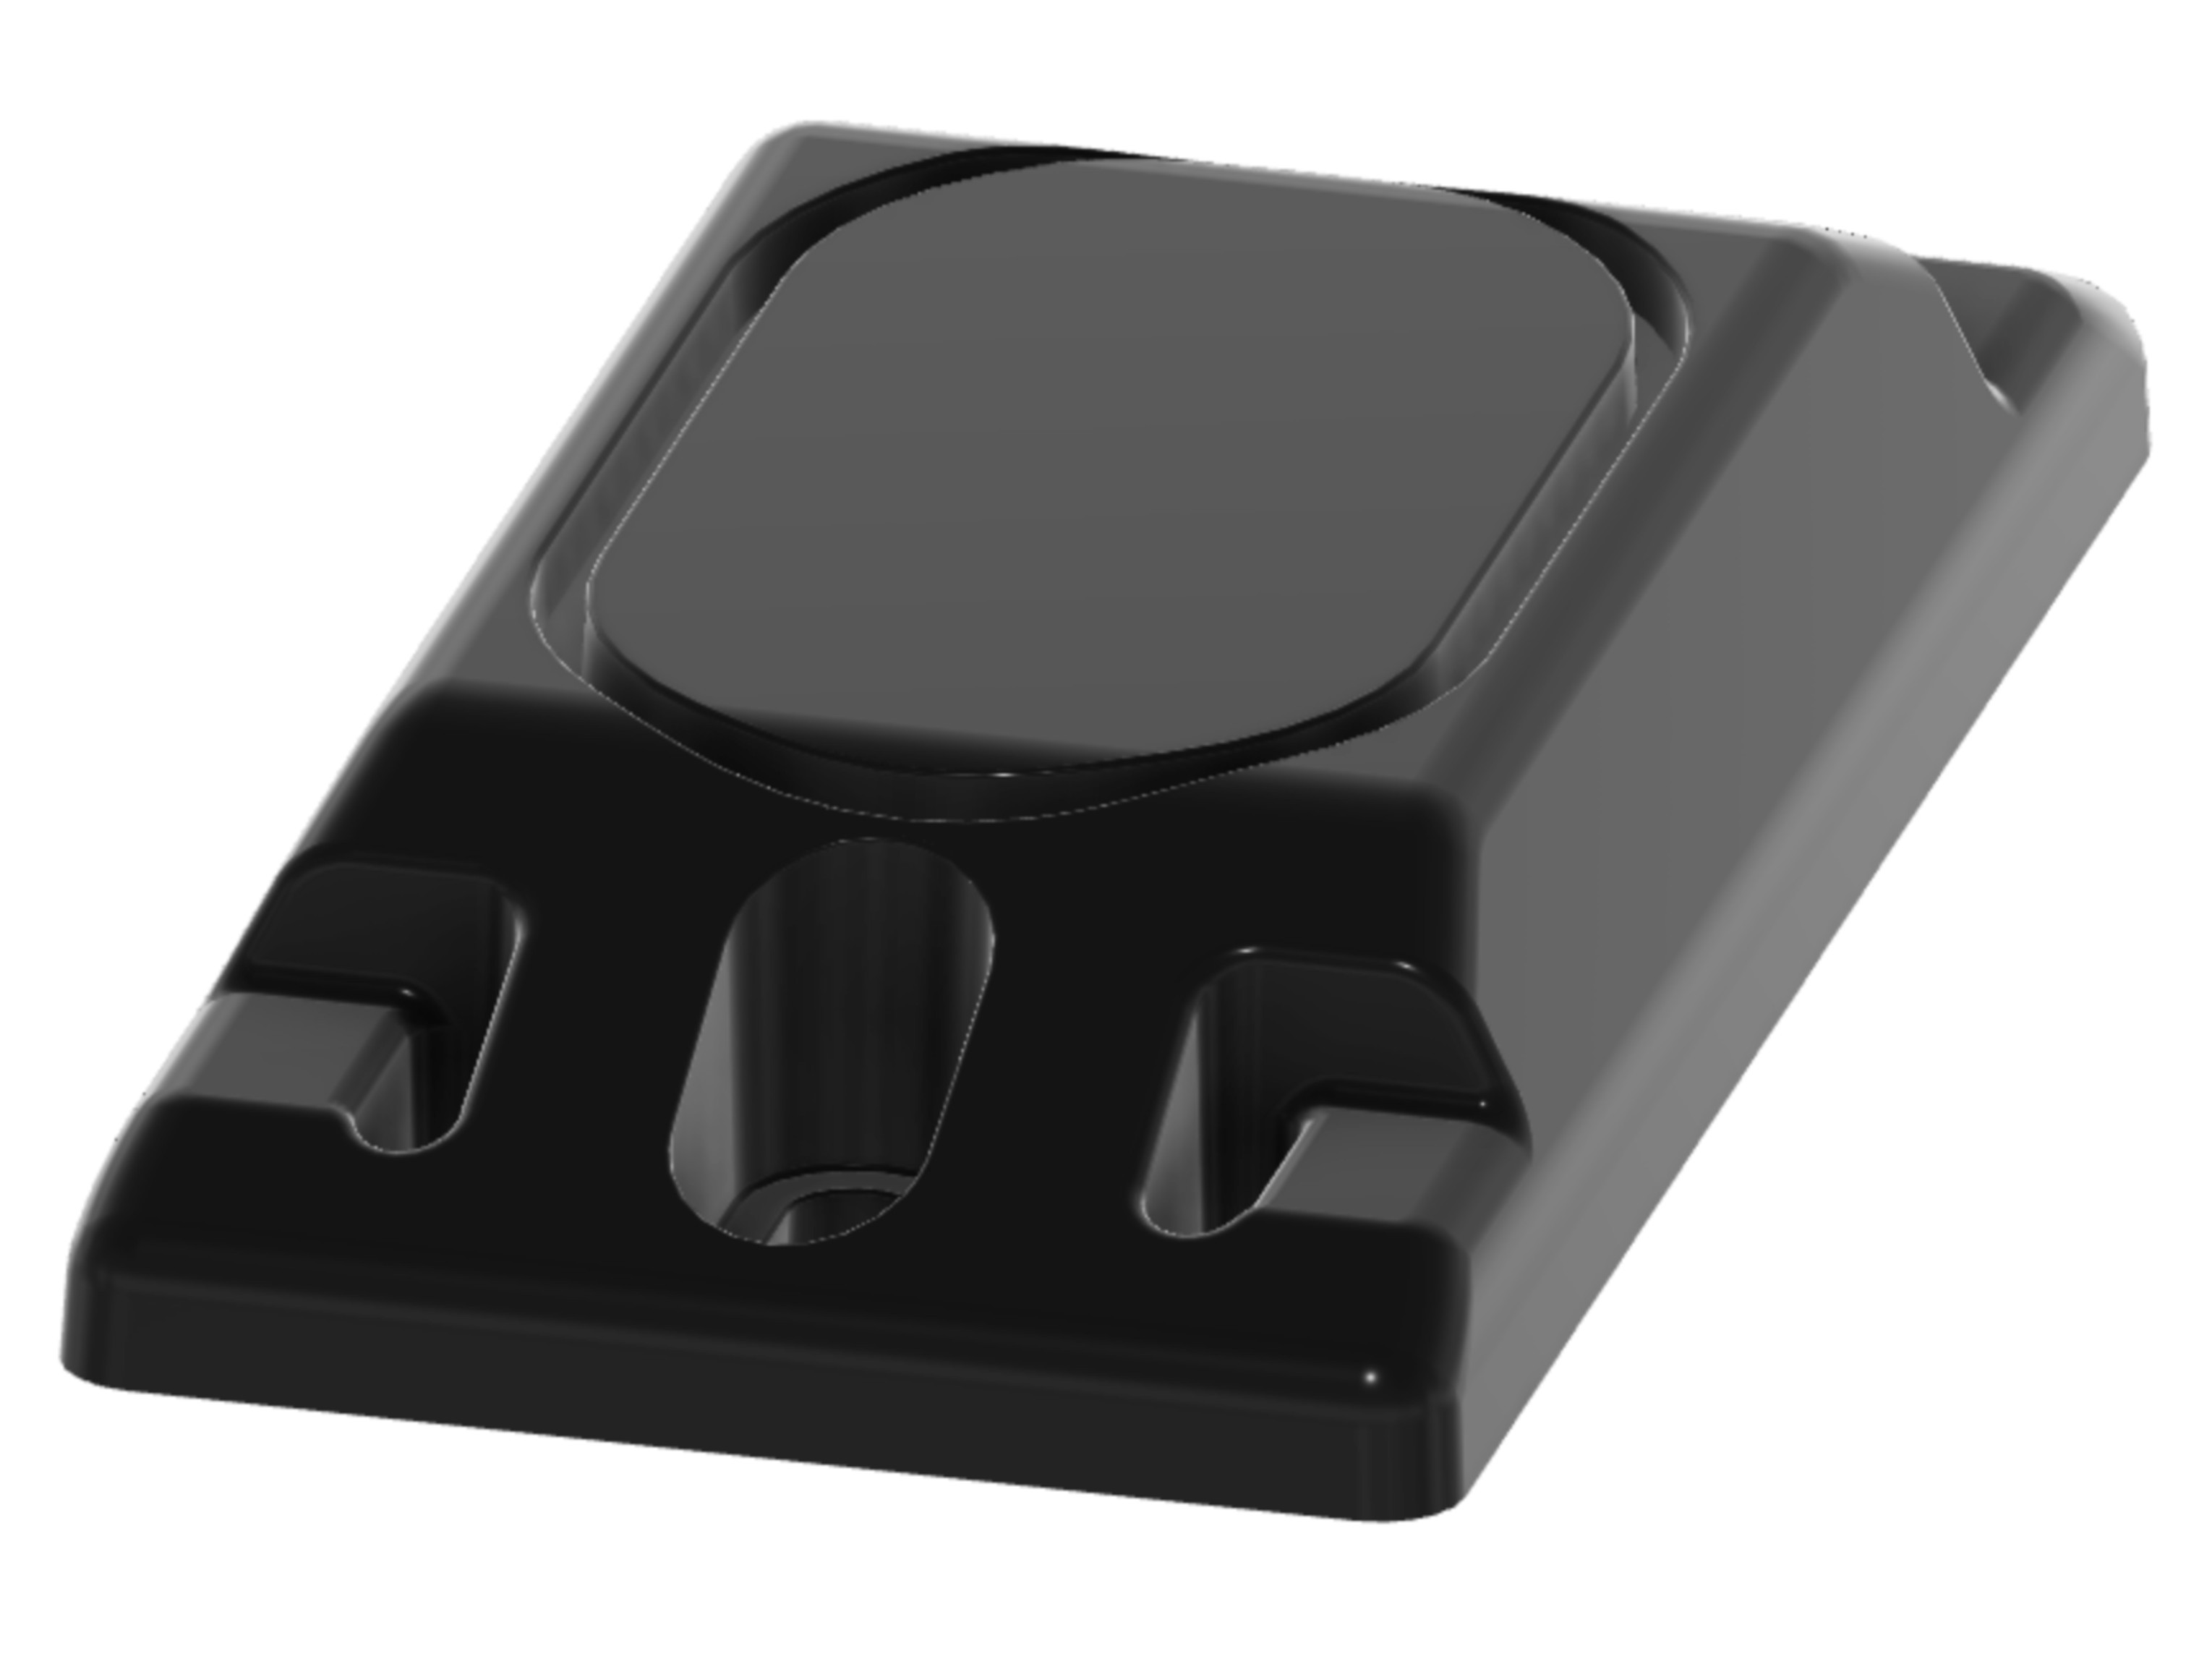
\includegraphics[width=5.5cm]{at_2}
\caption{Walkbase AT-2}
\label{fig:at2}
\end{figure}

\begin{figure}[H]
\centering
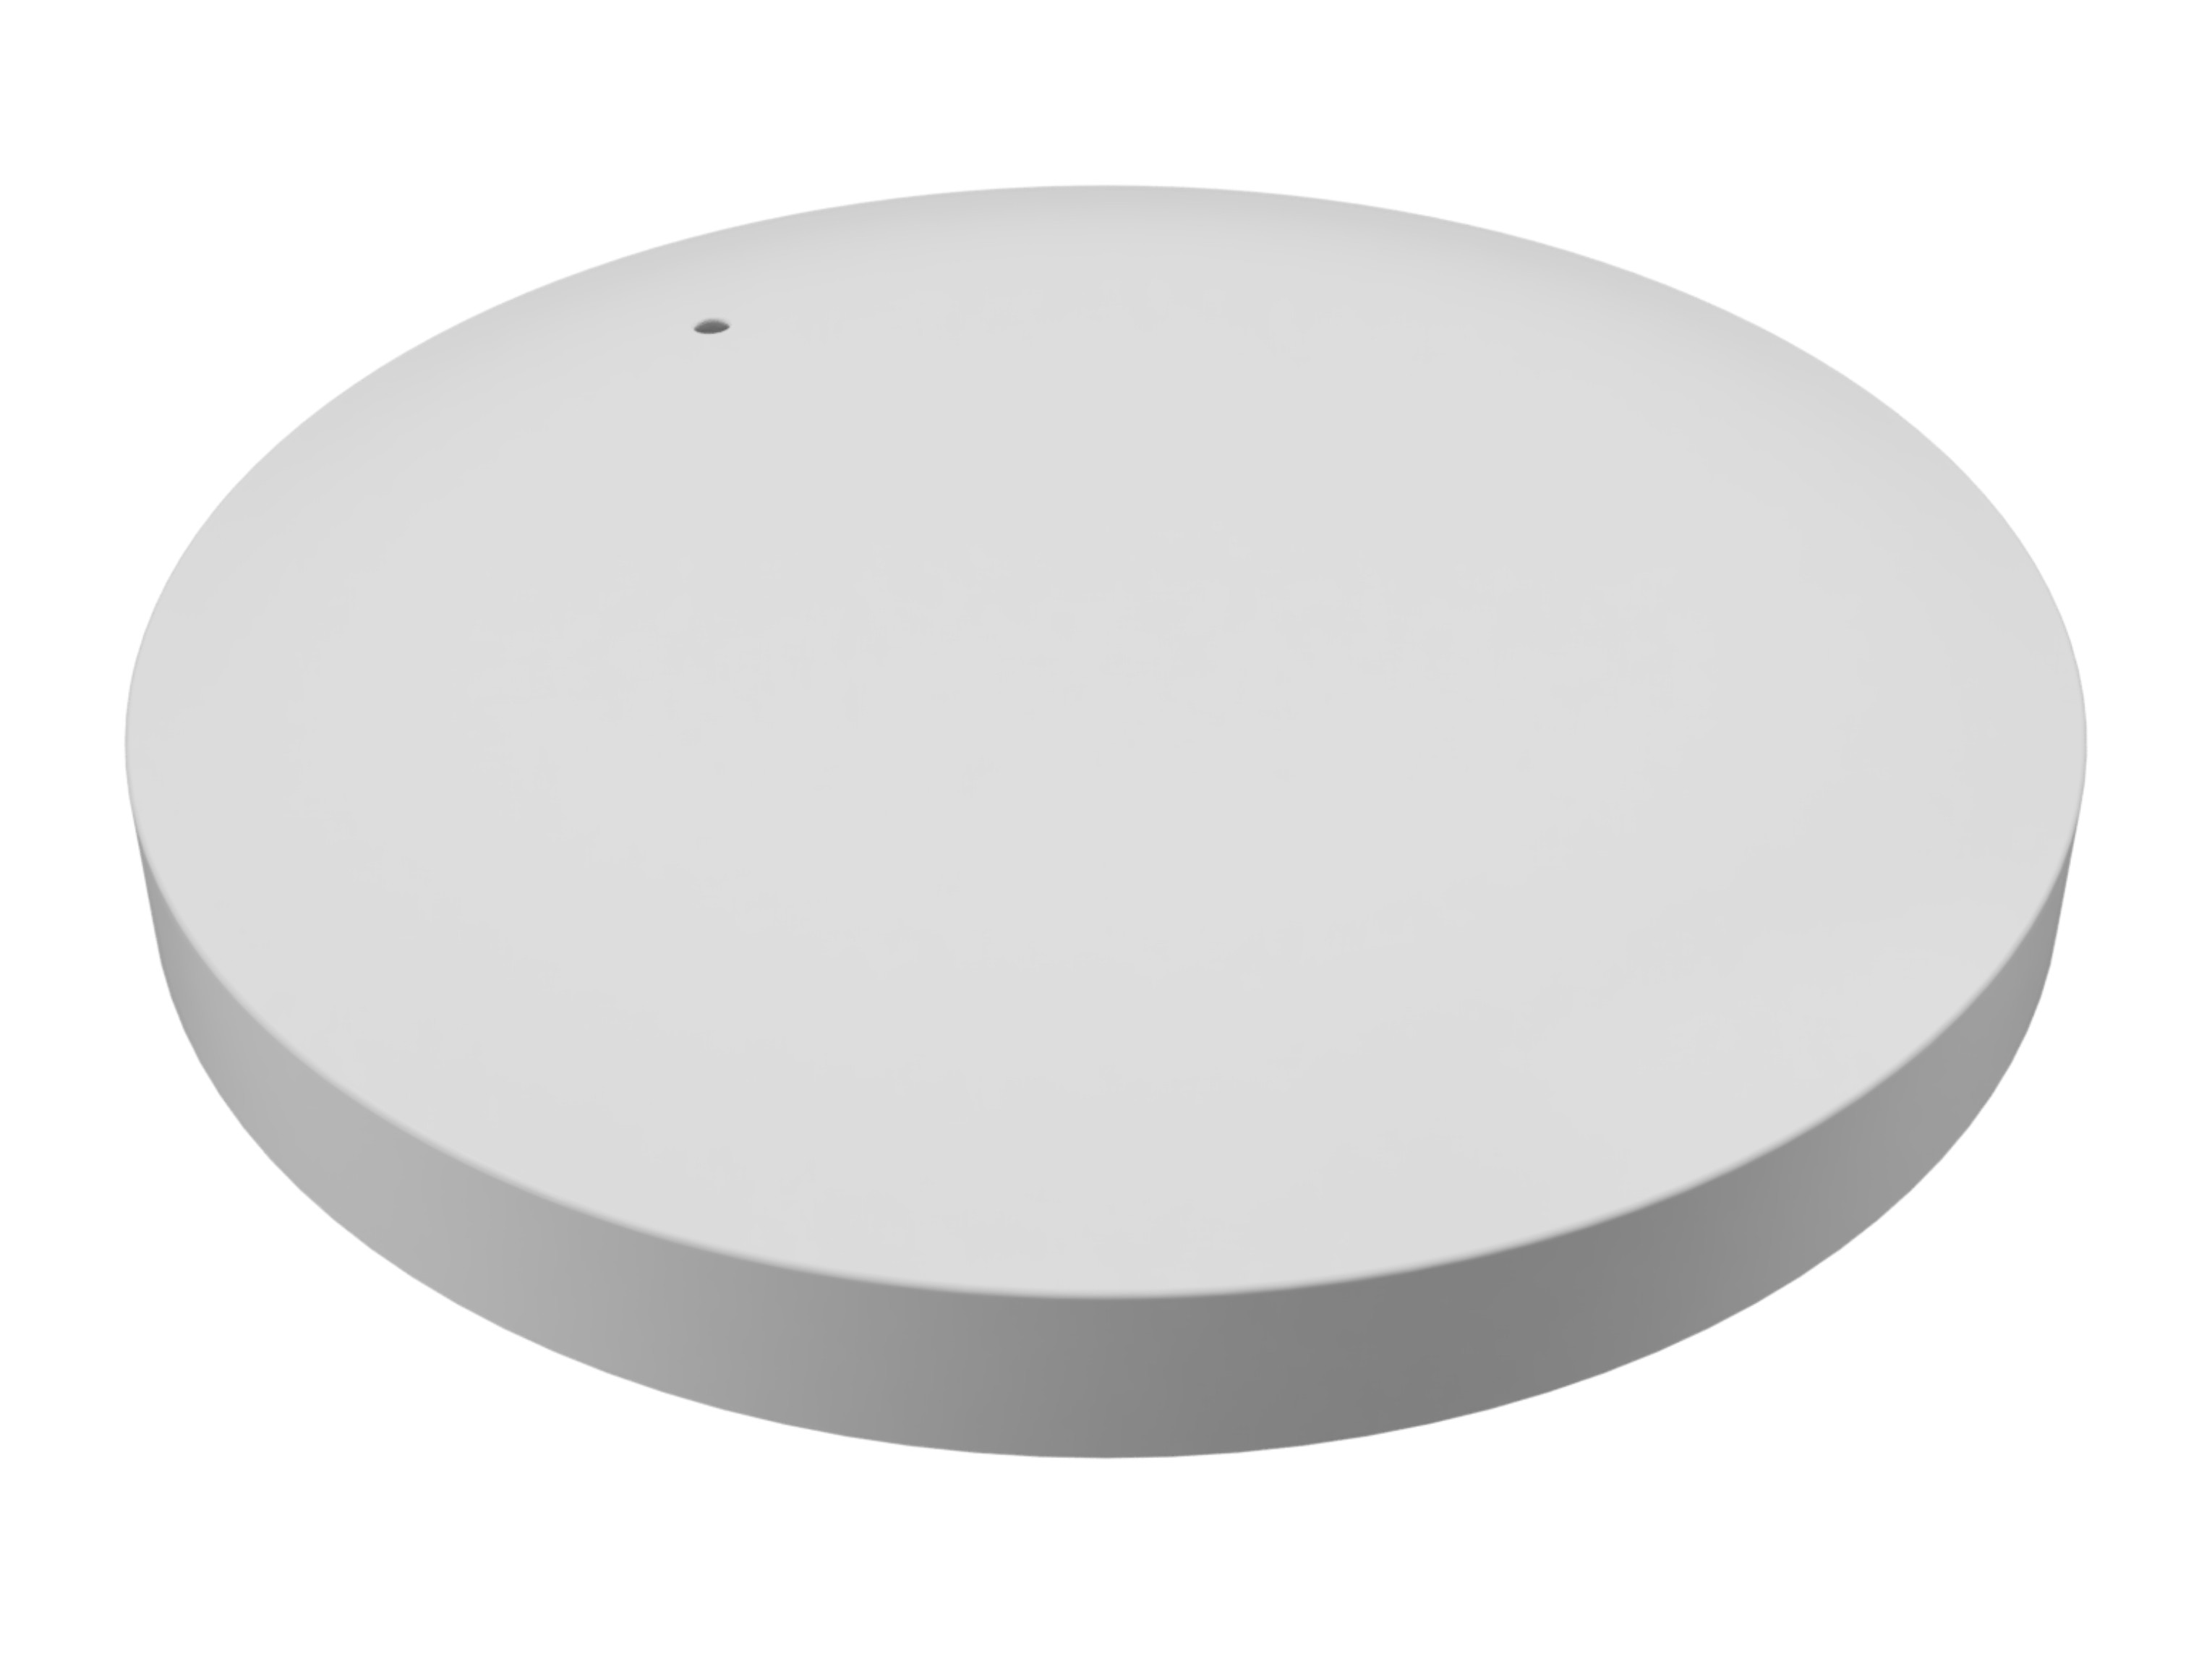
\includegraphics[width=5.5cm]{xr_2_plain}
\caption{Walkbase XR-2}
\label{fig:xr2}
\end{figure}
\end{multicols}

\begin{figure}[H]
\centering
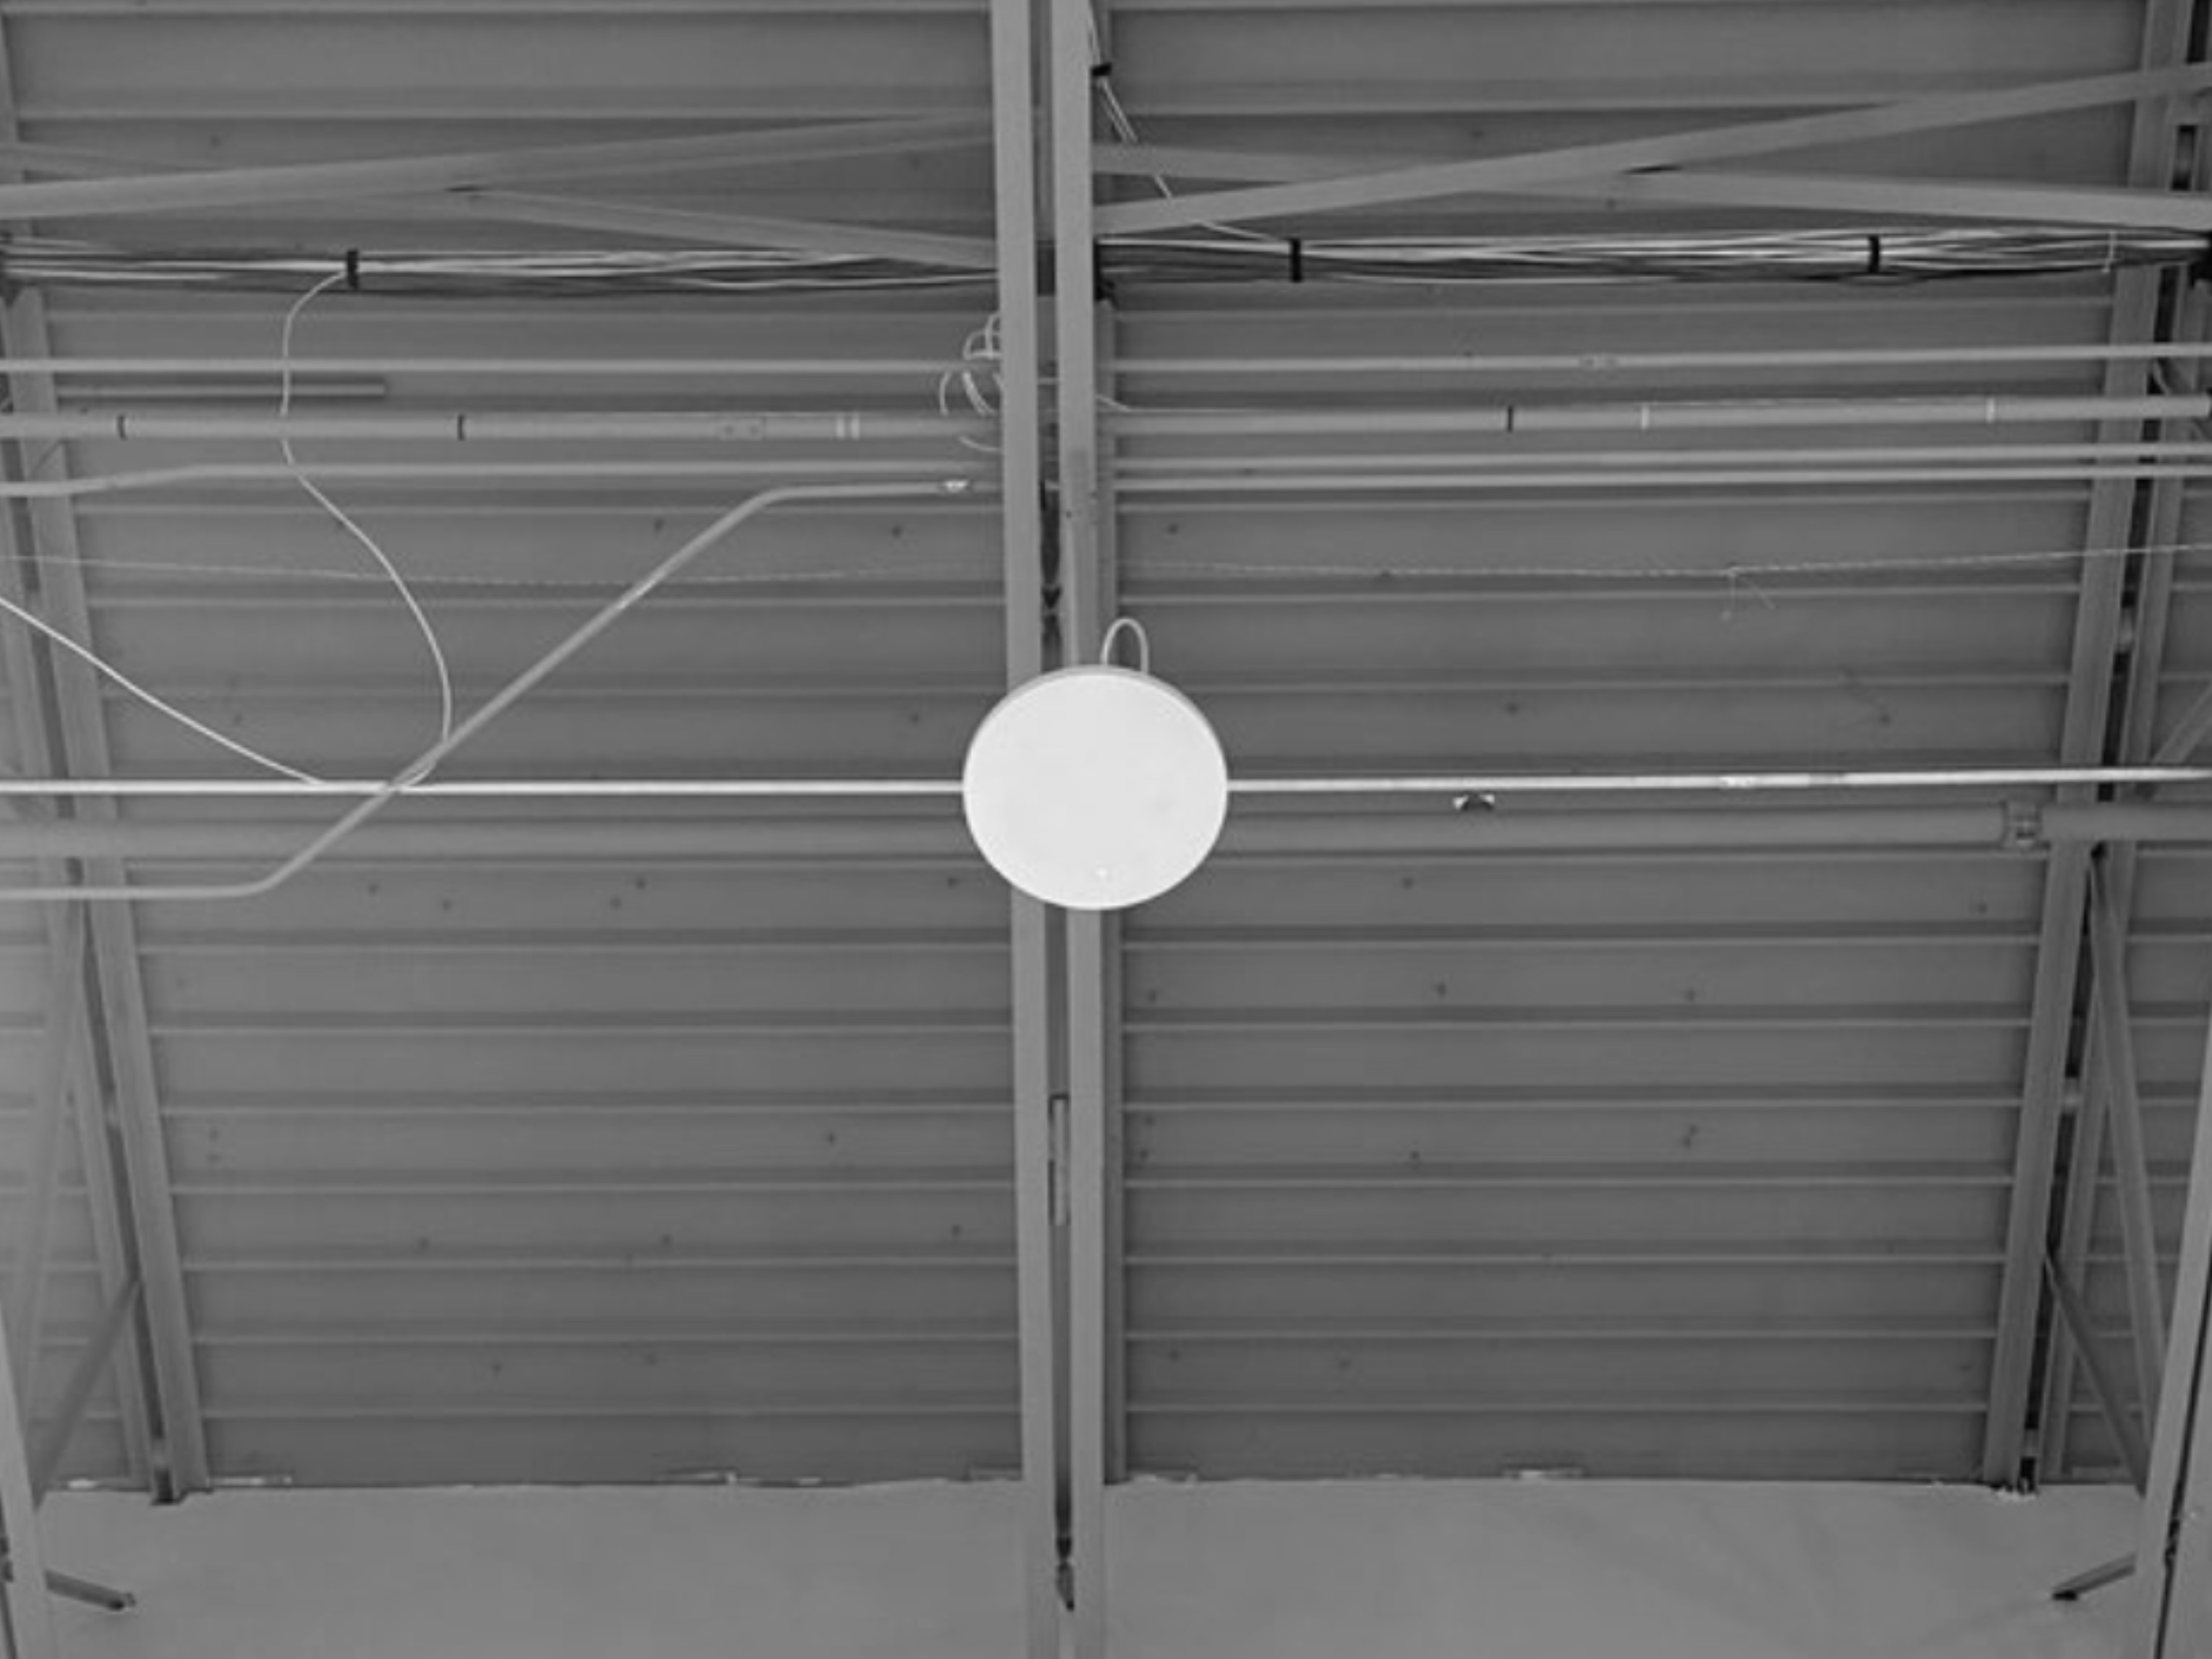
\includegraphics[width=5.5cm]{xr_2_installed}
\caption{Walkbase XR-2 asennettuna}
\label{fig:xr2_installed}
\end{figure}

Koeympäristön pohjapiirustus on esitetty kuvassa \ref{fig:testipolku}. Piirustuksessa XR-2-paikantimet on kuvattu punaisilla ympyröillä ja kuljettu testipolku on merkitty violetilla janalla. Piirustus luotiin käyttäen \texttt{ggplot2}-kirjastoa ja se löytyy RDS-muotoon tallennettuna osoitteesta \newline \url{https://github.com/rintakumpu/progradu/analyysi/R/data/sitemap.RDS}.

\begin{figure}[H]
\centering
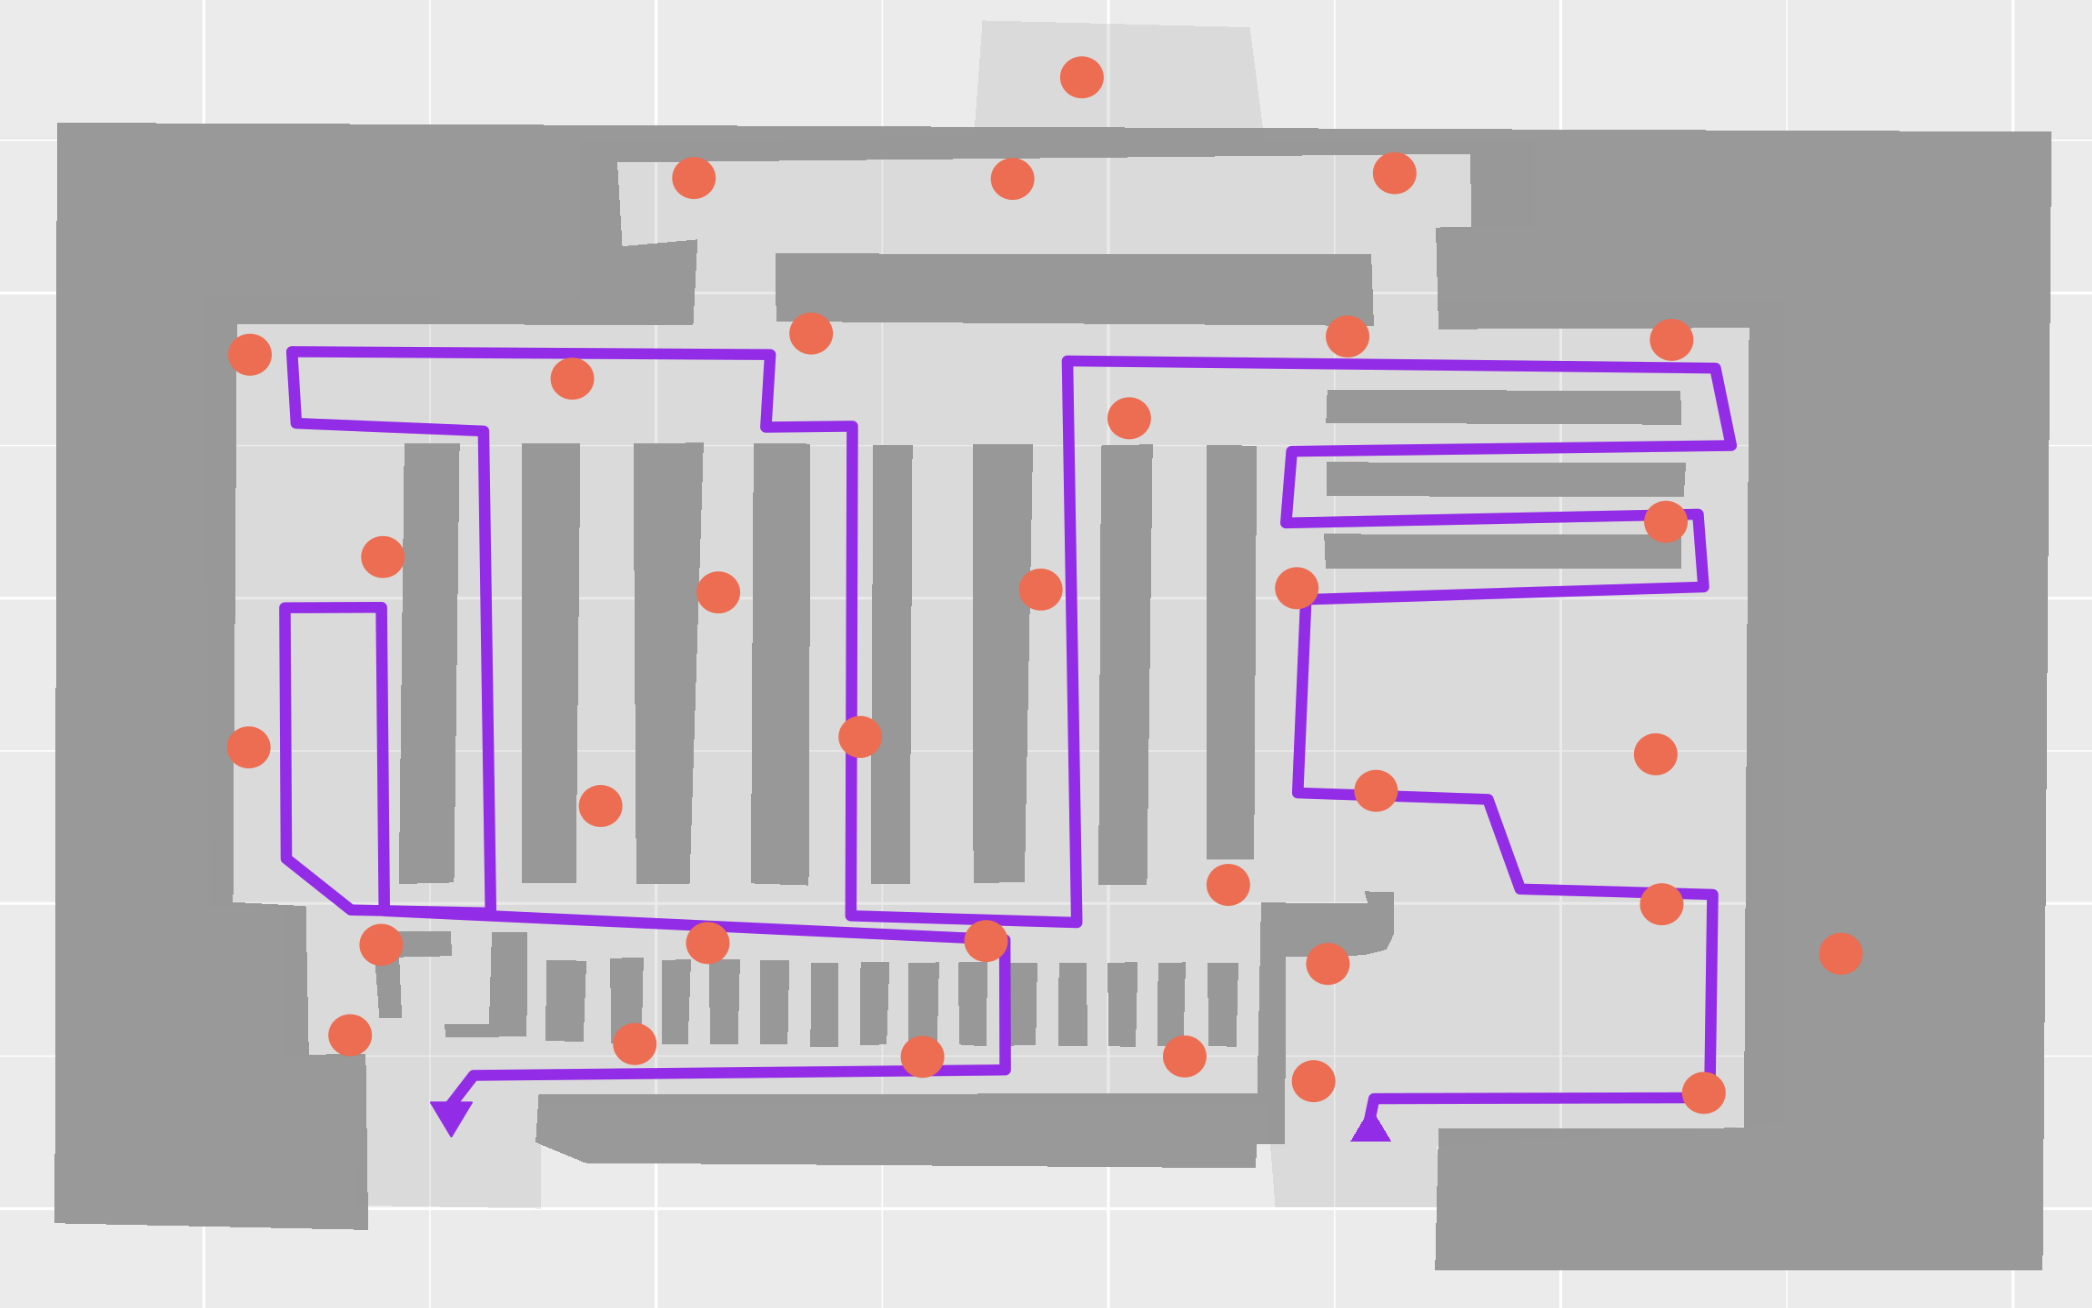
\includegraphics[width=15cm]{testipolku_numeroimaton}
\caption{Koeasetelman pohjapiirustus}
\label{fig:testipolku}
\end{figure}

\noindent Dataa kerättäessä AT-2-tagi kiinnitettiin ostoskärryyn 1.2 metrin korkeudelle (kts. kuvat \ref{fig:at2_cart} ja \ref{fig:at2_cart2}) ja testipolku käveltiin mahdollisimman tasaisella nopeudella. Data kerättiin aikaan, jolloin testiympäristön käyttöaste oli alhainen. Tällä minimoitiin radiosignaalien tielle osuvien ihmisten vaikutus signaaleihin. Kerätty tulokulmadata löytyy osoitteesta\newline \url{https://github.com/rintakumpu/progradu/analyysi/data/y.csv}. Pohjapiirustus- ja polkudata löytyvät osoitteista\newline \url{https://github.com/rintakumpu/progradu/analyysi/data/exclusion_polygons.csv} (ekskluusiopolygonit),\newline \url{https://github.com/rintakumpu/progradu/analyysi/data/inclusion_polygons.csv} (lattiapolygoni) ja\newline \url{https://github.com/rintakumpu/progradu/analyysi/data/test_path.csv} (testipolku). Datassa koordinaatit on valmiiksi interpoloitu metreiksi, jotta testiympäristön sijaintia ei voi paikallistaa koordinaattien perusteella. Interpolointiin käytetty ohjelmakoodi löytyy osoitteesta \newline \url{https://github.com/rintakumpu/progradu/analyysi/R/interpolate_coordinates.R} . Osoitteesta\newline \url{https://github.com/rintakumpu/progradu/analyysi/analyysi.Rmd} löytyy itse analyysikoodin sisältävä R Markdown -muistikirja.

\newpage

\begin{multicols}{2}
\begin{figure}[H]
\centering
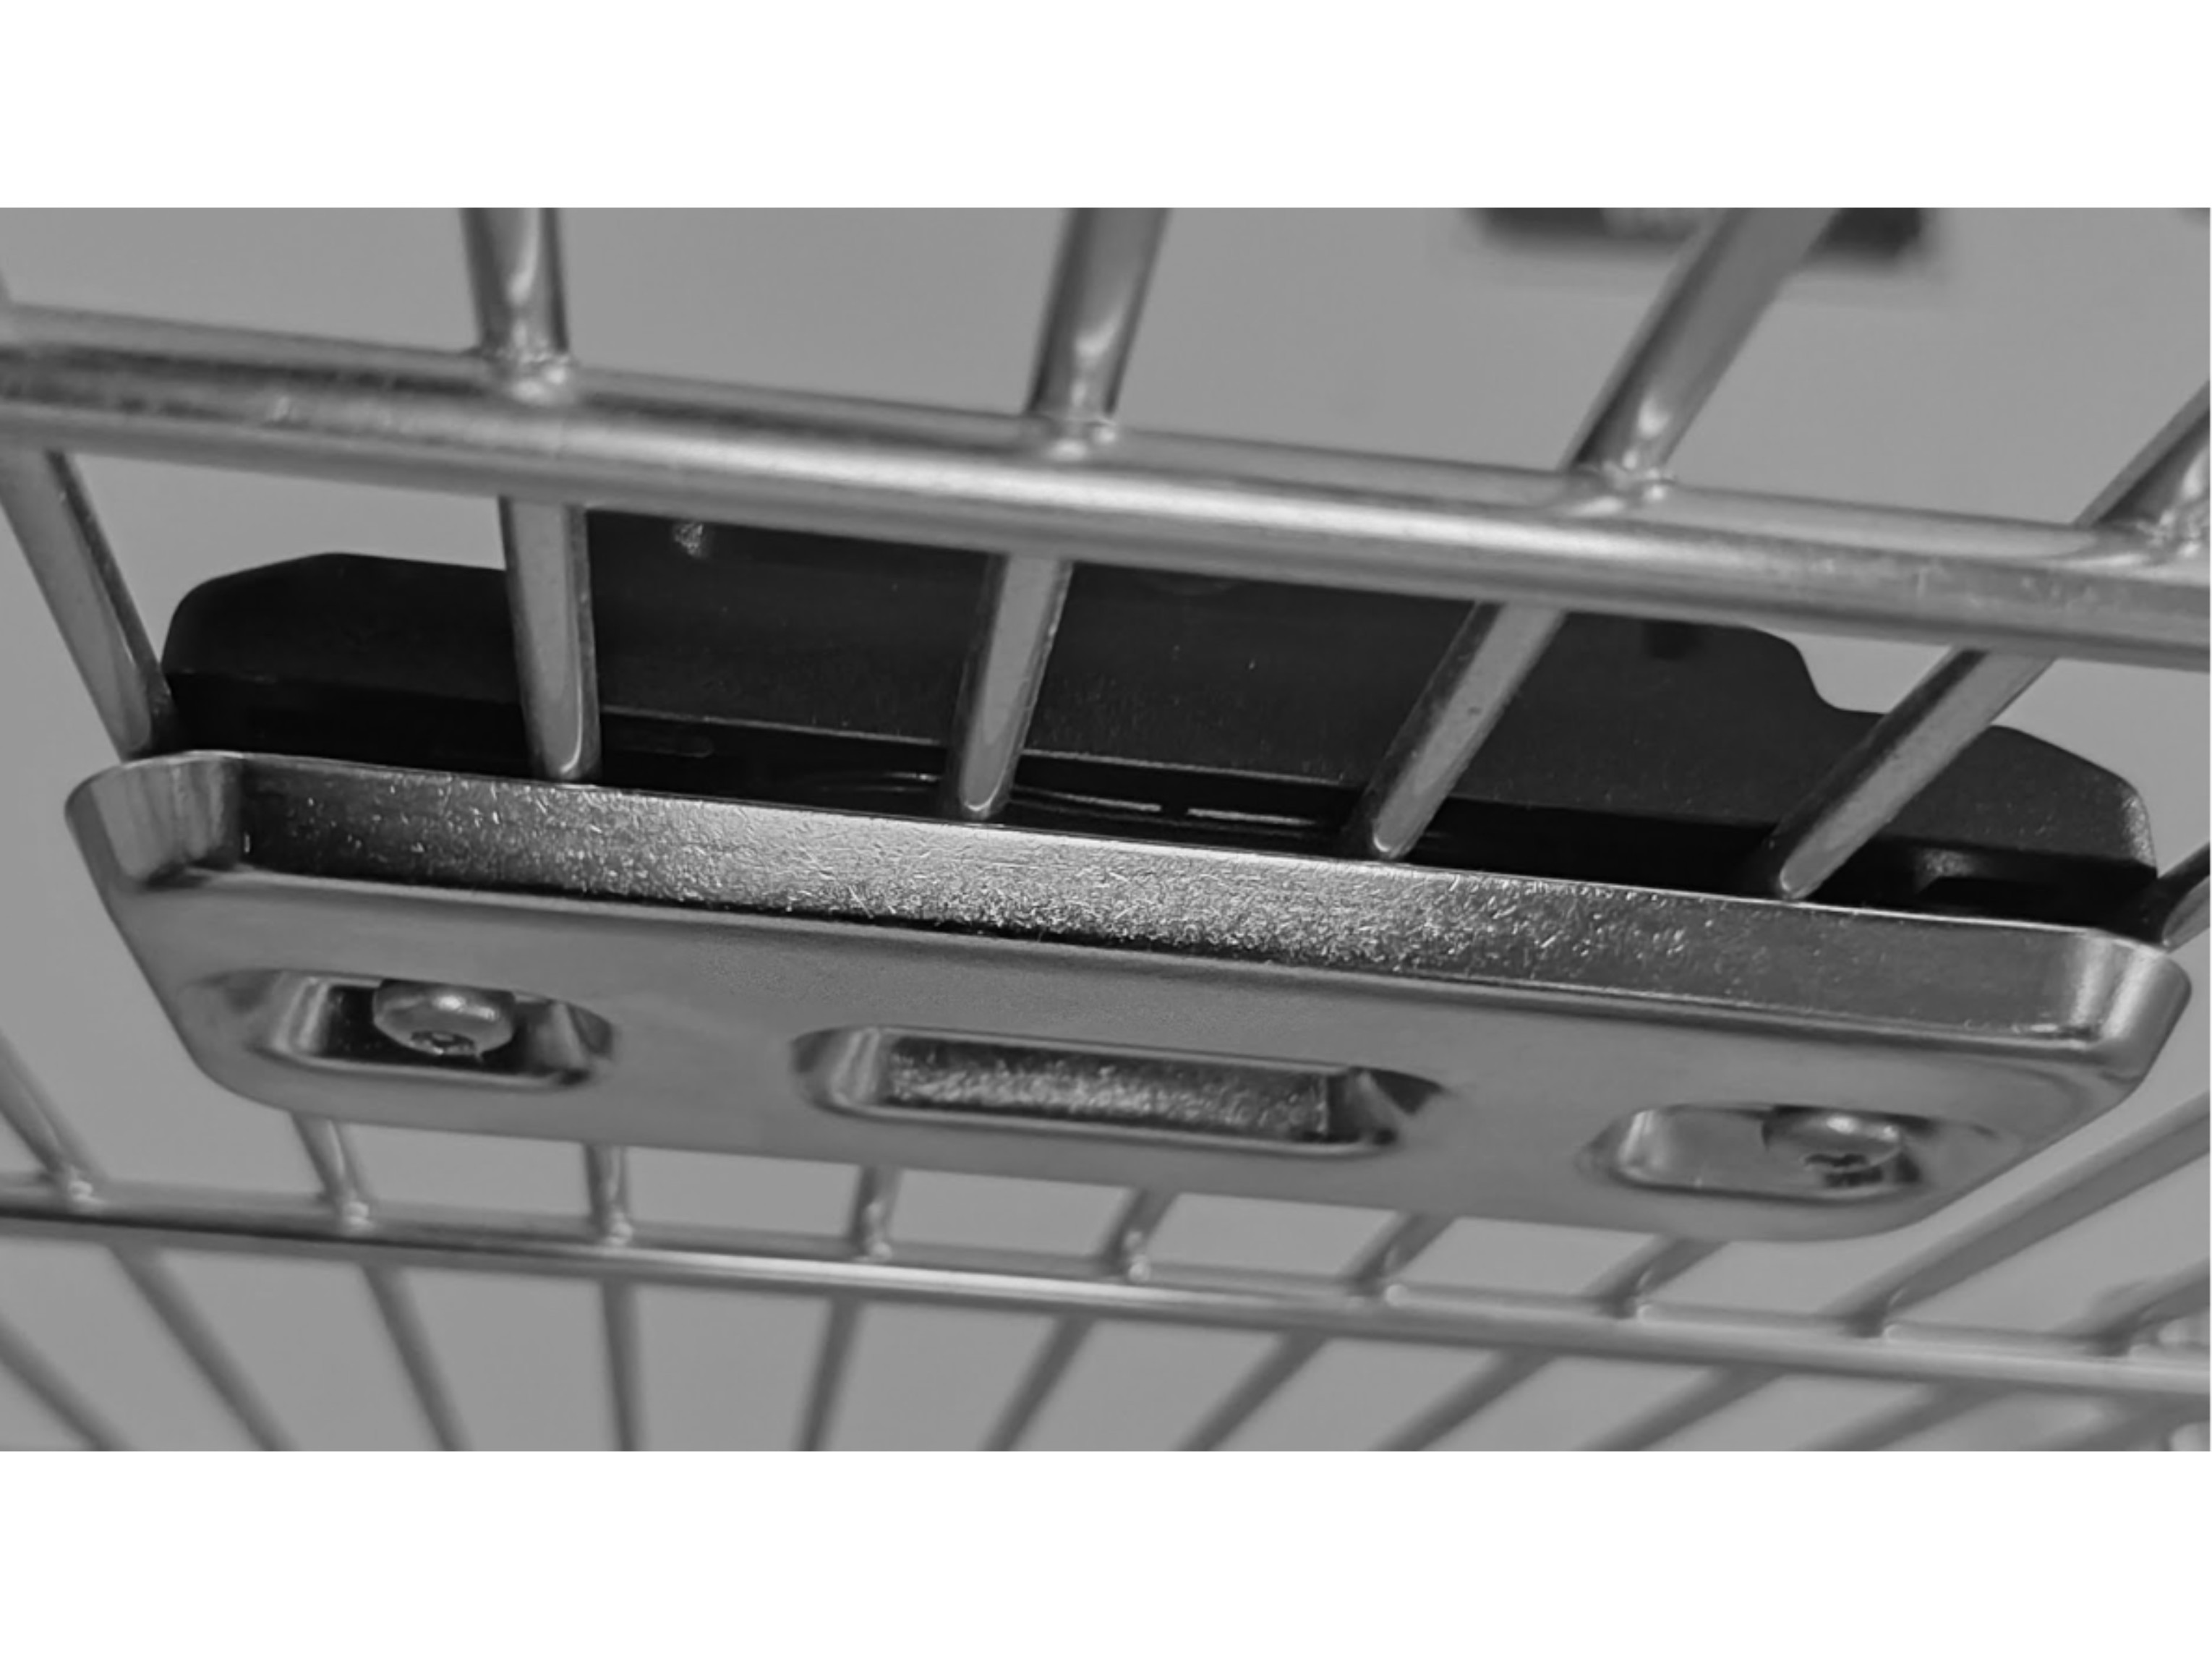
\includegraphics[width=5.5cm]{at_2_cart}
\caption{Walkbase AT-2 kiinnitettynä}
\label{fig:at2_cart}
\end{figure}

\begin{figure}[H]
\centering
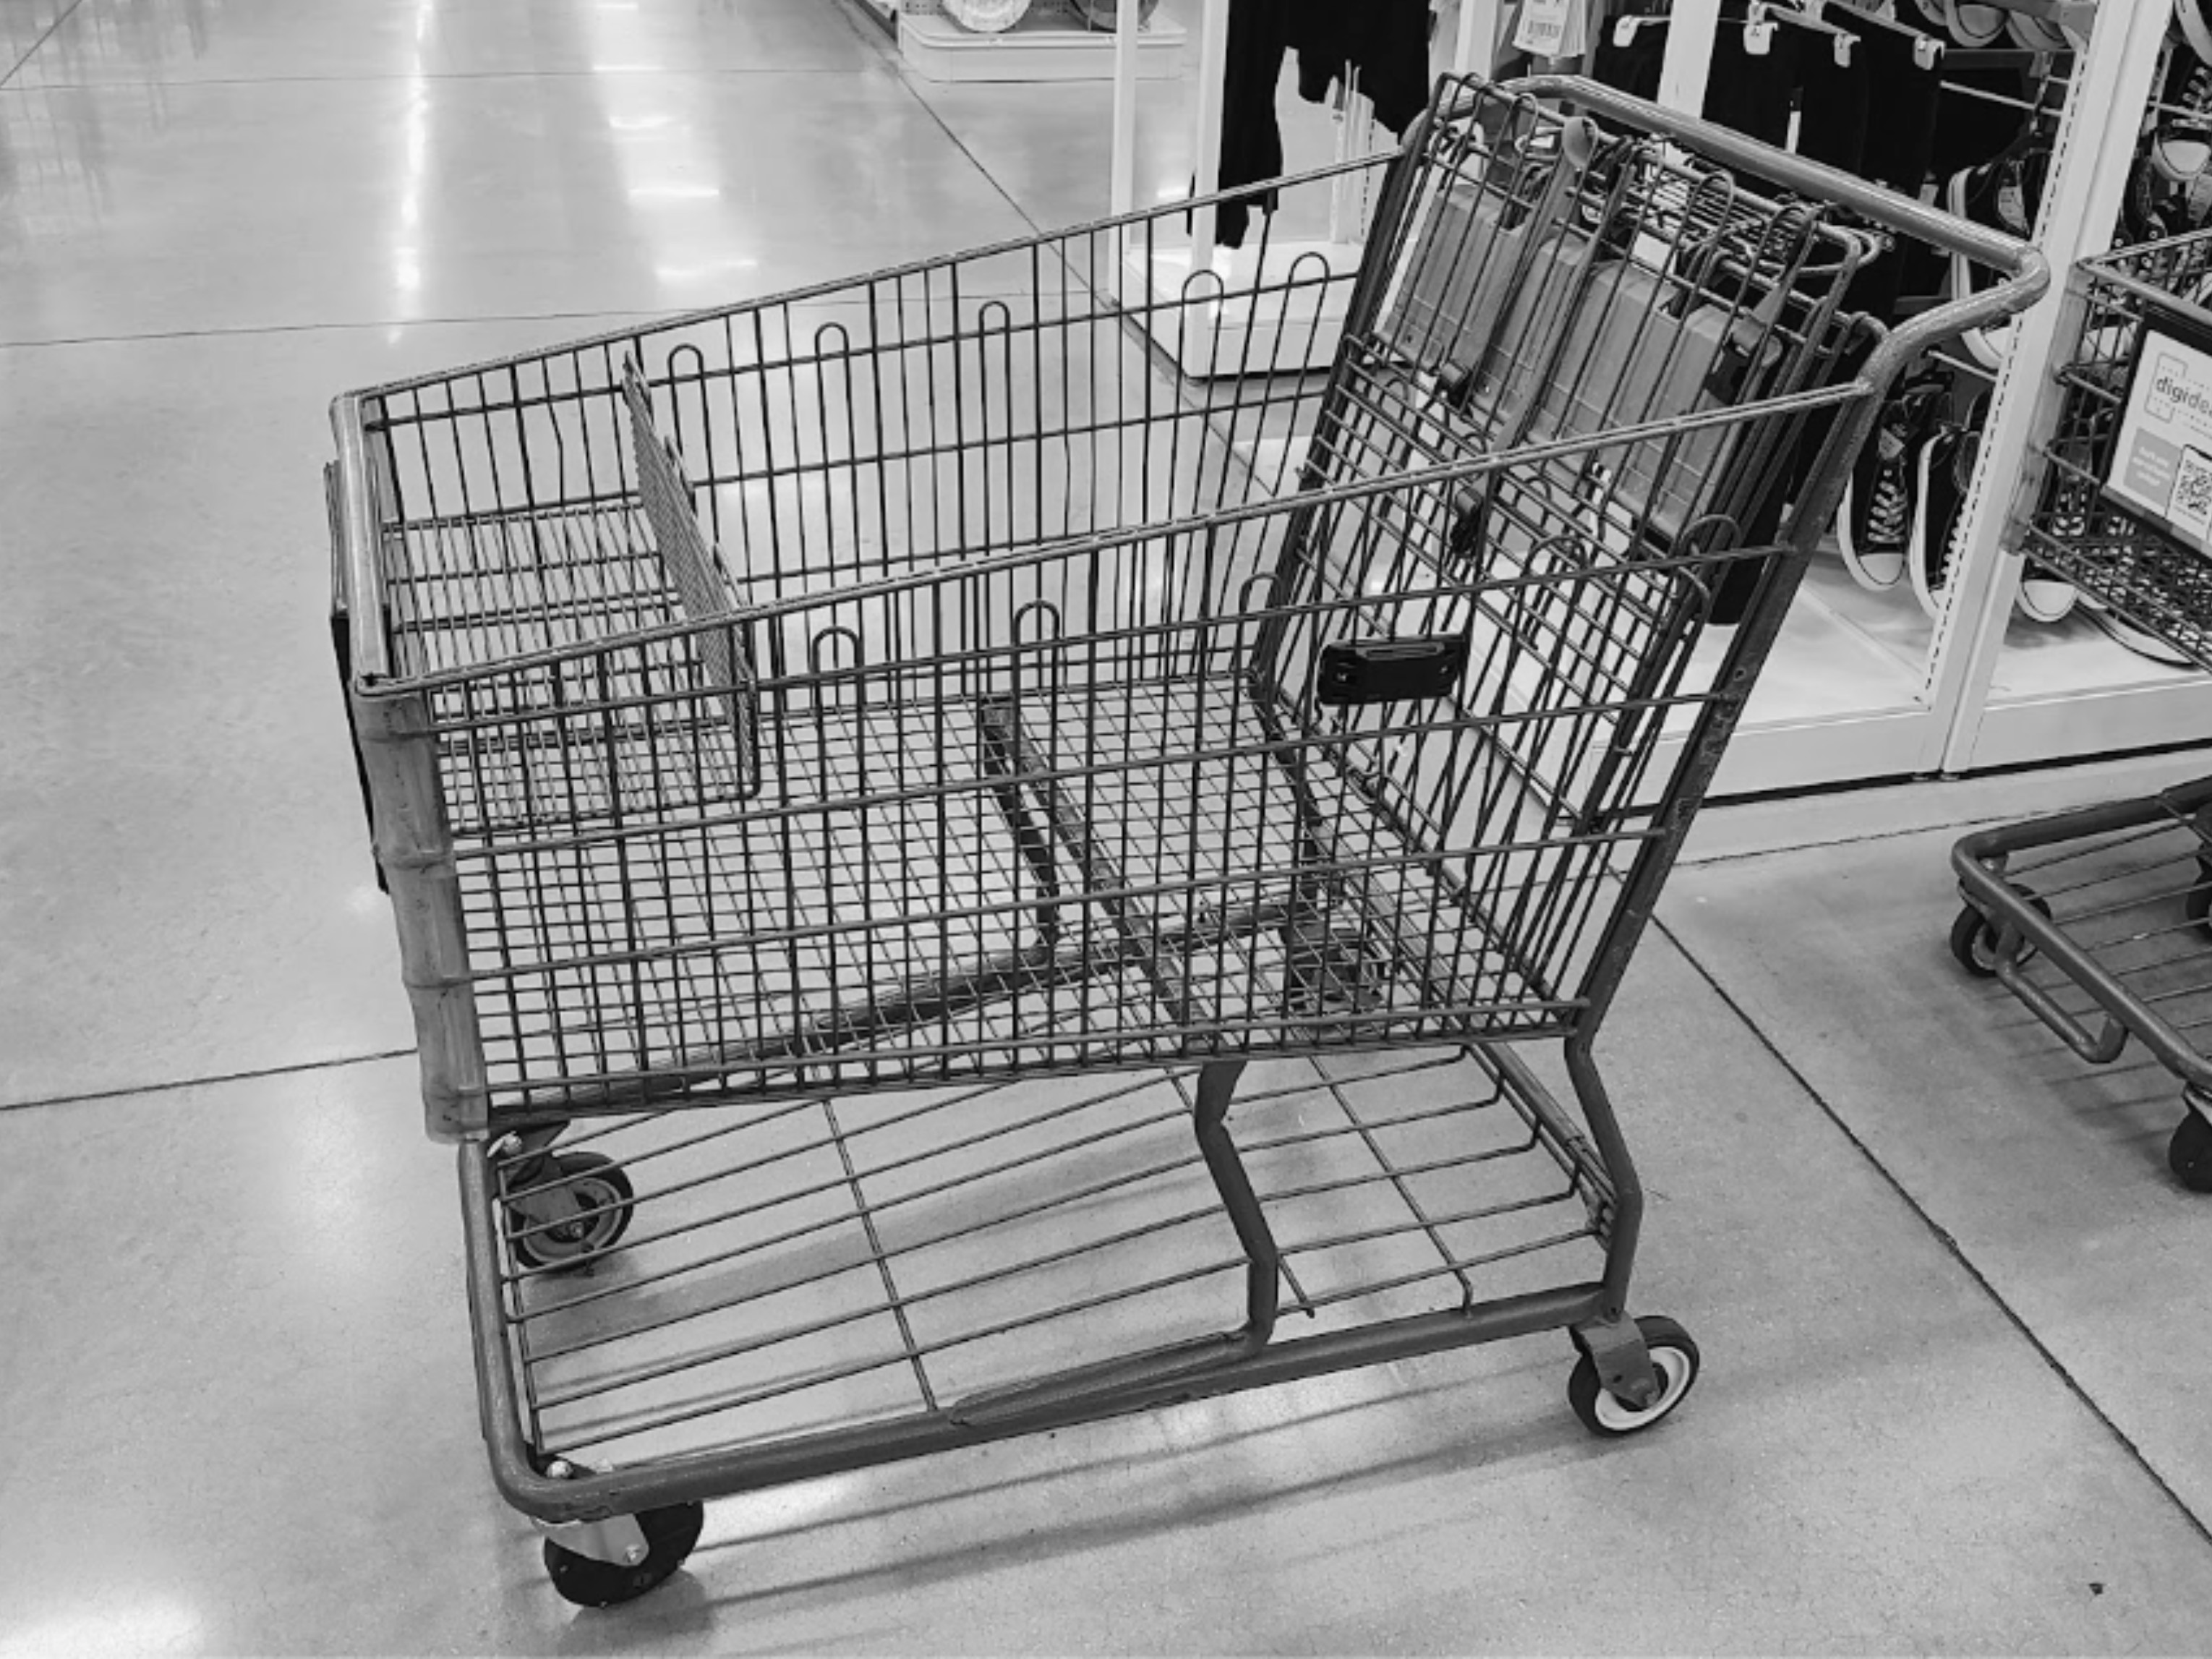
\includegraphics[width=5.5cm]{at_2_cart2}
\caption{Walkbase AT-2 kiinnitettynä}
\label{fig:at2_cart2}
\end{figure}
\end{multicols}

\subsection{Parametrien valinta} \label{parametrien-valinta}

Kokeessa oli tarkoituksena testata kunkin taulukossa \ref{tab:wb-parametrit} esitetyn parametrin vaikutusta algoritmin paikannusvirheeseen, ajoaikaan sekä varianssiin. Koska kaikkien parametrikombinaatioiden testaaminen ei ollut mahdollista (eikä mielekästä), suoritettiin kerättyyn dataan perustuva paikannus kolmessa vaiheessa. Kussakin vaiheessa paikannusalgoritmi ajettiin jokaisella vaiheeseen liittyvällä suunnitteluparametrikombinaatiolla \(r=30\) kertaa ja tulokset laskettiin näiden \(30\) ajon aritmeettisena keskiarvona.

Ensimmäisessä vaiheessa tarkasteltiin partikkelien määrän \(N={100,1000,10000}\) sekä uudelleenotannan kynnysarvon \(resampling={0,1/10,2/3,1}\) vaikutusta paikannuskeskivirheeseen. Karttasovitusalgoritmia ei käytetty, kuten ei myöskään prediktiivistä siloitinta eikä signaalin vahvuuden kynnysarvoa. Dynaamisen mallin kohina-arvo \(q=2\) pidettiin vakiona. Ensimmäisessä vaiheessa tarkasteltiin siis \(12\) eri suunnitteluparametrikombinaatiota.

Toisessa vaiheessa valittiin ensimmäisen vaiheen tulosten perusteella parhaimman paikannusvirheen suhteessa suoritusaikaan ja varianssiin tuottava uudelleenotannan kynnysarvo \(resampling\) sekä partikkelien määrä \(N\). Nämä pidettiin vakioarvoisina ja testattiin karttasovitusalgoritmia \emph{map\_matching} \(={T,F}\), karttasovitusalgoritmin rangaistusarvoa \(P={1,100,1000}\) sekä dynaamisen mallin kohina-arvoa \(q={0.75,1.5,2,2.5}\). Signaalin vahvuuden kynnysarvoa ei käytetty, kuten ei käytetty myöskään prediktiivistä siloitinta. Koska rangaistusarvo \(P\) oli käytössä ainoastaan karttasovitusalgoritmia käytettäessä, tarkasteltiin toisessa vaiheessa \(16\) eri suunnitteluparametrikombinaatiota.

Viimeisessä vaiheessa valittiin edellisten vaihdeiden tulosten perusteella parhaimman paikannusvirheen suhteessa suoritusaikaan ja varianssiin tuottavat parametrit testattujen joukosta ja testattiin datan valinnassa käytettävää signaalin vahvuuden kynnysarvoa \emph{rssi\_threshold} \(={-100,-90,-80}\) sekä prediktiivistä siloitinta \emph{smoothing} \(={T,F}\) eli kuutta eri suunnitteluparametrikombinaatiota.

Tulosten vertailukohtana käytettiin Pierlot \&al.~artikkelissa ``A New Three Object Triangulation Algorithm Based on the Power Center of Three Circles'' (2011) esittämää ToTal-triangulaatioalgoritmia \citep{Pierlot-2011}. Triangulaatio-algoritmia ei käsitellä tässä tarkemmin, mutta se on esitetty algoritmissa \(\ref{total}\). Algoritmia varten valittiin kullakin aika-askeleella \(k\) ne kolme XR-2-laitetta ja kulmahavaintoa, joiden RSSI-arvo oli korkein. Käytetty algoritmin toteutus löytyy osoitteesta \newline  \url{https://github.com/rintakumpu/progradu/analyysi/R/total.R}.

Paikannusalgoritmi ajettiin RStudion versiossa 2023.09.0+463 R-ohjelmointikielen versiolla 4.2.0. Tietokoneena käytettiin vuoden 2021 mallia olevaa MacBook Pro -kannettavaa, jossa oli Apple M1 Pro -prosessori sekä 32 gigatavua LPDDR5-muistia. Suoritusnopeuden mittaamiseen käytettiin \texttt{Sys.time()}-funktiota.

\begin{algorithm}[H]
\label{total}
\DontPrintSemicolon
\SetAlgoShortEnd
\KwResult{Testilaitteen sijaintiestimaatti $(x_R,y_R)$.\;}
\KwData{Kolmen paikantimen koordinaatit $(x_i,y_i)$, $i=\{1,2,3\}$ ja näitä vastaavat vastakkaiset kulmahavainnot $\Phi^\prime_1, \Phi^\prime_2, \Phi^\prime_3$.\;}
\Begin{Lasketaan muokatut koordinaatit \newline
$x^\prime_1=x_1-x_2, \hspace{0.5cm} y^\prime_1=y_1-y_2, \hspace{0.5cm} x^\prime_3=x_3-x_2, \hspace{0.5cm} y^\prime_3=y_3-y_2.$ \;}
\Begin{Lasketaan kotangentit \newline
$T_{12}=\cot(\Phi^\prime_2-\Phi^\prime_1), \hspace{0.5cm} T_{23}=\cot(\Phi^\prime_3-\Phi^\prime_2), \hspace{0.5cm}T_{31}=\frac{1-T_{12}T_{23}}{T_{12}+T_{23}}$.\;}
\Begin{Lasketaan muokatut ympyröiden keskipisteet $(x^\prime_{ij},y^\prime_{ij})$ \newline
$x^\prime_{12}=x^\prime_1+T_{12}y^\prime_1,\hspace{0.5cm}y^\prime_{12}=y^\prime_1-T_{12}x^\prime_1$ \newline $x^\prime_{23}=x^\prime_3-T_{23}y^\prime_3,\hspace{0.5cm}y^\prime_{23}=y^\prime_3+T_{23}x^\prime_3$ \newline
$x^\prime_{31}=(x^\prime_3+x^\prime_1)+T_{31}(y^\prime_3-y^\prime_1),\hspace{0.5cm}y^\prime_{31}=(y^\prime_3+y^\prime_1)-T_{31}(x^\prime_3-x^\prime_1)$.
\;}
\Begin{Lasketaan $k^\prime_{31}=x^\prime_1x^\prime_3+y^\prime_1y^\prime_3+T_{31}(x^\prime_1y^\prime_3-x^\prime_3y^\prime_1).$\;}
\Begin{Lasketaan nimittäjä $D$ (jos $D=0$ palautetaan virhe).\newline
$D=(x^\prime_{12}-x^\prime_{23})(y^\prime_{23}-y^\prime_{31})-(y^\prime_{12}-y^\prime_{23})(x^\prime_{23}-x^\prime_{31})$.\;}
\Begin{Lasketaan ja palautetaan sijaintiestimaatti $(x_R,y_R)$. \newline
$x_R=x_2+\frac{k^\prime_{31}(y^\prime_{12}-y^\prime_{23})}{D}\hspace{0.5cm}y_R=y_2+\frac{k^\prime_{31}(x^\prime_{23}-x^\prime_{12})}{D}$.\;}
\caption{ToTal (Three object Triangulation algorithm)}
\end{algorithm}

\hypertarget{tulokset}{%
\subsection{Tulokset}\label{tulokset}}

Ensimmäisessä vaiheessa suoritettiin paikannus partikkelien määrällä \(N={100,1000,10000}\) sekä uudelleenotannan kynnysarvolla \(resampling={0,1/10,2/3,1}\). Kun kynnysarvo oli \(0\), uudelleenotantaa ei käytetty, jolloin SIR-algoritmin sijaan paikannus suoritettiin SIS-algoritmilla. Kun kynnysarvo oli \(1\), uudelleenotanta suoritettiin jokaisella aika-askeleella. Arvoilla \(1/10\) ja \(2/3\) käytettiin adaptiivista uudelleenotantaa. Tulokset on esitetty kuvassa \(\ref{fig:phase1-results}\) sekä taulukoissa \ref{tab:vaihe-1-tulokset} ja \ref{tab:vaihe-1-tulokset-varianssi}. Tulostaulukon sarake \(<1m\) kuvaa suurinta persentiiliä\(/100\), jolla saavutettiin haluttu metrin paikannusvirhe. Ajojen tulokset on esitetty karttapolkuina liitteen A alaluvussa \nameref{vaihe-1}.

\begin{table}

\caption{\label{tab:vaihe-1-tulokset}Vaiheen 1 tulokset, paikannusvirhe}
\centering
\begin{tabular}[t]{rrrlr}
\toprule
N & resampling & Mediaani (m) & Mediaanin 95\%-luottamusväli & <1m\\
\midrule
100 & 0.00 & 1.95 & {}[1.87, 2.03] & 0.28\\
1000 & 0.00 & 1.05 & {}[1.03, 1.07] & 0.48\\
10000 & 0.00 & 0.88 & {}[0.87, 0.88] & 0.55\\
100 & 0.10 & 0.86 & {}[0.86, 0.87] & 0.57\\
1000 & 0.10 & 0.86 & {}[0.86, 0.87] & 0.57\\
\addlinespace
10000 & 0.10 & 0.86 & {}[0.86, 0.86] & 0.58\\
100 & 0.67 & 0.88 & {}[0.87, 0.89] & 0.56\\
1000 & 0.67 & 0.86 & {}[0.86, 0.87] & 0.58\\
10000 & 0.67 & 0.86 & {}[0.86, 0.86] & 0.58\\
100 & 1.00 & 0.88 & {}[0.87, 0.89] & 0.56\\
\addlinespace
1000 & 1.00 & 0.86 & {}[0.86, 0.86] & 0.58\\
10000 & 1.00 & 0.86 & {}[0.86, 0.86] & 0.58\\
\bottomrule
\end{tabular}
\end{table}

\begin{table}

\caption{\label{tab:vaihe-1-tulokset-varianssi}Vaiheen 1 tulokset, varianssi ja ajoaika}
\centering
\begin{tabular}[t]{rrrrr}
\toprule
N & resampling & Varianssi & MC-varianssi & Ajoaika (s)\\
\midrule
100 & 0.00 & NA & 22.54 & 7.64\\
1000 & 0.00 & NA & 2.02 & 15.35\\
10000 & 0.00 & NA & 0.13 & 85.44\\
100 & 0.10 & 0.07 & 0.14 & 6.97\\
1000 & 0.10 & 0.00 & 0.03 & 14.40\\
\addlinespace
10000 & 0.10 & 0.00 & 0.01 & 82.68\\
100 & 0.67 & 0.06 & 0.09 & 7.16\\
1000 & 0.67 & 0.00 & 0.02 & 14.50\\
10000 & 0.67 & 0.00 & 0.00 & 81.78\\
100 & 1.00 & 0.06 & 0.09 & 7.19\\
\addlinespace
1000 & 1.00 & 0.00 & 0.02 & 14.48\\
10000 & 1.00 & 0.00 & 0.00 & 83.31\\
\bottomrule
\end{tabular}
\end{table}

\clearpage

\begin{figure}

{\centering 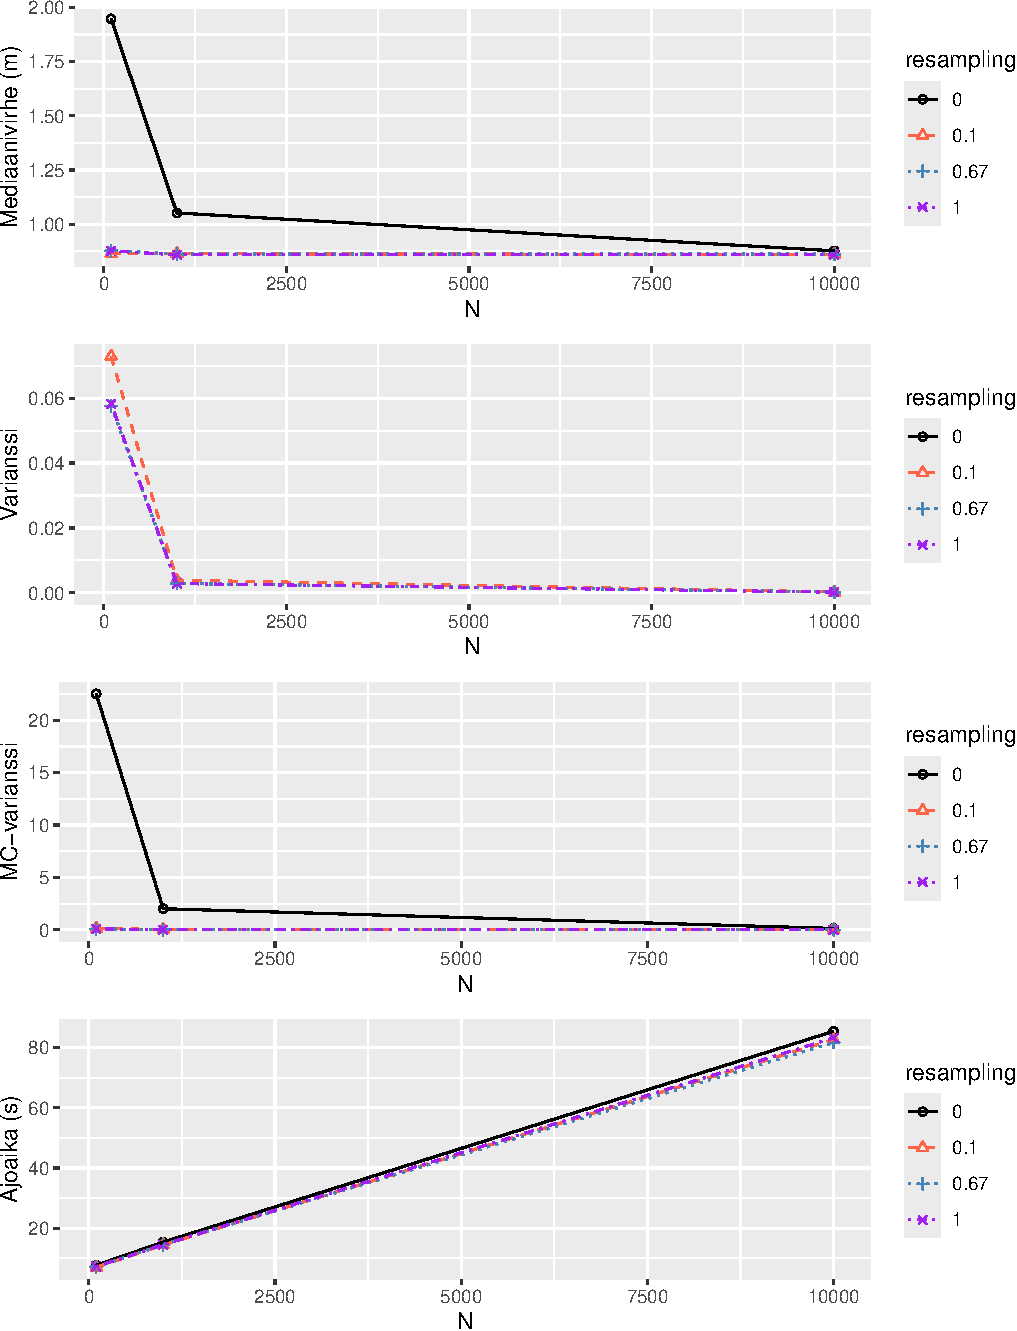
\includegraphics[width=15cm,height=20cm]{output/figures/phase1-results-1} 

}

\caption{Vaiheen 1 tulokset}\label{fig:phase1-results}
\end{figure}

Ensimmäisen vaiheen tuloksista huomataan, ettei hiukkasten määrällä ole juurikan vaikutusta mediaanipaikannusvirheesen, kun uudelleenotanta on käytössä (so. käytämme SIR-algoritmia). Samoin adaptiivisen uudelleenotannan kynnysarvolla ei ole juurikaan vaikutusta mediaanipaikannusvirheeseen.

Se, ettei partikkelien määrän kasvattaminen automaattisesti paranna paikannustarkkuuta viittaa siihen, että koeasetelma on herkkä priorijakauman valinnalle. Tuloksista huomataan lisäksi, että algoritmin aikakompleksisuus on uudelleenotannasta riipumatta luokkaa \(\mathcal{O}(N)\), kuten tukielman teoriaosassa todettiin. Samoin hiukkasten määrän kasvattaminen pienentää variansseja, kuten teoriaosassa todettiin.

Koska MC-varianssi on laskettu itse sijaintiestimaateista ja ALVar-varianssi kaikista partikkeleista, on näiden kahden varianssin suuruusluokka eri. Huomataan kuitenkin, että nämä kaksi varianssiestimaattia ovat hyvin korreloituneita, korrelaatiokertoimilla \(\rho_\text{Pearson} \approx 0.98\) ja \(\rho_\text{Spearman} \approx 0.97\). Voidaan siis olettaa ALVar-varianssin estimoivan hyvin hiukkassuotimen todellista varianssia. Kun uudelleenotanta ei ole käytössä, ALVar-varianssia ei lasketa.

Ensimmäisen vaiheen tulosten perusteella valitaan seuraavaan vaiheeseen ne \(N\)- ja \emph{resampling}-parametriarvot, jotka tuottavat parhaimman mediaanipaikannusvirheen. Jos kahden eri paikannusvirheen 95\%-luottamusvälit ovat päällekäiset, valitaan arvoista ensin se, joka tuottaa paremman ALVar-varianssin. Jos myös ALVar-varianssit ovat samat, valitaan arvoista se, joka on ajoajaltaan lyhyempi. Näin päädytään parametriyhdistelmään \(N=1000\) ja \emph{resampling} \(=2/3\).

Toisessa vaiheessa \(N=1000\) ja \emph{resampling}=\(2/3\) pidettiin vakioarvoisina ja testattiin karttasovitusalgoritmia \emph{map\_matching} \(={T,F}\), karttasovitusalgoritmin rangaistusarvoa \(P={1,100,1000}\) sekä dynaamisen mallin kohina-arvoa \(q={0.75,1.5,2,2.5}\). Signaalin vahvuuden kynnysarvoa ei käytetty, kuten ei käytetty myöskään prediktiivistä siloitinta. Koska rangaistusarvo \(P\) oli käytössä ainoastaan karttasovitusalgoritmia käytettäessä, tarkasteltiin toisessa vaiheessa \(16\) eri suunnitteluparametrikombinaatiota. Tulokset on esitetty kuvassa \(\ref{fig:phase2-results}\) sekä taulukoissa \ref{tab:vaihe-2-tulokset} ja \ref{tab:vaihe-2-tulokset-varianssi}. Ajojen tulokset on esitetty karttapolkuina liitteen A alaluvussa \nameref{vaihe-2}.

\begin{table}

\caption{\label{tab:vaihe-2-tulokset}Vaiheen 2 tulokset, paikannusvirhe}
\centering
\begin{tabular}[t]{lrrrlr}
\toprule
map\_matching & P & q & Mediaani (m) & Mediaanin 95\%-luottamusväli & <1m\\
\midrule
TRUE & 0 & 0.75 & 0.78 & {}[0.77, 0.79] & 0.63\\
TRUE & 100 & 0.75 & 0.77 & {}[0.76, 0.77] & 0.63\\
TRUE & 1000 & 0.75 & 0.77 & {}[0.76, 0.77] & 0.63\\
TRUE & 0 & 1.50 & 0.79 & {}[0.79, 0.79] & 0.61\\
TRUE & 100 & 1.50 & 0.79 & {}[0.78, 0.79] & 0.62\\
\addlinespace
TRUE & 1000 & 1.50 & 0.77 & {}[0.77, 0.78] & 0.62\\
TRUE & 0 & 2.00 & 0.79 & {}[0.79, 0.79] & 0.61\\
TRUE & 100 & 2.00 & 0.79 & {}[0.78, 0.79] & 0.62\\
TRUE & 1000 & 2.00 & 0.78 & {}[0.78, 0.79] & 0.62\\
TRUE & 0 & 2.50 & 0.79 & {}[0.79, 0.79] & 0.61\\
\addlinespace
TRUE & 100 & 2.50 & 0.79 & {}[0.78, 0.79] & 0.62\\
TRUE & 1000 & 2.50 & 0.79 & {}[0.78, 0.79] & 0.61\\
FALSE & 0 & 0.75 & 0.88 & {}[0.88, 0.89] & 0.57\\
FALSE & 0 & 1.50 & 0.87 & {}[0.87, 0.87] & 0.57\\
FALSE & 0 & 2.00 & 0.86 & {}[0.86, 0.86] & 0.58\\
\addlinespace
FALSE & 0 & 2.50 & 0.86 & {}[0.85, 0.86] & 0.57\\
\bottomrule
\end{tabular}
\end{table}

\begin{table}

\caption{\label{tab:vaihe-2-tulokset-varianssi}Vaiheen 2 tulokset, varianssi ja ajoaika}
\centering
\begin{tabular}[t]{lrrrrr}
\toprule
map\_matching & P & q & Varianssi & MC-varianssi & Ajoaika (s)\\
\midrule
TRUE & 0 & 0.75 & 0.002 & 0.173 & 83.866\\
TRUE & 100 & 0.75 & 0.002 & 0.166 & 100.051\\
TRUE & 1000 & 0.75 & 0.002 & 0.165 & 100.054\\
TRUE & 0 & 1.50 & 0.002 & 0.249 & 84.796\\
TRUE & 100 & 1.50 & 0.002 & 0.233 & 100.845\\
\addlinespace
TRUE & 1000 & 1.50 & 0.002 & 0.232 & 101.135\\
TRUE & 0 & 2.00 & 0.003 & 0.276 & 85.220\\
TRUE & 100 & 2.00 & 0.003 & 0.256 & 101.251\\
TRUE & 1000 & 2.00 & 0.003 & 0.258 & 101.105\\
TRUE & 0 & 2.50 & 0.004 & 0.290 & 85.257\\
\addlinespace
TRUE & 100 & 2.50 & 0.004 & 0.267 & 102.044\\
TRUE & 1000 & 2.50 & 0.004 & 0.269 & 103.218\\
FALSE & 0 & 0.75 & 0.002 & 0.190 & 26.638\\
FALSE & 0 & 1.50 & 0.002 & 0.271 & 27.327\\
FALSE & 0 & 2.00 & 0.003 & 0.299 & 27.254\\
\addlinespace
FALSE & 0 & 2.50 & 0.004 & 0.320 & 27.642\\
\bottomrule
\end{tabular}
\end{table}

\begin{figure}

{\centering 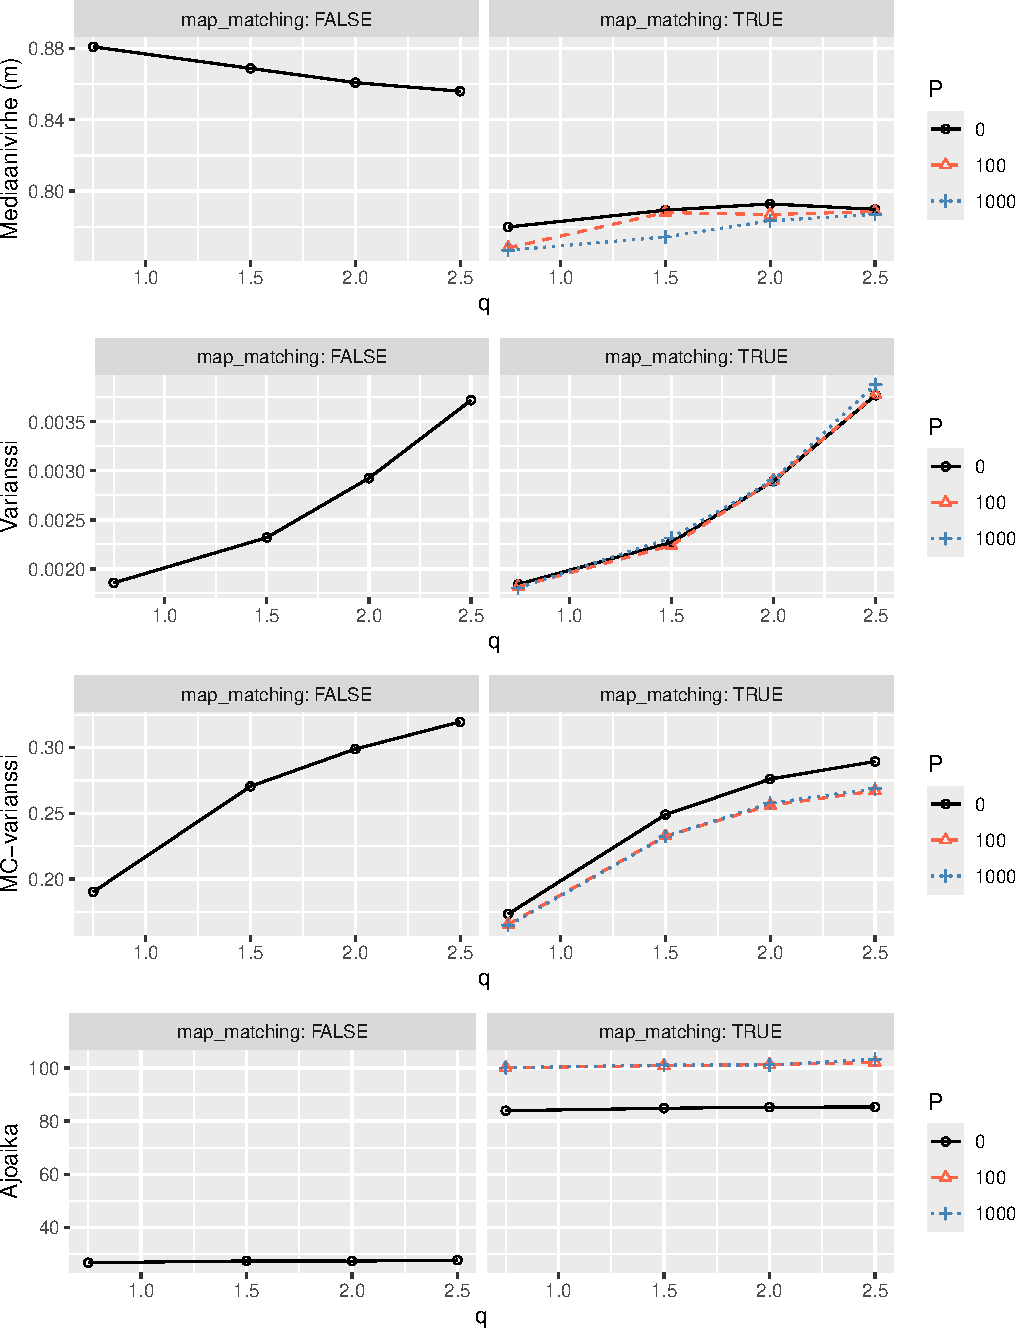
\includegraphics[width=15cm,height=20cm]{output/figures/phase2-results-1} 

}

\caption{Vaiheen 2 tulokset}\label{fig:phase2-results}
\end{figure}

Toisen vaiheen tuloksista huomataan, että karttasovituksen käyttäminen parantaa paikannusvirhettä. Syy tähän on helppo havaita liitteenä olevista karttapoluista. Paikannus ottaa nyt huomioon sisätilaympäristön, eikä enää luo estimaatteja sijainteihin, joihin tagin on fyysisesti mahdotonta päästä. Samoin rangaistusarvo \(P\):n lisääminen parantaa paikannusvirhettä. Tämä on odotettua, sillä isomman rangaistusarvon käyttäminen ei ainoastaan estä fyysisesti mahdottomia sijainteja vaan estää myös osan fyysisesti mahdottomista siirtymistä kahden peräkkäisen sijaintiestimaatin välillä.

Vastaavasti liikemallin kohina-arvon \(q\) pienentäminen parantaa paikannusvirhettä. Liian pienellä \(q\)-arvolla algoritmi ei kuitenkaan enää tutki signaaliympäristöä tarpeeksi tehokkaasti ja paikannusvirhe kasvaa. Samoin kasvaa estimaattien MC-varianssi. Paikannusvirheen mielessä paras kohina-arvo on tulosten perusteella \(q=0.75\). Tämä vastaa hyvin kirjallisuudessa esitettyjä keskimääräisiä kävelynopeuksia (kts. esim. \citep{Ho-2016}), kun huomioidaan, että kyse on kauppaympäristöstä. Vaikka parametri on tutkitun parametriavaruuden reunalla, ei tästä syystä alempia \(q\)-arvoja ole enää tarpeen tutkia, sillä alemmat arvot eivät enää vastaisi realistisia kävelynopeuksia.

Huomataan lisäksi, että parhaimman paikannusvirheen tuottava rangaistusarvo \(P=1000\) on tutkitun parametriavaruuden reunalla, joten mahdollisesti isommalla \(P\)-arvolla voitaisiin vielä parantaa paikannusvirhettä. Pienempien \(P\)-arvojen paikannusvirheiden luottamusvälit ovat kuitenkin päällekäisiä arvon \(P=1000\) kanssa, joten paikannusvirheeseen saatu lisähyöty ei todennäköisesti olisi tilastollisesti merkitsevää. Näiden tulosten perusteella valitaan viimeiseen vaiheeseen kiinteät arvot \emph{map\_matching}\(=T\), \(P=1000\) ja \(q=0.75\).

Viimeisessä vaiheessa testattiin datan valinnassa käytettävää signaalin vahvuuden kynnysarvoa \emph{rssi\_threshold} \(={-120, -100,-90,-80}\) sekä prediktiivistä siloitinta \emph{smoothing} \(={T,F}\) eli kahdeksaa eri suunnitteluparametrikombinaatiota. Tulokset on esitetty kuvassa \(\ref{fig:phase3-results}\) sekä taulukoissa \ref{tab:vaihe-3-tulokset} ja \ref{tab:vaihe-3-tulokset-varianssi}. Ajojen tulokset on esitetty karttapolkuina liitteen A alaluvussa \nameref{vaihe-3}.

\begin{table}

\caption{\label{tab:vaihe-3-tulokset}Vaiheen 3 tulokset, paikannusvirhe}
\centering
\begin{tabular}[t]{rlrlr}
\toprule
rssi\_threshold & smoothing & Mediaani (m) & Mediaanin 95\%-luottamusväli & <1m\\
\midrule
-120 & TRUE & 0.78 & {}[0.77, 0.79] & 0.60\\
-100 & TRUE & 0.78 & {}[0.77, 0.79] & 0.60\\
-90 & TRUE & 0.78 & {}[0.77, 0.78] & 0.61\\
-80 & TRUE & 0.81 & {}[0.8, 0.81] & 0.59\\
-120 & FALSE & 0.77 & {}[0.76, 0.77] & 0.63\\
\addlinespace
-100 & FALSE & 0.77 & {}[0.76, 0.77] & 0.63\\
-90 & FALSE & 0.76 & {}[0.76, 0.77] & 0.62\\
-80 & FALSE & 0.79 & {}[0.78, 0.79] & 0.59\\
\bottomrule
\end{tabular}
\end{table}

\begin{table}

\caption{\label{tab:vaihe-3-tulokset-varianssi}Vaiheen 3 tulokset, varianssi ja ajoaika}
\centering
\begin{tabular}[t]{rlrrr}
\toprule
rssi\_threshold & smoothing & Varianssi & MC-varianssi & Ajoaika (s)\\
\midrule
-120 & TRUE & 0 & 0.04 & 59.12\\
-100 & TRUE & 0 & 0.04 & 58.73\\
-90 & TRUE & 0 & 0.07 & 57.52\\
-80 & TRUE & 0 & 0.07 & 51.68\\
-120 & FALSE & 0 & 0.08 & 49.35\\
\addlinespace
-100 & FALSE & 0 & 0.08 & 49.32\\
-90 & FALSE & 0 & 0.08 & 48.90\\
-80 & FALSE & 0 & 0.12 & 46.35\\
\bottomrule
\end{tabular}
\end{table}

\clearpage

\begin{figure}

{\centering 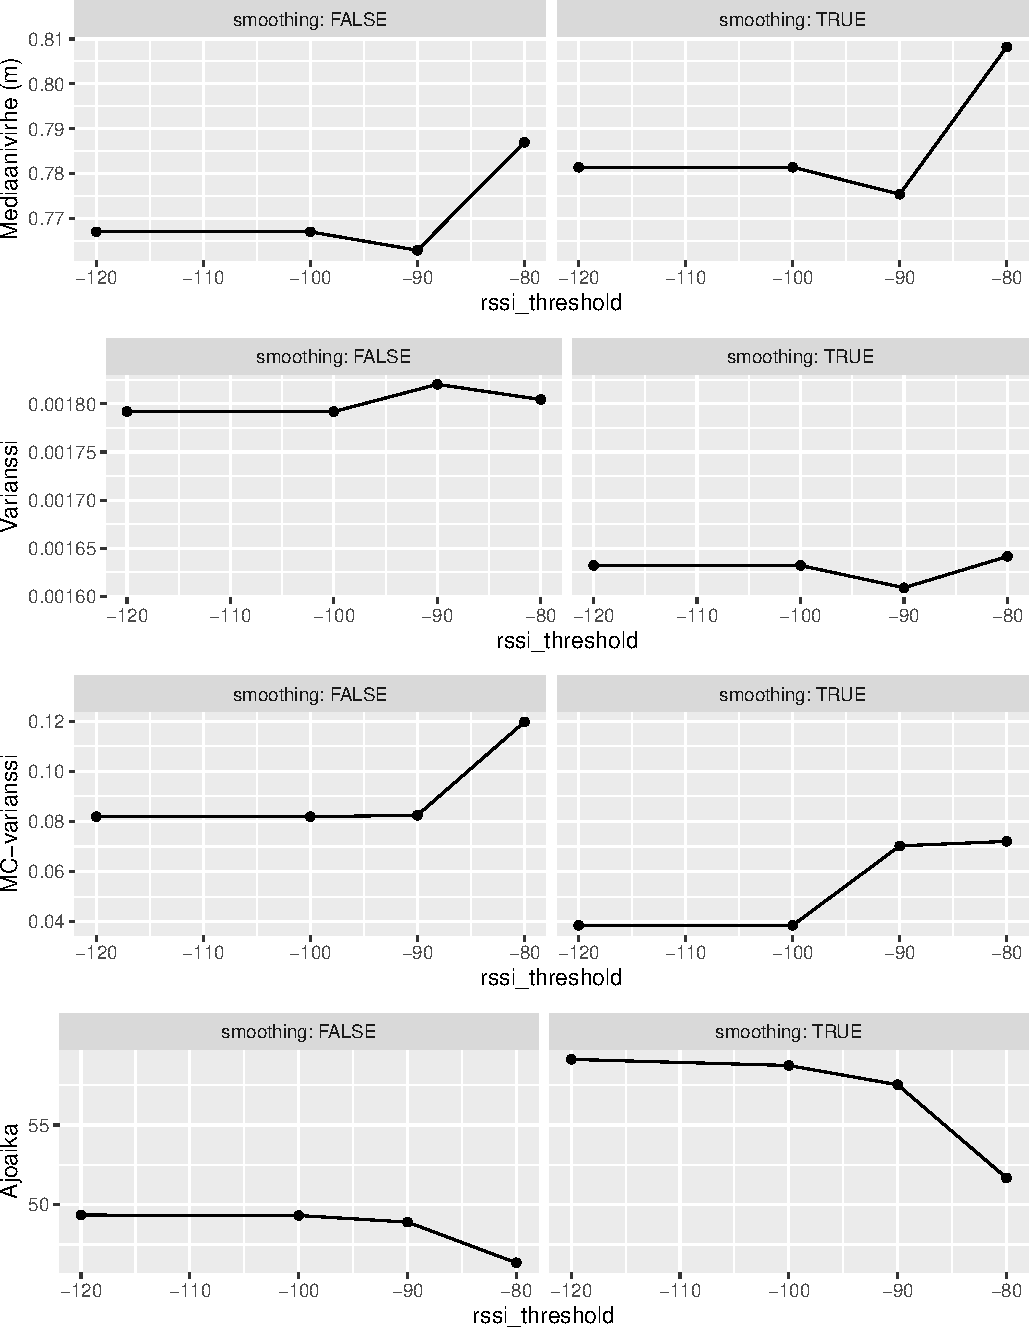
\includegraphics[width=15cm,height=20cm]{output/figures/phase3-results-1} 

}

\caption{Vaiheen 3 tulokset}\label{fig:phase3-results}
\end{figure}

Tuloksista huomataan, ettei siloittelun käyttäminen paranna paikannusvirhettä. Tämä on odotettua, koska liikemallina on käytetty satunnaiskulkua. Liitteenä olevista karttapoluista kuitenkin huomataan, että siloittelu tuottaa odotetusti sileämpiä polkuja, mikä saattaa olla käytännössä haluttu ominaisuus. Sen sijaan signaalin vahvuuden kynnysarvon nostaminen arvoon \emph{rssi\_threshold} \(=-90\) parantaa hieman paikannustarkkuutta. Kynnysarvon käyttö myös nopeuttaa algoritmin ajoaikaa, sillä kynnysarvoa käytettäessä uskottavuusfunktio (\ref{lopullinen-uskottavuusmalli}) lasketaan pienemmästä määrästä otoksia. Valitaan näin kolmannen vaiheen tulosten perusteella parametrit \emph{smoothing=F} ja \emph{rssi\_threshold}=\(-90\).

Taulukossa \ref{tab:tulokset-final} on esitetty yhteenvetona kaikkien koevaiheiden tulosten perusteella valitut suunnitteluparametrit. Täydet eri koevaiheiden tulokset löytyvät csv-muodossa osoitteista \newline \url{https://github.com/rintakumpu/progradu/blob/main/analyysi/data/tulokset_vaihe1_ci.csv} (vaihe 1) \newline \url{https://github.com/rintakumpu/progradu/blob/main/analyysi/data/tulokset_vaihe2_ci.csv} (vaihe 2) ja \newline \url{https://github.com/rintakumpu/progradu/blob/main/analyysi/data/tulokset_vaihe3_ci.csv} (vaihe 3). Kansio \url{https://github.com/rintakumpu/progradu/blob/main/analyysi/data/} sisältää lisäksi RDS-muotoon tallennettuna kaikkien ajojen tulokset.

\begin{table}

\caption{\label{tab:tulokset-final}Tulosten perusteella valitut suunnitteluparametrit}
\centering
\begin{tabular}[t]{ll}
\toprule
Suunnitteluparametri & Arvo\\
\midrule
N & 1000\\
resampling & 0.67\\
map\_matching & TRUE\\
P & 1000\\
q & 0.75\\
\addlinespace
smoothing & FALSE\\
rssi\_threshold & -90\\
\bottomrule
\end{tabular}
\end{table}

Tulosten perusteella voidaan todeta, että WB-sisätilapaikannusalgoritmi tuottaa halutun paikannusvirheen. Algoritmin testaamisessa on myös käytetty todelliseen liiketilaan luotua testiasetelemaa, joka vastaa hyvin järjestelmän todellista käyttötarkoitusta. Tämän perusteella voidaan algoritmin myös olettaa yleistyvän hyvin monimutkaisiin sisätilaympäristöihin. Taulukossa \ref{tab:tulokset-total} on esitetty ToTal-triangulaatioalgoritmilla \ref{total} luoduista sijaintiestimaateista laskettujen paikannusvirheiden tunnuslukuja.

\begin{table}

\caption{\label{tab:tulokset-total}ToTal-triangulaatioalgoritmin tuottamia paikannusvirheen tunnuslukuja}
\centering
\begin{tabular}[t]{lrrrr}
\toprule
  & Mediaani & Aritmeettinen keskiarvo & Otoskeskihajonta & <1m persentiili\\
\midrule
ToTaL & 1.61 & 2.35 & 4.15 & 0.34\\
\bottomrule
\end{tabular}
\end{table}

Triangulaatioon verrattuna WB-sisätilapaikannusalgoritmi tuottaa huomattavasti parempia tuloksia. Tämän voi havaita myös vertaamalla kuvan \ref{fig:total-karttapolku} ToTal-karttapolkua liitteen A WB-sisätillapaikannusalgoritmin tuottamiin karttapolkuihin.

\begin{figure}[H]
\centering
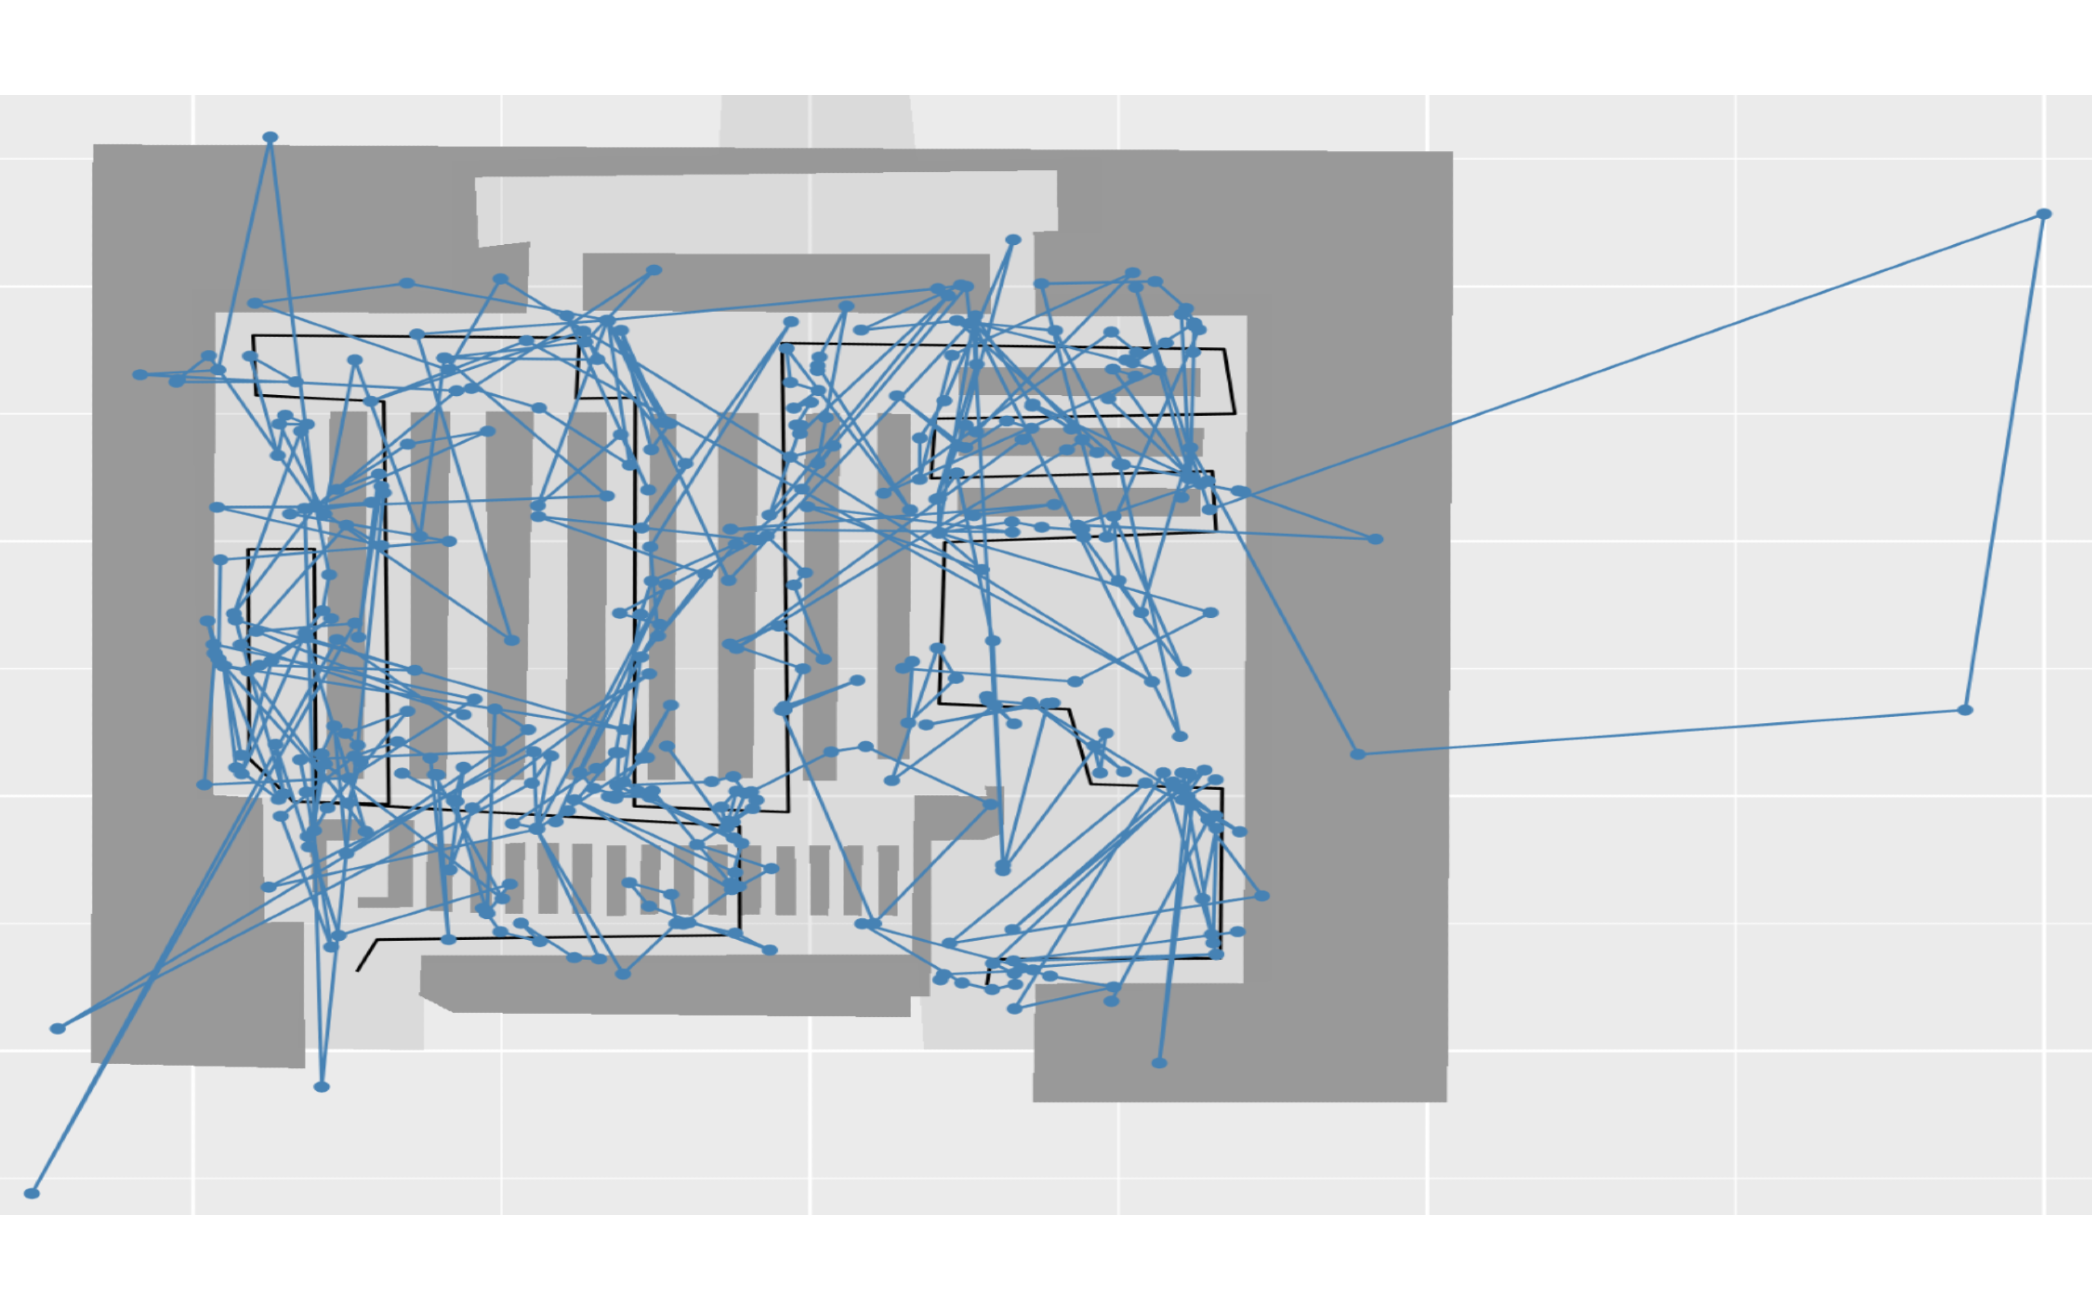
\includegraphics[width=15cm]{total-karttapolku}
\caption{ToTal-triangulaatioalgoritmin tuottamat sijaintiestimaatit}
\label{fig:total-karttapolku}
\end{figure}

Algoritmia ja järjestelmää voitaisiin mahdollisesti edelleen parantaa esimerkiksi käyttämällä tagia, jonka kiihtyvyysmittarin tuottama data olisi käytettyä tagia luotettavampaa. Dataa voitaisiin hyödyntää esimerkiksi informatiivisen liikemallin luomisessa. Tällöin olisi myös mielekkäämpää toteuttaa varianssiestimaattiin perustuva adaptiivisen viipeen suodin osana paikannusalgoritmia. Lisäksi datan valinta voitaisiin suorittaa esimerkiksi niin, että datasta poistettaisiin kullakin aika-askeleella ne kulmahavainnot, jotka poikkeavat kulmahavaintojen suuntakonsensuksesta.

Liitteenä olevia polkuja tarkastelemalla huomataan, että nyt toteutetun algoritmin sijantiestimaatilla on taipumus jäädä osassa testiympäristöä jälkeen itse tagin sijainnista. Tätä ongelmaa voitaisiin mahdollisesti lieventää käyttämällä mm. Yi Chenging \&al.~artikkelissa ``Improved Particle Filter Algorithm for Multi-Target Detection and Tracking'' (2024) \citep{Cheng-2024} esittämää menetelmää, jossa partikkelit jaetaan ns. seurantahiukkasiin sekä etsintähiukkasiin, joista ainoastaan edellisiä käytetään sijaintiestimaatin luomisessa ja jälkimmäisten annetaan liikkua suuremmilla kohina-arvoilla. Näin mahdollistetaan satunnaiskulkumallilla laajempi signaaliavaruuden tutkinta ja nopeampi ongelmatilanteista toipuminen ilman, että sijaintiestimaatit kärsivät liikemalliin lisätystä kohinasta.

\hypertarget{lopuksi}{%
\chapter{Lopuksi}\label{lopuksi}}

Tässä tutkielmassa on esitetty pääpiirteittäin hiukkassuodin- ja hiukkassiloitinalgoritmien teoria Bayesilaisessa tilastotieteellisessä viitekehyksessä. Tutkielmassa on lisäksi käyty läpi uudelleenotantaa efektiivisen otoskoon perusteella hyödyntävä SIR-suodinalgoritmi sekä käsitelty algoritmin varianssin estimointia. Tutkielmassa on myös esitetty SIR-algoritmin parametrien valintaan, suorituskykyyn sekä konvergenssiin liittyviä tuloksia.

Tutkielmassa on lisäksi esitetty WB-sisätilapaikannusalgoritmi, joka toteuttaa SIR-algoritmin, varianssin estimoinnin sekä hyödyntää sisätilapaikannuksen karttasovitusalgoritmia. Tutkielmassa on lopuksi tarkasteltu miten eri suunnitteluparametrien valinnat vaikuttavat algoritmin suorituskykyyn kattavan, todelliseen ongelmaan ja dataan perustuvan paikannusesimerkin avulla.

\hypertarget{liite-a---karttapolut}{%
\chapter*{Liite A - Karttapolut}\label{liite-a---karttapolut}}
\addcontentsline{toc}{chapter}{Liite A - Karttapolut}

Liite sisältää tutkielman tulososioon liittyvät karttapolut. Kukin kartta käsittää \(r=30\) ajoa kullakin suunnitteluparametrikombinaatiolla. Karttojen otsikossa on mainittu ainoastaan testatut suunnitteluparametrit, vakioarvoiset parametrit on esitetty luvussa \ref{tulokset}.

\hypertarget{vaihe-1}{%
\section*{Vaihe 1}\label{vaihe-1}}
\addcontentsline{toc}{section}{Vaihe 1}

\begin{center}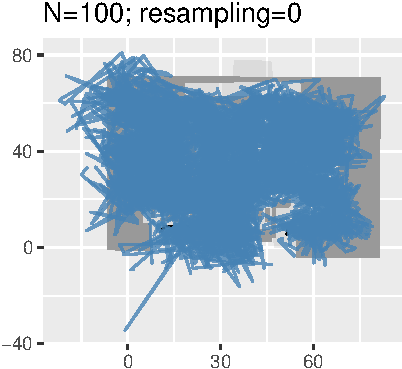
\includegraphics{output/figures/unnamed-chunk-1-1} 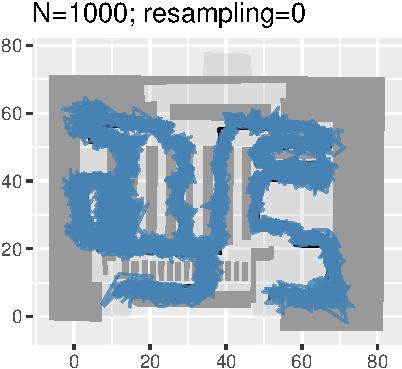
\includegraphics{output/figures/unnamed-chunk-1-2} 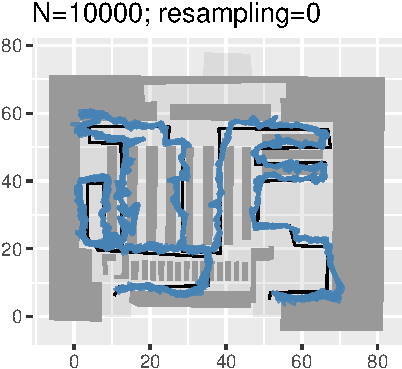
\includegraphics{output/figures/unnamed-chunk-1-3} 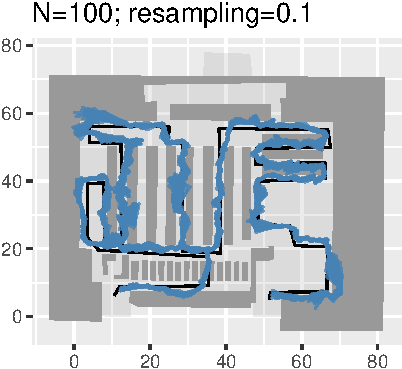
\includegraphics{output/figures/unnamed-chunk-1-4} 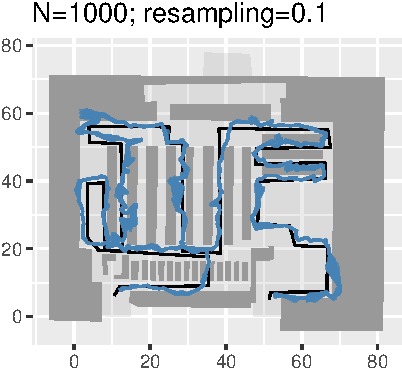
\includegraphics{output/figures/unnamed-chunk-1-5} 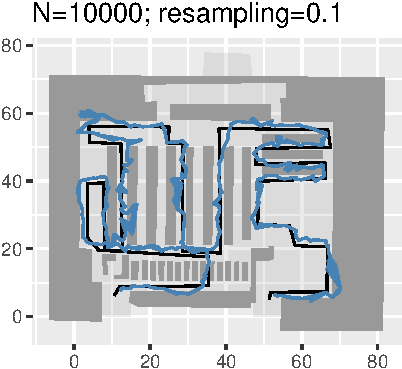
\includegraphics{output/figures/unnamed-chunk-1-6} 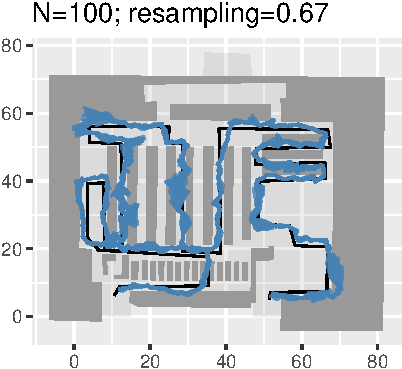
\includegraphics{output/figures/unnamed-chunk-1-7} 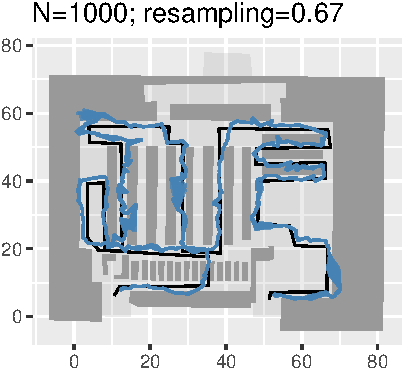
\includegraphics{output/figures/unnamed-chunk-1-8} 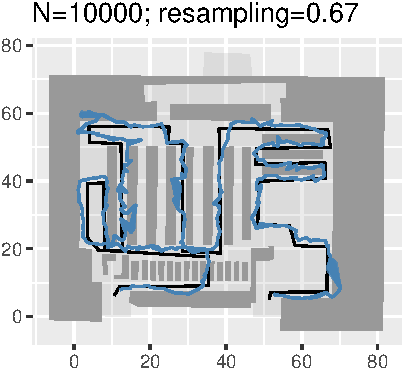
\includegraphics{output/figures/unnamed-chunk-1-9} 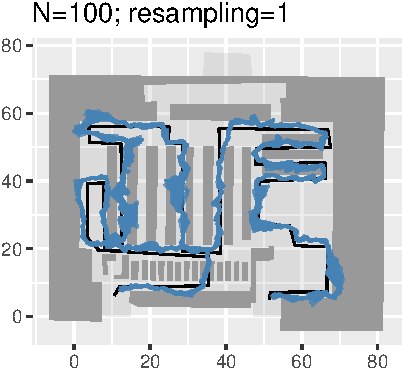
\includegraphics{output/figures/unnamed-chunk-1-10} 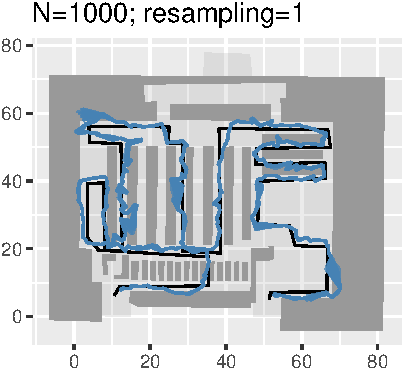
\includegraphics{output/figures/unnamed-chunk-1-11} 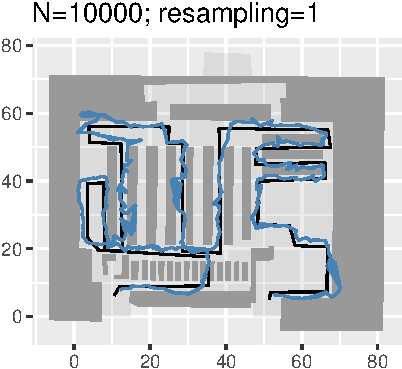
\includegraphics{output/figures/unnamed-chunk-1-12} \end{center}

\hypertarget{vaihe-2}{%
\section*{Vaihe 2}\label{vaihe-2}}
\addcontentsline{toc}{section}{Vaihe 2}

\begin{center}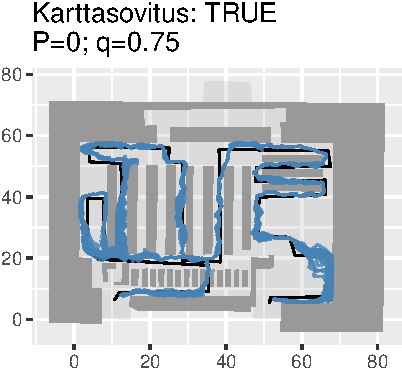
\includegraphics{output/figures/unnamed-chunk-2-1} 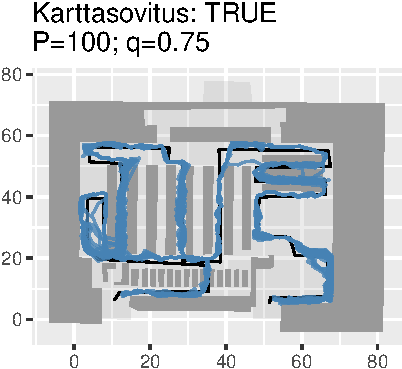
\includegraphics{output/figures/unnamed-chunk-2-2} 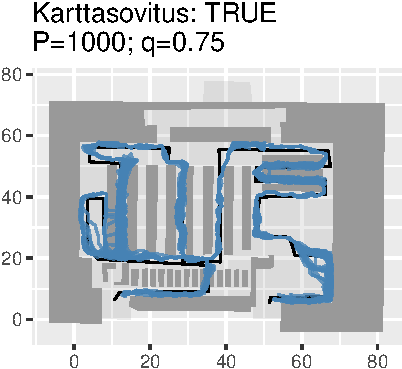
\includegraphics{output/figures/unnamed-chunk-2-3} 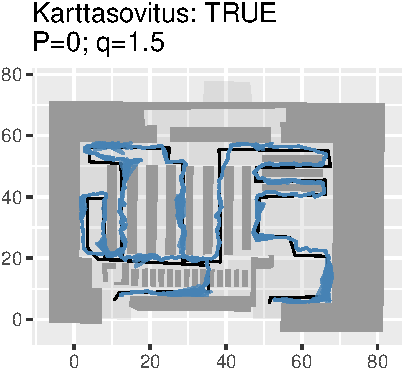
\includegraphics{output/figures/unnamed-chunk-2-4} 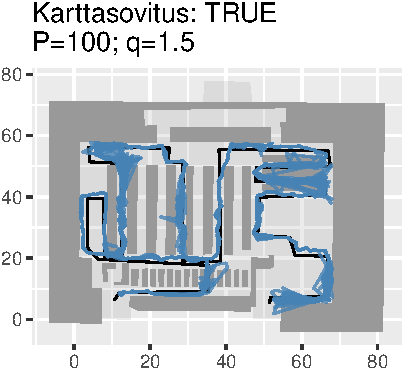
\includegraphics{output/figures/unnamed-chunk-2-5} 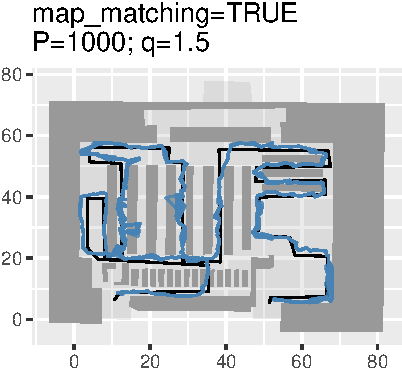
\includegraphics{output/figures/unnamed-chunk-2-6} 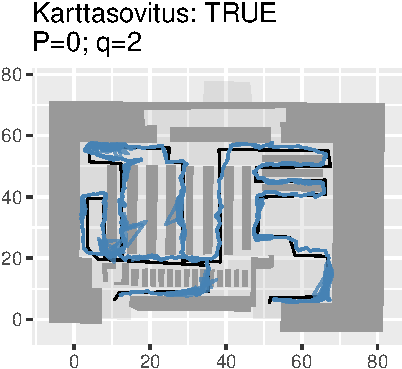
\includegraphics{output/figures/unnamed-chunk-2-7} 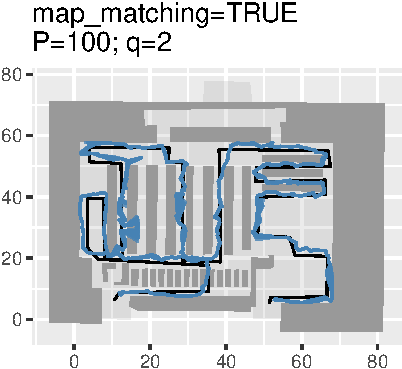
\includegraphics{output/figures/unnamed-chunk-2-8} 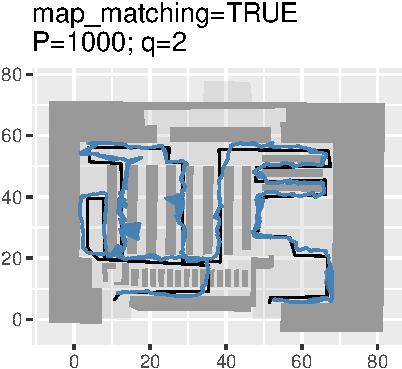
\includegraphics{output/figures/unnamed-chunk-2-9} 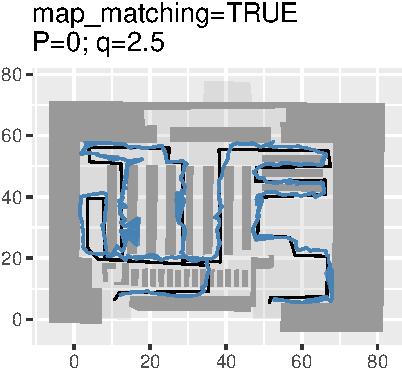
\includegraphics{output/figures/unnamed-chunk-2-10} 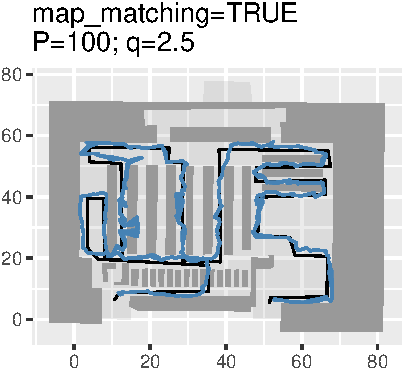
\includegraphics{output/figures/unnamed-chunk-2-11} 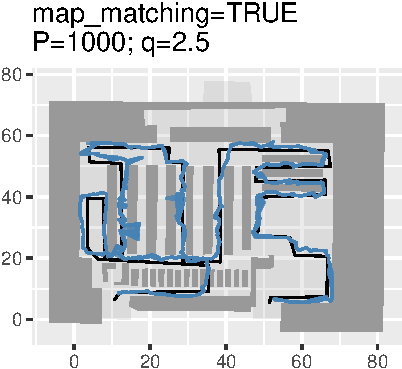
\includegraphics{output/figures/unnamed-chunk-2-12} 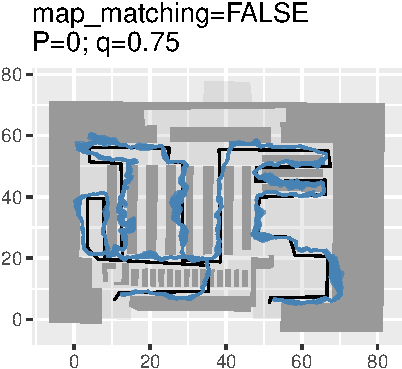
\includegraphics{output/figures/unnamed-chunk-2-13} 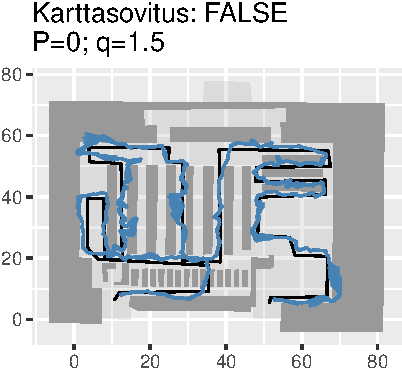
\includegraphics{output/figures/unnamed-chunk-2-14} 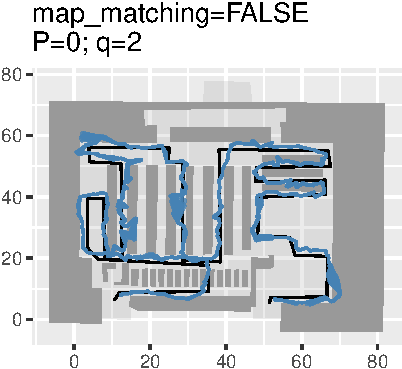
\includegraphics{output/figures/unnamed-chunk-2-15} 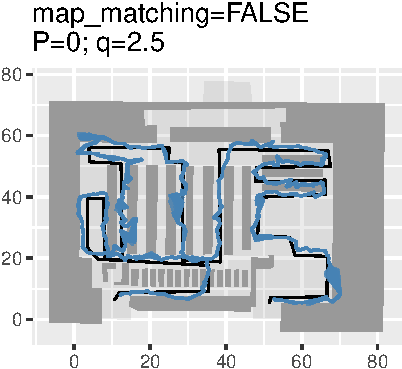
\includegraphics{output/figures/unnamed-chunk-2-16} \end{center}

\hypertarget{vaihe-3}{%
\section*{Vaihe 3}\label{vaihe-3}}
\addcontentsline{toc}{section}{Vaihe 3}

\begin{center}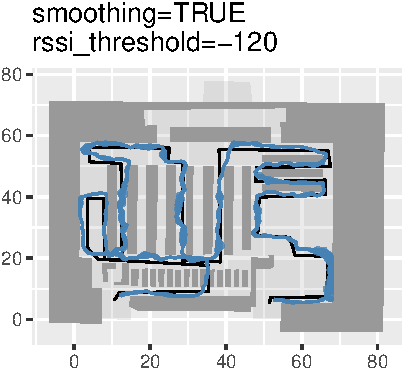
\includegraphics{output/figures/unnamed-chunk-3-1} 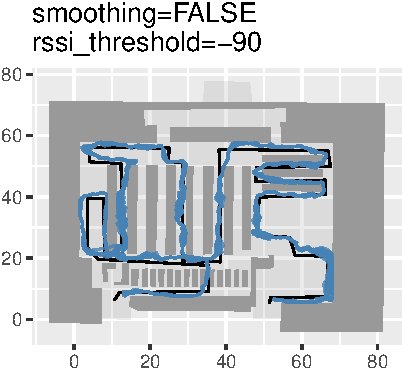
\includegraphics{output/figures/unnamed-chunk-3-2} 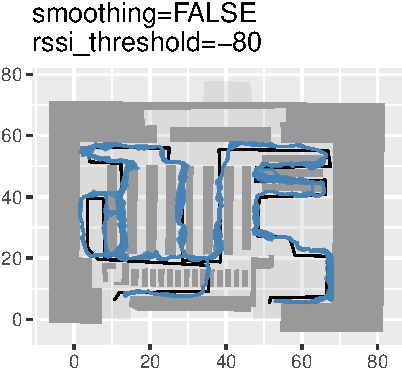
\includegraphics{output/figures/unnamed-chunk-3-3} 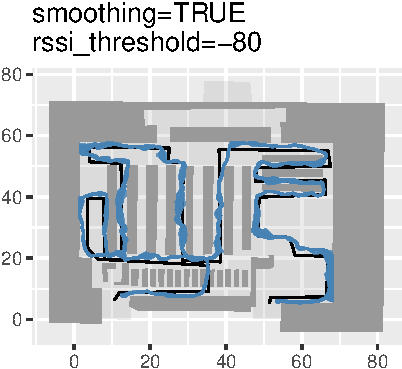
\includegraphics{output/figures/unnamed-chunk-3-4} 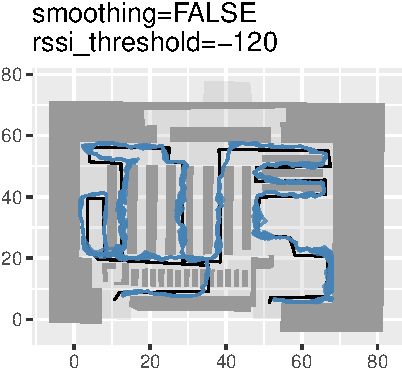
\includegraphics{output/figures/unnamed-chunk-3-5} 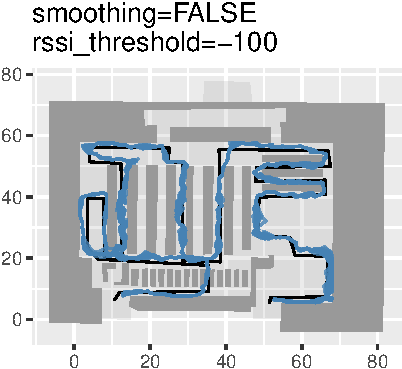
\includegraphics{output/figures/unnamed-chunk-3-6} \includegraphics{output/figures/unnamed-chunk-3-7} \includegraphics{output/figures/unnamed-chunk-3-8} \end{center}

  \bibliography{packages.bib,lahteet.bib}

\end{document}
